\documentclass{article}
\usepackage{geometry}
\geometry{
	a4paper,
	left=2.5cm,
	right=2.5cm,
	top=2.5cm,
	bottom=2.5cm,
	headheight=13.6pt
}

% 最简单、最稳定的中文方案（自动适配系统，永不报错）
\usepackage[UTF8, scheme=plain]{ctex}

% 设置英文默认字体为 Times New Roman
\usepackage{fontspec}
\setmainfont{Times New Roman}

\usepackage{amsmath}
\usepackage{amssymb}
\usepackage{booktabs}
\usepackage{caption}
\usepackage{setspace}
\doublespacing
\setlength{\parskip}{4pt}

\usepackage{array}
\usepackage{listings}
\usepackage{graphicx}
\usepackage{enumitem}
\usepackage{subcaption}
\usepackage{multirow}
\usepackage{mathrsfs}
\usepackage{bm}
\usepackage{xcolor}
\usepackage{colortbl}

\usepackage{tikz}
\usepackage{tikz-3dplot}
\usetikzlibrary{
	arrows.meta,
	calc,
	patterns,
	decorations.pathmorphing,
	backgrounds,
	positioning,
	fit,
	shapes.geometric,
	intersections,
	through,
	angles,
	quotes,
	plotmarks
}

%目录超链接
\usepackage{hyperref}
\hypersetup{
	colorlinks=true,
	linkcolor=black,
	filecolor=magenta,
	urlcolor=cyan,
}
\usepackage{tocloft}
\setlength{\cftbeforesecskip}{2ex}
\setlength{\cftbeforesubsecskip}{1ex}
\setlength{\cftbeforesubsubsecskip}{1ex}

% 定义代码颜色
\definecolor{codegreen}{rgb}{0,0.6,0}
\definecolor{NavyBlue}{RGB}{0,0,128}
\definecolor{PineGreen}{RGB}{1,121,111}

% 配置 listings 环境
\lstset{
	language=TeX,
	tabsize=4,
	captionpos=b,
	numbers=left,
	numbersep=1em,
	sensitive=true,
	showtabs=false,
	frame=shadowbox,
	breaklines=true,
	keepspaces=true,
	showspaces=false,
	showstringspaces=false,
	breakatwhitespace=false,
	basicstyle=\ttfamily\normalsize,
	keywordstyle=\color{NavyBlue},
	commentstyle=\color{codegreen},
	numberstyle=\color{black},
	stringstyle=\color{PineGreen!90!black},
	rulesepcolor=\color{red!20!green!20!blue!20},
	escapeinside={/@}{@/},
}

% 自定义颜色
\definecolor{LightGreen}{rgb}{0.9, 0.95, 0.9}
\definecolor{LightBlue}{RGB}{229, 238, 255}
\definecolor{LightPink}{RGB}{255, 229, 237}
\definecolor{DarkRed}{RGB}{169,0,0}
\definecolor{DarkGreen}{RGB}{0,110,12}
\definecolor{SkyBlue}{RGB}{0,114,255}

% 自定义环境 无缩进
\newenvironment{knowledge}[1]{%
	\noindent{\normalfont\bfseries\color{DarkRed} #1}\hskip 0.5em%
	\color{DarkRed}%
}{%
	\par\color{black}%
}

\newenvironment{question}[1][]{%
	\noindent
	\ifx\relax#1\relax\else
	{\normalfont\color{DarkGreen} #1}\hskip 0.5em%
	\fi
	\color{DarkGreen}%
}{%
	\ifhmode\fi\color{black}%
}

\newcommand{\category}[1]{\noindent{\normalfont\bfseries\color{SkyBlue} #1}\hskip 0.5em}

\captionsetup[table]{
	justification=centering,
	labelsep=quad,
	font={bf}
}
\captionsetup[figure]{
	justification=centering,
	labelsep=quad,
	font={bf}
}
\captionsetup[subfigure]{
	font={bf}
}

\begin{document}

\begin{center}
	{\LARGE \textbf{高中数学笔记}} \\[0.5cm]
	{\large {\kaishu 石继楷 \quad 编写}} \\[0.3cm]
	{\normalsize 2026年7月28日}
\end{center}

\tableofcontents
\newpage


\section{初升高暑期数学}

\subsection{第一讲\quad 二次方程拓展}

\subsubsection{因式分解}
\begin{knowledge}{因式分解}
	
	公式：$a^3-b^3=(a-b)(a^2+ab+b^2)$
	
	$a^3+b^3=(a+b)(a^2-ab+b^2)$.
	
	提公因式$\to$公式$\to$十字相乘$\to$分组分解.
	
	$x,y,z$未知数 / $a,b,c$为参数.
\end{knowledge}
	
\begin{question}
	
	eg1：$m+5n-mn-5n^2=m-mn+5n-5n^2=(1-n)(m+5n)$.
	
	eg2：$-7x^2+19x+6=(7x+2)(-x+3)$.
	
	eg3：$x^2-(3m+2)x+3m+1=(x-3m-1)(x-1)$.
	
\end{question}

\subsubsection{解含参方程}
\begin{knowledge}{一次含参}
	
	\begin{question}
	eg1：$mx=2$，一次含参需分类讨论.
	\end{question}
	
	\begin{enumerate}[label=\arabic*., left=0pt]
		
		\item 当$m=0$时，$0x=2$无解$\Rightarrow\varnothing$（空集）.
		
		\item 当$m\neq0$时，$x=\dfrac{2}{m}$.
		
	\end{enumerate}
	
	总结：提$x$；讨论$x$系数是否为$0$.
	
	\begin{question}
	eg2：$mx-3=-x \implies (m+1)x=3$.
	\end{question}
	
	\begin{enumerate}[label=\arabic*., left=0pt]
		
		\item 当$m+1=0$，即$m=-1$时：$0\cdot x=3$，$\varnothing$.
		
		\item 当$m+1\neq0$，即$m\neq-1$时：$x=\dfrac{3}{m+1}$.
		
	\end{enumerate}
\end{knowledge}

\begin{knowledge}{二次含参}
	
	总结：
	
	因式分解（eg1）
	
	求根公式（eg2）
	
	因式分解讨论两解是否相同
	
	求根公式讨论$\Delta$与0的关系
	
	\begin{question}
	eg1：$(x-1)(x-a)=0$.
	\end{question}
	
	\begin{enumerate}[label=\arabic*., left=0pt]
		
		\item 当$a=1$时，$x_1=x_2=1$.
		
		\item 当$a\neq1$时，$x_1=1$，$x_2=a$.
		
	\end{enumerate}

\begin{question}
	eg2：$x^2+x+a=0$，$\Delta=1-4a$.
\end{question}
	
	\begin{enumerate}[label=\arabic*., left=0pt]
		
		\item 当$\Delta=1-4a>0$，即$a<\dfrac{1}{4}$时：$x_1=\dfrac{-1-\sqrt{1-4a}}{2}$，$x_2=\dfrac{-1+\sqrt{1-4a}}{2}$.
		
		\item 当$\Delta=1-4a=0$，即$a=\dfrac{1}{4}$时：$x_1=x_2=-\dfrac{1}{2}$.
		
		\item 当$\Delta=1-4a<0$，即$a>\dfrac{1}{4}$时：$\varnothing$.
		
	\end{enumerate}
	
	综上：当$a<\dfrac14$时两根；当$a=\dfrac14$时一根；当$a>\dfrac14$时无根.
\end{knowledge}

\subsubsection{韦达定理}
\begin{knowledge}{韦达定理}
	
	推：$|x_1-x_2|=\dfrac{\sqrt{\Delta}}{|a|}$.
	
	四大金刚：$a+b$，$ab$，$(a-b)$，$a^2+b^2$，知二求二.
	
	$(a-b)=\sqrt{(a-b)^2}=\sqrt{a^2+b^2-2ab}=\sqrt{(a+b)^2-4ab}$.
	
	$|x_1-x_2|=\sqrt{(x_1+x_2)^2-4x_1x_2}=\sqrt{\left(-\dfrac{b}{a}\right)^2-4\cdot\dfrac{c}{a}}=\sqrt{\dfrac{b^2-4ac}{a^2}}=\dfrac{\sqrt{\Delta}}{|a|}$.
	
	注意：当所求式无法用韦达定理时，把二次项根带回原方程中进行降次.
\end{knowledge}

\category{降次}
\begin{question}
	原方程$x^2-x-1=0$，求$x_1^2+x_2$.
\end{question}

分析：把$x_1$带回原方程中得$x_1^2-x_1-1=0 \implies x_1^2=x_1+1$.

$x_1^2+x_2=x_1+x_2+1=1+1=2$.

\subsection{第二讲\quad 解不等式}

\subsubsection{不等式的性质}
\begin{knowledge}{不等式的性质}
	
	$a>b,\ b>c \implies a>c$.
	
	$a>b \implies a+c>b+c$.
	
	$a>b,\ c>d \implies a+c>b+d$（同向可加）.
	
	$a>b>0,\ c>d>0 \implies ac>bd$（同向可乘）.
	
	证明不等式的方法：作差比较法：$a>b \iff a-b>0$.
\end{knowledge}

\category{求范围}
\begin{question}
	$1<a<2$，$2<b<4$，求$a+2b$的范围；求$b-a$的范围.
\end{question}

$4<2b<8$.

$\therefore 5<a+2b<10$.

$b-a=b+(-a)$；$-2<-a<-1$.

$\therefore 0<b-a<3$.

\category{判断符号}
\begin{question}
	(1)$a>b$，则$a^2>b^2$？(2)$a>b>0$，$c<d<0$，比较$\dfrac{a}{d}$与$\dfrac{b}{c}$，$\dfrac{a}{c}$与$\dfrac{b}{d}$.
\end{question}

(1) 正误：$a^2-b^2=(a+b)(a-b)$，$(a+b)$符号？，$(a-b)>0$.

(2) 关键理解：$ac<bd$.

可判断$\dfrac{a}{d}<\dfrac{b}{c}$；不可判断$\dfrac{a}{c}$与$\dfrac{b}{d}$.

\subsubsection{解一元二次不等式}
\begin{knowledge}{步骤}
	\begin{enumerate}[label=\arabic*., left=0pt]
		
		\item 化标准：二次项系数化为正.
		
		\item 求根.
		
		\item 大于取两边，小于夹中间.
		
	\end{enumerate}
\end{knowledge}

\category{解不等式}
\begin{question}
	$-2x^2+x+3\leq0$.
\end{question}

\begin{enumerate}[label=\arabic*., left=0pt]
	
	\item $2x^2-x-3\geq0$.
	
	\item $2x^2-x-3=0$：$x_1=-1$，$x_2=\dfrac{3}{2}$.
	
	\item $x\leq-1$或$x\geq\dfrac{3}{2}$.
	
\end{enumerate}

\category{由解求ab}
\begin{question}
	$ax^2+bx-2>0$的解是$x<-\dfrac{1}{2}$或$x>\dfrac{1}{3}$，则$ab=$？
\end{question}

两根为$-\dfrac{1}{2},\dfrac{1}{3}$：根之积$=-\dfrac{2}{a}=-\dfrac{1}{6} \implies a=12$.

根之和$=-\dfrac{b}{a}=-\dfrac{1}{6} \implies b=2$.

$\therefore ab=24$.

\category{Delta=0}
\begin{question}
	$x^2-4x+4>0$.
\end{question}

\begin{minipage}[t]{0.7\textwidth}
	$\Delta=0$.
	
	$\therefore x\in\{x|x\neq2\}$.
	
	（若$\Delta\leq0$，则画图像确定.）
\end{minipage}
\hfill
\begin{minipage}[t]{0.3\textwidth}
	\centering
	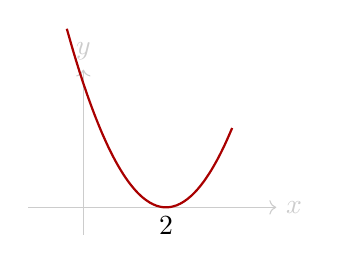
\begin{tikzpicture}[scale=0.7, baseline=(current bounding box.north)]
		\draw[->, gray!40] (-1,0) -- (3.5,0) node[right] {$x$};
		\draw[->, gray!40] (0,-0.5) -- (0,2.5) node[above] {$y$};
		\draw[thick, DarkRed, domain=-0.3:2.7, smooth, variable=\x] plot ({\x}, {(\x-1.5)*(\x-1.5)});
		\node[below] at (1.5,0) {$2$};
	\end{tikzpicture}
\end{minipage}

\subsubsection{解分式不等式}
\begin{knowledge}{步骤}
	\begin{enumerate}[label=\arabic*., left=0pt]
		
		\item 移项通分.
		
		\item 化除为乘.
		
		\item 按一元二次不等式的方法解不等式.
		
	\end{enumerate}
	
	注意：当出现$\leq,\geq$时，分母不为$0$.
\end{knowledge}

\category{解分式不等式}
\begin{question}
	$\dfrac{-3x+4}{x-1}\geq2$.
\end{question}

$\dfrac{-5x+6}{x-1}\geq0 \implies \begin{cases} (5x-6)(x-1)\leq0 \\ x\neq1 \end{cases}$

$x_1=\dfrac{6}{5}$，$x_2=1$.

$\therefore 1<x\leq\dfrac{6}{5}$.

\subsection{第三讲\quad 解含参不等式}

\subsubsection{解绝对值不等式}
\begin{knowledge}{绝对值不等式}
	
	$|u|<a \implies -a<u<a$.
	
	$|u|>a \implies u<-a$或$u>a$.
	
	$|u|<|v| \implies u^2<v^2$.
\end{knowledge}

\category{绝对值不等式}
\begin{question}
	$|5-2x|>3$.
\end{question}

$5-2x<-3$或$5-2x>3$.

$\therefore x>4$或$x<1$.

\category{两边绝对值}
\begin{question}
	$|x-1|<|x-3|$.
\end{question}

$(x-1)^2<(x-3)^2$.

$\therefore x<2$.

\category{两边绝对值}
\begin{question}
	$|x+1|<|2x+1|$.
\end{question}

$(x+1)^2<(2x+1)^2 \implies 3x^2+2x>0$.

$\therefore x>0$或$x<-\dfrac{2}{3}$.

\subsubsection{解一元一次含参不等式}
\begin{knowledge}{步骤}
	移项，提$x$.
	
	讨论系数正负零情况.
\end{knowledge}

\category{一次含参}
\begin{question}
	$mx>2$.
\end{question}

\begin{enumerate}[label=\arabic*., left=0pt]
	
	\item 当$m=0$时：$0\cdot x>2$，$\varnothing$.
	
	\item 当$m>0$时：$x>\dfrac{2}{m}$.
	
	\item 当$m<0$时：$x<\dfrac{2}{m}$.
	
\end{enumerate}

\subsubsection{解一元二次含参不等式}
\begin{knowledge}{步骤}
	化标准（讨论二次）.
	
	因式分解$\to$讨论根大小等；求根公式$\to$讨论$\Delta$正负零.
\end{knowledge}

\category{二次含参}
\begin{question}
	$(x+t)(x-1)<0$.
\end{question}

根$x_1=-t$，$x_2=1$.

\begin{enumerate}[label=\arabic*., left=0pt]
	
	\item 当$-t=1$即$t=-1$时：无解.
	
	\item 当$-t>1$即$t<-1$时：$1<x<-t$.
	
	\item 当$-t<1$即$t>-1$时：$-t<x<1$.
	
\end{enumerate}

\subsection{第四讲\quad 基本不等式}
\begin{knowledge}{基本不等式}
	$\dfrac{a+b}{2}\geq\sqrt{ab}$，即$a+b\geq2\sqrt{ab}$.
	
	\begin{enumerate}[label=\arabic*., left=0pt]
		
		\item 正.
		
		\item 定（$a+b$、$ab$构造定值）.
		
		\item 相等（$a$和$b$有机会相等）.
		
	\end{enumerate}
	
	1$^\circ$积定和最小；2$^\circ$和定积最大；3$^\circ$和与倒数和，使用"乘1法".
\end{knowledge}

\category{凑基本不等式}
\begin{question}
	$y=x^2+1+\dfrac{25}{x^2+1}$，求最小值.
\end{question}

$y\geq2\sqrt{25}=10$.

当$x^2+1=5$即$x=\pm2$时取等.

$\therefore y_{\min}=10$.

\category{拆项}
\begin{question}
	已知$x>0$，$y=\dfrac{x^2+2x+16}{x}$，求最小值.
\end{question}

$y=x+2+\dfrac{16}{x}\geq2\sqrt{16}+2=10$.

当$x=4$时取等.

$\therefore y_{\min}=10$.

\category{加减凑配}
\begin{question}
	$y=x^2+\dfrac{1}{x^2-1}$（$x^2>1$），求最小值.
\end{question}

$y=x^2-1+\dfrac{1}{x^2-1}+1\geq2+1=3$.

$(x^2-1)^2=1 \implies x^2-1=1 \implies x=\pm\sqrt{2}$.

$\therefore y_{\min}=3$.

\category{和定积最大}
\begin{question}
	$x,y>0$，$\dfrac{x}{5}+\dfrac{y}{6}=1$，求$xy$最大值.
\end{question}

$\dfrac{x}{5}+\dfrac{y}{6}\geq2\sqrt{\dfrac{xy}{30}}$.

$\therefore xy\leq\dfrac{15}{2}$.

$\begin{cases} \dfrac{x}{5}=\dfrac{y}{6} \\ \dfrac{x}{5}+\dfrac{y}{6}=1 \end{cases} \implies \begin{cases} x=\dfrac{5}{2} \\ y=3 \end{cases}$.

$\therefore xy_{\max}=\dfrac{15}{2}$.

\category{乘1法}
\begin{question}
	$m+n-2=0$（$mn>0$），$\left(\dfrac{1}{m}+\dfrac{2}{n}\right)_{\min}=$？
\end{question}

$m+n=2$.

$\left(\dfrac{1}{m}+\dfrac{2}{n}\right)=\left(\dfrac{1}{m}+\dfrac{2}{n}\right)(m+n)\cdot\dfrac{1}{2}=\left(3+\dfrac{n}{m}+\dfrac{2m}{n}\right)\cdot\dfrac{1}{2}$.

$\geq\left(3+2\sqrt{\dfrac{2mn}{mn}}\right)\times\dfrac{1}{2}=\dfrac{3+2\sqrt{2}}{2}$.

$\therefore$ 最小值$=\dfrac{3+2\sqrt{2}}{2}$.

\subsection{第五讲\quad 简易逻辑与集合概念}

\subsubsection{命题}
\begin{knowledge}{命题}
	大多命题可写为"如果$p$，那么$q$".
\end{knowledge}

\subsubsection{充分条件和必要条件}
\begin{knowledge}{充要条件判断}
	$p$是$q$的：
	
	\begin{center}
		\begin{tabular}{c|c|c}
			& $q\Rightarrow p$ & $q\not\Rightarrow p$ \\ \hline
			$p\Rightarrow q$ & 充要条件 & 充分不必要 \\ \hline
			$p\not\Rightarrow q$ & 必要不充分 & 既不充分也不必要 \\
		\end{tabular}
	\end{center}
	
	即：看"前"、"后".
	
	前$\Rightarrow$/$\not\Rightarrow$后：充分/不充分.
	
	后$\Rightarrow$/$\not\Rightarrow$前：必要/不必要.
	
	小推大结论：eg，$x>1$是$x>3$的必要不充分条件.
\end{knowledge}

\subsubsection{集合}
\begin{knowledge}{元素的性质}
	\begin{enumerate}[label=\arabic*., left=0pt]
		
		\item 确定性. eg：组成集合：美女（不可），中国四大美女（可）.
		
		\item 互异性. eg：$\{1,a^2\}$则$a^2\neq1$.
		
		\item 无序性. eg：$\{1,2,3\}=\{2,3,1\}$.
		
	\end{enumerate}
	
	常见数集：
	自然数集$N$；正整数集$N_+$；整数集$Z$；有理数集$Q$；实数集$R$.
	
	空集$\varnothing$.
	
	$a\in A$，$a\notin A$.
\end{knowledge}

\subsubsection{集合的表示法}
\begin{knowledge}{}
	\begin{enumerate}[label=\arabic*., left=0pt]
		
		\item 列举法：$\{1,2,3\}$.
		
		\item 描述法：$x$是大于$1$小于$5$的整数：$\{x|1<x<5,\ x\in Z\}$.
		
		\item 图示法（Venn图）.
		
		\item 范围：大小于$($ $)$，等于$[\ ]$，无限大/小$+\infty/-\infty$.
		
	\end{enumerate}
	
	$\{x|-1\leq x<2\}\Rightarrow[-1,2)$；$R\Rightarrow(-\infty,+\infty)$.
\end{knowledge}

\subsection{第六讲\quad 集合关系与运算}

\subsubsection{集合间的关系}
\begin{knowledge}{子集、相等、真子集}
	$A=\{1,2\}$，$B=\{1,2,3\}$，$C=\{2,1\}$.
	
	$A\subseteq B$或$B\supseteq A$（子集）.
	
	$A\subsetneq B$（$B\supsetneq A$真子集）.
	
	$A=C$.
	
	$\varnothing$是任意集合的子集.
	
	$\varnothing$是任何非空集合的真子集.
\end{knowledge}

\category{两集合关系}
\begin{question}
	已知集合$A=\{y|y=x+1\}$，$B=\{y|y=x^2+1\}$，则$A,B$集合的关系.
\end{question}

$A$：$y\in R$；$B$：$y\geq1$.

$\therefore A\supseteq B$.

\category{集合相等}
\begin{question}
	若$a,b\in R$，集合$\{1,a+b,a\}=\{0,\dfrac{b}{a},a\}$，则$b-a=$？
\end{question}

后集内有$0$，则$a+b=0$或$a=0$.

\begin{enumerate}[label=\arabic*., left=0pt]
	
	\item $a+b=0$：则$\{1,0,a\}=\{0,-1,b\}$，则$a=-1$，$b=1$，则$b-a=2$.
	
	\item $a=0$：$\dfrac{b}{a}$无意义，舍.
	
\end{enumerate}

$\therefore b-a=2$.

\subsubsection{集合的运算}
\begin{knowledge}{交、并、补}
	$A=\{1,2,3\}$，$B=\{2,4,5\}$.
	
	$A\cap B=\{2\}$，读"A交B"，取两集的公共部分.
	
	$A\cup B=\{1,2,3,4,5\}$，读"A并B"，取$A,B$集合所有元素组成集合.
	
	全集$U=\{1,2,3\}$，集合$C=\{3\}$.
	
	则$\complement_U C=\{1,2\}$，取集合外、全集内的所有元素组成集合.
\end{knowledge}

\subsection{第七讲\quad 函数}

\subsubsection{函数的概念}
\begin{knowledge}{概念}
	$x$的范围：定义域；$y$的范围：值域.
	
	函数成立满足的条件：
	\begin{enumerate}[label=\arabic*., left=0pt]
		
		\item 定义域不为空集. $y=\sqrt{x-2}+\sqrt{1-x}$不是函数.
		
		\item 多$x$对$1y$或$1x$对$1y$. $y^2=x$不是函数.
		
	\end{enumerate}
\end{knowledge}

\begin{knowledge}{同一函数}
	\begin{enumerate}[label=\arabic*., left=0pt]
		
		\item 定义域相同：$y=(\sqrt{x})^2$定义域$[0,+\infty)$；$y=x$定义域$x\in R$.
		
		\item 对应关系完全一致：$y=\sqrt{x^2}$值域$[0,+\infty)$；$y=x$值域$y\in R$.
		
	\end{enumerate}
\end{knowledge}

\category{求定义域}
\begin{question}
	$f(x)=\sqrt{\dfrac{x-1}{x+1}-2}$的定义域.
\end{question}

$x+1\neq0 \implies x\neq-1$.

$\dfrac{x-1}{x+1}-2\geq0 \implies (x+3)(x+1)\leq0$且$x\neq-1$.

$\therefore [-3,-1)$.

\subsubsection{拓展（求值域）}
\category{画图}
\begin{question}
	$f(x)=-2x^2+x-2$，$x\in(0,+\infty)$，求值域.
\end{question}

轴$x=\dfrac{1}{4}$；$f\left(\dfrac{1}{4}\right)=-\dfrac{15}{8}$.

$\therefore$ 值域$\left(-\infty,-\dfrac{15}{8}\right]$.

\category{换元}
\begin{question}
	$f(x)=x+\sqrt{1-x}$，求值域.
\end{question}

设$\sqrt{1-x}=t$（$t\geq0$），$x=1-t^2$.

$\therefore f(t)=-t^2+t+1$.

$f\left(\dfrac{1}{2}\right)=\dfrac{5}{4}$.

$\therefore$ 值域$\left(-\infty,\dfrac{5}{4}\right]$.

\category{换元}
\begin{question}
	$y=x+2\sqrt{x}-1$，$x\in[4,16]$，求值域.
\end{question}

令$\sqrt{x}=t$，$t\in[2,4]$.

$y=t^2+2t-1$.

$\therefore$ 值域$[7,23]$.

\subsection{第八讲\quad 函数单调性}

\begin{knowledge}{单调性定义}
	如果$\forall x_1,x_2\in D$，当$x_1<x_2$时，都有$f(x_1)<f(x_2)$（或$f(x_1)>f(x_2)$），于是$f(x)$在区间$D$上单调递增/减.
	
	增函数：$f(x_1)<f(x_2)$，$x_1<x_2$.
	
	减函数：$f(x_1)<f(x_2)$，$x_1>x_2$.
\end{knowledge}

\begin{knowledge}{判断与证明单调性的常用方法}
	定义法、图象法.
	
	总结：
	\begin{enumerate}[label=\arabic*., left=0pt]
		
		\item 一次函数看$k$.
		
		\item 二次函数看开口和对称轴.
		
		\item 反比例函数看$a$.
		
		\item 单调区间用"，"连接.
		
		\item 单调区间要在定义域范围内研究.
		
		\item 根号不改变原有单调性，但会改变定义域.
		
	\end{enumerate}
\end{knowledge}

\category{定义法证明}
\begin{question}
	$f(x)=x+\dfrac{1}{x}$在$(0,1)$上的单调性（定义法证明的标准格式）.
\end{question}

任取$x_1<x_2$，$x_1,x_2\in(0,1)$.

$f(x_1)-f(x_2)=x_1+\dfrac{1}{x_1}-x_2-\dfrac{1}{x_2}=(x_1-x_2)\left(\dfrac{x_1x_2-1}{x_1x_2}\right)>0$.

$\therefore f(x_1)>f(x_2)$.

$\therefore f(x)$在$(0,1)$为单调递减.

\subsection{第九讲\quad 函数奇偶性与幂函数}

\subsubsection{奇偶性}
\begin{knowledge}{奇偶性}
	关于$y$轴对称的函数为偶函数（$f(x)=f(-x)$）.
	
	关于原点中心对称的函数为奇函数（$f(-x)=-f(x)$）.
	
	奇偶性的证明：
	\begin{enumerate}[label=\arabic*., left=0pt]
		
		\item 判断定义域是否关于$y$轴（原点）对称.
		
		\item 计算得$f(-x)$与$f(x)$的关系.
		
	\end{enumerate}
	
	注：奇函数都过原点，所以当定义域包括$0$时，$f(0)=0$.
\end{knowledge}

\begin{center}
	\begin{tikzpicture}[scale=0.8, baseline=(current bounding box.north)]
		% 偶函数
		\begin{scope}[shift={(-3,0)}]
			\draw[->, gray!40] (-2,0) -- (2,0) node[right] {$x$};
			\draw[->, gray!40] (0,-0.5) -- (0,2.5) node[above] {$f(x)$};
			\draw[thick, DarkRed, domain=-1.5:1.5, smooth, variable=\x] plot ({\x}, {\x*\x});
		\end{scope}
		% 奇函数
		\begin{scope}[shift={(3,0)}]
			\draw[->, gray!40] (-2,0) -- (2,0) node[right] {$x$};
			\draw[->, gray!40] (0,-2) -- (0,2) node[above] {$f(x)$};
			\draw[thick, SkyBlue, domain=-1.25:1.25, smooth, variable=\x] plot ({\x}, {\x*\x*\x});
		\end{scope}
	\end{tikzpicture}
\end{center}

\category{奇函数求值}
\begin{question}
	$f(x)$奇函数，$g(x)=f(x)+9$，$g(-2)=3$，则$f(2)=$？$g(2)=$？
\end{question}

$g(-2)=f(-2)+9=3$.

$f(-2)=-6$.

$\because$ 奇函数.

$\therefore f(2)=6$.

$g(2)=f(2)+9=6+9=15$.

\subsubsection{幂函数}
\begin{knowledge}{幂函数}
	形式：$y=x^{\alpha}$（$\alpha\in R$）.
	
	性质：
	\begin{enumerate}[label=\arabic*., left=0pt]
		
		\item 所有幂函数在$(0,+\infty)$都有定义，且过$(1,1)$.
		
		\item $\alpha>0$：过原点，在$[0,+\infty)$为增函数.
		
		\item $\alpha<0$：在$(0,+\infty)$为减函数.
		
		\item $\alpha$为奇数，则为奇函数；$\alpha$为偶数，则为偶函数.
		
	\end{enumerate}
\end{knowledge}

\subsection{第十讲\quad 指数运算与指数函数}

\subsubsection{指数运算}
\begin{knowledge}{指数运算}
	
	$a^0=1$.
	
	$a^m\cdot a^n=a^{m+n}$.
	
	$a^m\div a^n=a^{m-n}$.
	
	$a^{\frac{1}{n}}=\sqrt[n]{a}$.
	
	$a^{\frac{m}{n}}=\left(a^{\frac{1}{n}}\right)^m=\left(a^m\right)^{\frac{1}{n}}$.
	
	$\sqrt[n]{a^n}=\begin{cases} a, & n\text{奇} \\ |a|, & n\text{偶}\end{cases}$
	
	根化指；大化小；小化分.
\end{knowledge}

\category{根化指}
\begin{question}
	$\sqrt[3]{a}\cdot\sqrt{a}$.
\end{question}

$=a^{\frac{1}{3}}\cdot a^{\frac{1}{2}}=a^{\frac{5}{6}}$.

\category{大化小}
\begin{question}
	$\left(\dfrac{16}{81}\right)^{\frac{3}{4}}$.
\end{question}

$=\left[\left(\dfrac{16}{81}\right)^{\frac{1}{4}}\right]^3=\left(\dfrac{2}{3}\right)^3=\dfrac{8}{27}$.

\category{小化分}
\begin{question}
	$4^{0.25}$.
\end{question}

$=4^{\frac{1}{4}}=\sqrt{2}$.

\category{综合化简}
\begin{question}
	$\left(a^{\frac{2}{3}}b^{\frac{1}{2}}\right)\left(-3a^{\frac{1}{2}}b^{\frac{1}{3}}\right)\div\left(\dfrac{1}{3}a^{\frac{1}{6}}b^{\frac{5}{6}}\right)$，$(a,b>0)$.
\end{question}

$=\dfrac{-3\cdot a^{\frac{2}{3}}\cdot a^{\frac{1}{2}}\cdot b^{\frac{1}{2}}\cdot b^{\frac{1}{3}}}{\dfrac{1}{3}a^{\frac{1}{6}}\cdot b^{\frac{5}{6}}}=\dfrac{-3a^{\frac{7}{6}}}{\dfrac{1}{3}a^{\frac{1}{6}}}=-9a$.

\subsubsection{指数函数}
\begin{knowledge}{形式与图象}
	形式：$y=a^x$（$a>0$且$a\neq1$）.
	
	过定点：让指数为$0$，计算对应的$y$.
	
	$0<a<1$减；$a>1$增.
\end{knowledge}

\begin{center}
	\begin{tikzpicture}[scale=0.8, baseline=(current bounding box.north)]
		% 0<a<1 减
		\begin{scope}[shift={(-3,0)}]
			\draw[->, gray!40] (-1.5,0) -- (1.8,0) node[right] {$x$};
			\draw[->, gray!40] (0,-0.5) -- (0,2.5) node[above] {$y$};
			\draw[thick, DarkRed, domain=-1.2:1.5, smooth, variable=\x] plot ({\x}, {pow(2,-\x)});
			\node[DarkRed] at (1,1.8) {$0<a<1$};
		\end{scope}
		% a>1 增
		\begin{scope}[shift={(3,0)}]
			\draw[->, gray!40] (-1.8,0) -- (1.5,0) node[right] {$x$};
			\draw[->, gray!40] (0,-0.5) -- (0,2.5) node[above] {$y$};
			\draw[thick, SkyBlue, domain=-1.5:1.2, smooth, variable=\x] plot ({\x}, {pow(2,\x)});
			\node[SkyBlue] at (-1,1.8) {$a>1$};
		\end{scope}
	\end{tikzpicture}
\end{center}

\begin{knowledge}{考题类型}
	\begin{enumerate}[label=\arabic*., left=0pt]
		
		\item 定义域求值域$\Rightarrow$画图.
		
		\item 过定点：让指数为$0$，计算对应$y$.
		
		\item 比大小：同底不同指（画一个图象）；同指不同底（作差与$1$比较）；不同指不同底（画两个图象）.
		
		\item 解不等式：先换成同底的指数形式，再利用单调性.
		
	\end{enumerate}
\end{knowledge}

\subsection{第十一讲\quad 对数运算}

\subsubsection{对数的定义}
\begin{knowledge}{定义}
	$2^?=3 \implies ?=\log_2 3$.
	
	$a^x=N \iff \log_a N=x$（底数、真数、对数）.
	
	特殊：$\lg x=\log_{10}x$；$\ln x=\log_e x$.
	
	$\log_a 1=0$；$\log_a a=1$；$a^{\log_a b}=b$.
\end{knowledge}

\category{基本求值}
\begin{question}
	$\ln\sqrt{e}$；$\lg 0.001$；$2^{\log_{\sqrt{2}}7}$.
\end{question}

$\ln\sqrt{e}=\dfrac{1}{2}$.

$\lg 0.001=-3$.

$2^{\log_{\sqrt{2}}7}=\left(\sqrt{2}^{\log_{\sqrt{2}}7}\right)^2=7^2=49$.

\category{嵌套对数}
\begin{question}
	$\log_3[\log_5(\log_2 x)]=0$，求$x$.
\end{question}

$\log_5(\log_2 x)=1$.

$\log_2 x=5$.

$\therefore x=2^5=32$.

\subsubsection{对数运算}
\begin{knowledge}{运算公式}
	\begin{enumerate}[label=\arabic*., left=0pt]
		
		\item $\log_a M+\log_a N=\log_a(M\cdot N)$.
		
		\item $\log_a M-\log_a N=\log_a(M\div N)$.
		
		\item $\log_a M^n=n\log_a M$.
		
		\item $\log_{a^{\alpha}}M^{\beta}=\dfrac{\beta}{\alpha}\log_a M$.
		
	\end{enumerate}
\end{knowledge}

\category{立方和}
\begin{question}
	$(\lg5)^3+\lg8\cdot\lg5+(\lg2)^3$.
\end{question}

$a^3+b^3=(a+b)(a^2-ab+b^2)$.

$(\lg5)^3+(\lg2)^3=(\lg5+\lg2)[(\lg5)^2-\lg5\lg2+(\lg2)^2]=(\lg5)^2-\lg5\lg2+(\lg2)^2$.

$\lg8\cdot\lg5=3\lg2\lg5$.

相加$=(\lg5)^2+2\lg5\lg2+(\lg2)^2=(\lg5+\lg2)^2=1$.

$\therefore$ 原式$=1$.

\subsection{第十二讲\quad 对数函数}
\begin{knowledge}{形式与图象}
	形式：$y=\log_a x$（$a>0,a\neq1$）.
	
	过定点：令真数为$1$，计算$y$的值.
	
	底数$<1$：单调递减；底数$>1$：单调递增.
	
	$y=1$沿$x$轴正方向移，先经过的底数小，后经过的底数大.
\end{knowledge}

\begin{center}
	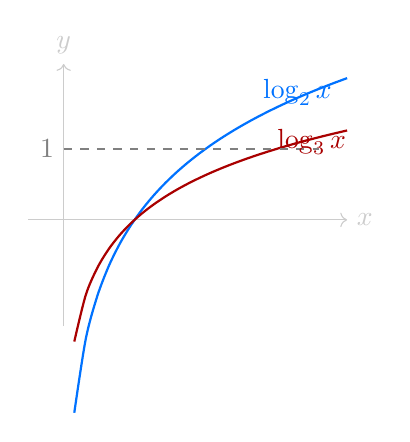
\begin{tikzpicture}[scale=0.9, baseline=(current bounding box.north)]
		\draw[->, gray!40] (-0.5,0) -- (4,0) node[right] {$x$};
		\draw[->, gray!40] (0,-1.5) -- (0,2.2) node[above] {$y$};
		\draw[thick, SkyBlue, domain=0.15:4, smooth, variable=\x] plot ({\x}, {ln(\x)/ln(2)});
		\draw[thick, DarkRed, domain=0.15:4, smooth, variable=\x] plot ({\x}, {ln(\x)/ln(3)});
		\draw[dashed, gray] (0,1) -- (3.6,1);
		\node[SkyBlue] at (3.3,1.8) {$\log_2 x$};
		\node[DarkRed] at (3.5,1.1) {$\log_3 x$};
		\node[left, gray] at (0,1) {$1$};
	\end{tikzpicture}
\end{center}

\category{求定义域}
\begin{question}
	$f(x)=\sqrt{x^2-3x-4}+\lg(6-x)$.
\end{question}

$x^2-3x-4\geq0 \implies x\leq-1$或$x\geq4$.

$6-x>0 \implies x<6$.

$\therefore (-\infty,-1]\cup[4,6)$.

\begin{knowledge}{比较大小}
	\begin{enumerate}[label=\arabic*., left=0pt]
		
		\item 同底不同真.
		
		\item 同真不同底.
		
		\item 真底均不同.
		
	\end{enumerate}
\end{knowledge}

\category{比较大小}
\begin{question}
	$\log_{\frac{1}{3}}\dfrac{1}{4}$与$\log_{1.5}\dfrac{2}{3}$.
\end{question}

$\log_{\frac{1}{3}}\dfrac{1}{4}=\log_3 4>1$；$\log_{1.5}\dfrac{2}{3}<0$.

$\therefore \log_{\frac{1}{3}}\dfrac{1}{4}>\log_{1.5}\dfrac{2}{3}$.

\begin{knowledge}{解不等式}
	换同底对数形式（利用单调性）.
	
	真数$>0$.
\end{knowledge}

\category{解不等式}
\begin{question}
	$\log_3 x>3$.
\end{question}

$\log_3 x>\log_3 3^3$.

$\therefore x>27$.

\category{底小于1}
\begin{question}
	$\log_{0.45}(x+2)<\log_{0.45}(1-x)$.
\end{question}

$x+2>0$，$1-x>0$，$x+2>1-x$（底$<1$，变号）.

$\therefore -\dfrac{1}{2}<x<1$.

\subsection{第十三讲\quad 图象变换与零点}

\subsubsection{图象变换}
\begin{knowledge}{变换}
	上下左右平移、点平移初中已学.
	
	翻折变换：
	$y=|f(x)|$：留上翻下.
	
	$y=f(|x|)$：去左称右.
\end{knowledge}

\category{分离常数}
\begin{question}
	$y=\dfrac{2x+4}{x}$（由$y=\dfrac{4}{x}$变换）.
\end{question}

$y=\dfrac{2x}{x}+\dfrac{4}{x}=\dfrac{4}{x}+2$.

$\therefore$ 由$y=\dfrac4x$上移$2$.

\category{翻折变换}
\begin{question}
	$y=x^2-2|x|$，即$y=|x|^2-2|x|$.
\end{question}

原图$y=x^2-2x$（轴$x=1$）$\Rightarrow$ 去左称右后轴$x=\pm1$.

\begin{center}
	\begin{tikzpicture}[scale=0.7, baseline=(current bounding box.north)]
		% 原图
		\begin{scope}[shift={(-4,0)}]
			\draw[->, gray!40] (-1.5,0) -- (3,0) node[right] {$x$};
			\draw[->, gray!40] (0,-1.5) -- (0,2.5) node[above] {$y$};
			\draw[thick, domain=-0.7:2.7, smooth, variable=\x] plot ({\x}, {(\x-1)*(\x-1)-1});
			\draw[dashed, gray] (1,-1.3) -- (1,2.3);
			\node[below] at (1,-1.4) {$x=1$};
			\node[above left] at (-0.8,2) {原图};
		\end{scope}
		\node at (0,0.5) {$\Rightarrow$};
		% 翻折后
		\begin{scope}[shift={(4,0)}]
			\draw[->, gray!40] (-3,0) -- (3,0) node[right] {$x$};
			\draw[->, gray!40] (0,-1.5) -- (0,2.5) node[above] {$y$};
			\draw[thick, domain=-2.6:2.6, smooth, variable=\x] plot ({\x}, {\x*\x-2*abs(\x)});
			\draw[dashed, gray] (1,-1.3) -- (1,2.3);
			\draw[dashed, gray] (-1,-1.3) -- (-1,2.3);
			\node[above] at (1,2.3) {$x=1$};
			\node[above] at (-1,2.3) {$x=-1$};
		\end{scope}
	\end{tikzpicture}
\end{center}

\subsubsection{零点问题}
\begin{knowledge}{方法}
	\begin{enumerate}[label=\arabic*., left=0pt]
		
		\item 解方程.
		
		\item 图象.
		
	\end{enumerate}
\end{knowledge}

\category{零点所在区间}
\begin{question}
	$f(x)=2^x+x^2-4$，判断零点所在区间：(1)$(-2,-1)$；(2)$(-1,0)$.
\end{question}

$f(-2)=\dfrac{1}{4}+4-4=\dfrac{1}{4}>0$；$f(-1)=\dfrac{1}{2}+1-4=-\dfrac{5}{2}<0$.

$\therefore$ 零点在$(-2,-1)$.

$f(0)=1-4=-3<0$，$f(-1)<0$，(2)不成立.

\subsection{第十四讲\quad 任意角的三角函数}

\subsubsection{任意角}
\begin{knowledge}{任意角}
	逆时针转角为正角；顺时针转角为负角；无旋转为零角.
	
	终边在坐标轴上的角不属于任何象限.
	
	终边在同一位置的角，角度差$360^\circ$.
	
	直线型：$\{\alpha|\alpha=\alpha_0+k\cdot180^\circ,\ k\in Z\}$.
	
	射线型：$\{\alpha|\alpha=\alpha_0+k\cdot360^\circ,\ k\in Z\}$.
\end{knowledge}

\subsubsection{弧度制}
\begin{knowledge}{弧度制}
	$\theta=\dfrac{l}{r}$；$\pi=180^\circ$.
	
	角度化弧度：乘$\dfrac{\pi}{180^\circ}$.
	
	弧度化角度：乘$\left(\dfrac{180}{\pi}\right)^\circ$.
\end{knowledge}

\subsubsection{任意角的三角函数}
\begin{knowledge}{定义与符号}
	$\sin\alpha=y$；$\cos\alpha=x$；$\tan\alpha=\dfrac{y}{x}$.
	
	符号：$\sin$一、二正，三、四负；$\cos$一、四正，二、三负；$\tan$一、三正，二、四负.
\end{knowledge}

\begin{center}
	\begin{tikzpicture}[scale=0.8, baseline=(current bounding box.north)]
		% 单位圆
		\begin{scope}[shift={(-6.5,0)}]
			\draw[->, gray!40] (-1.8,0) -- (1.8,0) node[right] {$x$};
			\draw[->, gray!40] (0,-1.8) -- (0,1.8) node[above] {$y$};
			\draw[thick] (0,0) circle (1.2);
			\draw[thick, DarkRed] (0,0) -- (0.85,0.85);
			\draw[dashed, SkyBlue] (0.85,0.85) -- (0,0.85);
			\draw[dashed, SkyBlue] (0.85,0.85) -- (0.85,0);
			\node[DarkRed] at (0.55,0.2) {$\alpha$};
		\end{scope}
		% sin 符号
		\begin{scope}[shift={(-3,0)}]
			\draw[->, gray!40] (-1.3,0) -- (1.3,0);
			\draw[->, gray!40] (0,-1.3) -- (0,1.3);
			\node at (0.6,0.6) {$+$};
			\node at (-0.6,0.6) {$+$};
			\node at (-0.6,-0.6) {$-$};
			\node at (0.6,-0.6) {$-$};
			\node[below] at (0,-1.4) {$\sin$};
		\end{scope}
		% cos 符号
		\begin{scope}[shift={(0,0)}]
			\draw[->, gray!40] (-1.3,0) -- (1.3,0);
			\draw[->, gray!40] (0,-1.3) -- (0,1.3);
			\node at (0.6,0.6) {$+$};
			\node at (-0.6,0.6) {$-$};
			\node at (-0.6,-0.6) {$-$};
			\node at (0.6,-0.6) {$+$};
			\node[below] at (0,-1.4) {$\cos$};
		\end{scope}
		% tan 符号
		\begin{scope}[shift={(3,0)}]
			\draw[->, gray!40] (-1.3,0) -- (1.3,0);
			\draw[->, gray!40] (0,-1.3) -- (0,1.3);
			\node at (0.6,0.6) {$+$};
			\node at (-0.6,0.6) {$-$};
			\node at (-0.6,-0.6) {$+$};
			\node at (0.6,-0.6) {$-$};
			\node[below] at (0,-1.4) {$\tan$};
		\end{scope}
	\end{tikzpicture}
\end{center}

\subsection{第十五讲\quad 同角基本关系与诱导公式}

\subsubsection{同角基本关系}
\begin{knowledge}{同角基本关系}
	$\sin^2\alpha+\cos^2\alpha=1$.
	
	$\dfrac{\sin\alpha}{\cos\alpha}=\tan\alpha$.
	
	技巧：画图；定号.
	
	计算方法：
	\begin{enumerate}[label=\arabic*., left=0pt]
		
		\item 猛算出$\cos\alpha,\sin\alpha$.
		
		\item 用$\tan\alpha=\dfrac{\sin\alpha}{\cos\alpha}=$常数$\implies\sin\alpha=x\cos\alpha$套入，化切为弦.
		
		\item 上下同除$\cos\alpha$或$\cos^2\alpha$，化弦为切.
		
	\end{enumerate}
\end{knowledge}

\subsubsection{诱导公式}
\begin{knowledge}{使用步骤}
	\begin{enumerate}[label=\arabic*., left=0pt]
		
		\item 公式1：加减整数$2\pi\to[-\pi,\pi]$.
		
		\item 看能否用其他公式.
		
		\item 如不可，用公式3提负号.
		
	\end{enumerate}
\end{knowledge}

\begin{knowledge}{12个诱导公式}
	\begin{enumerate}[label=\arabic*., left=0pt]
		
		\item $\sin(2k\pi+\alpha)=\sin\alpha$.
		
		\item $\cos(2k\pi+\alpha)=\cos\alpha$.
		
		\item $\sin(\pi+\alpha)=-\sin\alpha$.
		
		\item $\cos(\pi+\alpha)=-\cos\alpha$.
		
		\item $\sin(-\alpha)=-\sin\alpha$.
		
		\item $\cos(-\alpha)=\cos\alpha$.
		
		\item $\sin(\pi-\alpha)=\sin\alpha$.
		
		\item $\cos(\pi-\alpha)=-\cos\alpha$.
		
		\item $\sin\left(\dfrac{\pi}{2}-\alpha\right)=\cos\alpha$.
		
		\item $\cos\left(\dfrac{\pi}{2}-\alpha\right)=\sin\alpha$.
		
		\item $\sin\left(\dfrac{\pi}{2}+\alpha\right)=\cos\alpha$.
		
		\item $\cos\left(\dfrac{\pi}{2}+\alpha\right)=-\sin\alpha$.
		
	\end{enumerate}
	
	附：$\tan(2k\pi+\alpha)=\tan\alpha$；$\tan(\pi+\alpha)=\tan\alpha$；$\tan(-\alpha)=-\tan\alpha$；$\tan(\pi-\alpha)=-\tan\alpha$.
\end{knowledge}



\section{高一上学期秋季}












\section{准高二暑期数学}

\subsection{第一讲\quad 空间向量的概念及其运算}

\subsubsection{空间向量的概念及其线性运算}

\begin{knowledge}{共面向量定理}
	$\overrightarrow{a}$与$\overrightarrow{b}$不共线，则向量$\overrightarrow{p}$与向量$\overrightarrow{a},\overrightarrow{b}$共面的充要条件是存在唯一一对实数$x,y$，使
	\[
	\overrightarrow{p}=x\overrightarrow{a}+y\overrightarrow{b}
	\]
	\textbf{用途：证明向量共面}
	
	$\overrightarrow{OP}=x\overrightarrow{OA}+y\overrightarrow{OB}+z\overrightarrow{OC}$，$x+y+z=1$.
	
	$\implies ABCP$四点共面.
	
	\textbf{技巧：系数大的放左边}
\end{knowledge}

\category{思维延伸}
\begin{question}
	已知$M,N$，若$\overrightarrow{OG}=\dfrac{1}{3}\overrightarrow{OA}+x\overrightarrow{OB}+y\overrightarrow{OC}$，且$G,M,N$三点共线，求$x+y$.
\end{question}

\begin{minipage}[t]{0.5\textwidth}
	由$G,M,N$共线：
	\[
	\overrightarrow{OG}=m\overrightarrow{OM}+(1-m)\overrightarrow{ON}
	\]
	依题意，将$\overrightarrow{OM},\overrightarrow{ON}$转化为$\overrightarrow{OA},\overrightarrow{OB},\overrightarrow{OC}$表示：
	\[
	\overrightarrow{OG}=\dfrac{1}{3}m\overrightarrow{OA}+(1-m)\cdot \dfrac{1}{2}(\overrightarrow{OB}+\overrightarrow{OC})
	\]
	\[
	\dfrac{1}{3}m=\dfrac{1}{3} \implies m=\dfrac{2}{3}
	\]
	\[
	\therefore \overrightarrow{OG}=\dfrac{2}{9}\overrightarrow{OA}+\dfrac{1}{6}\overrightarrow{OB}+\dfrac{1}{6}\overrightarrow{OC}
	\]
	\[
	\therefore x+y=\dfrac{1}{6}+\dfrac{1}{6}=\dfrac{1}{3}
	\]
\end{minipage}
\hfill
\begin{minipage}[t]{0.4\textwidth}
	\centering
	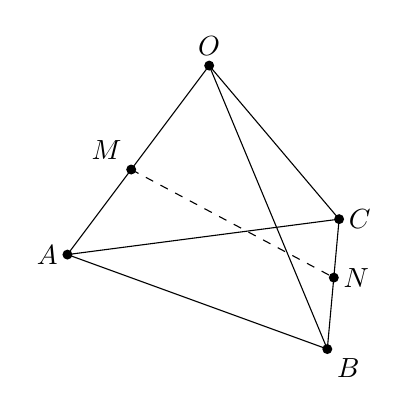
\begin{tikzpicture}[scale=1.5,baseline=(current bounding box.north)]
		\coordinate (A) at (-1.2,0);
		\coordinate (B) at (1,-0.8);
		\coordinate (C) at (1.1,0.3);
		\coordinate (O) at (0,1.6);
		\coordinate (M) at ($(A)!0.45!(O)$);
		\coordinate (N) at ($(B)!0.55!(C)$);
		\draw (A)--(B)--(C)--cycle;
		\draw (O)--(A); \draw (O)--(B); \draw (O)--(C);
		\draw[dashed] (M)--(N);
		\fill (A) circle (1.2pt) node[left] {$A$};
		\fill (B) circle (1.2pt) node[below right] {$B$};
		\fill (C) circle (1.2pt) node[right] {$C$};
		\fill (O) circle (1.2pt) node[above] {$O$};
		\fill (M) circle (1.2pt) node[above left] {$M$};
		\fill (N) circle (1.2pt) node[right] {$N$};
	\end{tikzpicture}
\end{minipage}

\category{向量共面}
\begin{question}
	已知$\overrightarrow{p}=2\overrightarrow{a}-\overrightarrow{b}+2\overrightarrow{c},\quad
	\overrightarrow{q}=-\overrightarrow{a}+3\overrightarrow{b}-3\overrightarrow{c},\quad
	\overrightarrow{r}=13\overrightarrow{a}+6\overrightarrow{b}+\lambda\overrightarrow{c}
	$若$\overrightarrow{p},\overrightarrow{q},\overrightarrow{r}$共面，则$\lambda=$?
\end{question}
三向量共面：
\[
13\overrightarrow{a}+6\overrightarrow{b}+\lambda\overrightarrow{c}=x\left(2\overrightarrow{a}-\overrightarrow{b}+2\overrightarrow{c}\right)+y\left(-\overrightarrow{a}+3\overrightarrow{b}-3\overrightarrow{c}\right)
\]
整理右侧：
\[
13\overrightarrow{a}+6\overrightarrow{b}+\lambda\overrightarrow{c}
=(2x-y)\overrightarrow{a}+(-x+3y)\overrightarrow{b}+(2x-3y)\overrightarrow{c}
\]
由向量相等，对应系数相等建立方程组：
\[
\begin{cases}
	2x-y=13\\
	-x+3y=6\\
	\lambda=2x-3y
\end{cases}
\]
解得：$x=9,\;y=5$，代入得 $\lambda=3$.

\category{四点共面}
\begin{question}{}
	$A,B,C,D$四点共面，且$\overrightarrow{DP}=m\overrightarrow{OA}+\overrightarrow{OB}+\overrightarrow{OC}$，求$m=$？
\end{question}
四点共面结论：起点一样，则向量系数之和为$1$.
\[
\begin{aligned}
	\overrightarrow{OP}-\overrightarrow{OB}&=m\overrightarrow{OA}+\overrightarrow{OB}+\overrightarrow{OC} \\
	\overrightarrow{OP}&=m\overrightarrow{OA}+2\overrightarrow{OB}+\overrightarrow{OC}
\end{aligned}
\]
\[
m+2+1=1 \implies m=-2
\]

\subsubsection{向量的数量积}
\begin{knowledge}{投影相关公式}
	投影：$|\overrightarrow{b}|\cdot\cos\langle\overrightarrow{a},\overrightarrow{b}\rangle$
	
	投影向量：$\displaystyle |\overrightarrow{b}|\cdot\cos\langle\overrightarrow{a},\overrightarrow{b}\rangle\cdot\frac{\overrightarrow{a}}{|\overrightarrow{a}|}$
\end{knowledge}

\begin{question}{}
	已知$AB=4,AD=3,AA'=3$，$\angle BAD=90^\circ$，$\angle BAA'=60^\circ$，$\angle DAA'=60^\circ$，求$|AC'|$.
\end{question}

\begin{minipage}[t]{0.5\textwidth}
	\[
	\begin{aligned}
		|\overrightarrow{AC'}|&=\sqrt{(\overrightarrow{AB}+\overrightarrow{AD}+\overrightarrow{AA'})^2} \\
		&=\sqrt{|\overrightarrow{AB}|^2+|\overrightarrow{AD}|^2+|\overrightarrow{AA'}|^2
			+2\overrightarrow{AB}\cdot\overrightarrow{AD}+2\overrightarrow{AD}\cdot\overrightarrow{AA'}+2\overrightarrow{AB}\cdot\overrightarrow{AA'}} \\
		&=\sqrt{4^2+3^2+3^2+0+9+12} \\
		&=\sqrt{55}
	\end{aligned}
	\]
\end{minipage}
\hfill
\begin{minipage}[t]{0.3\textwidth}
	\centering
	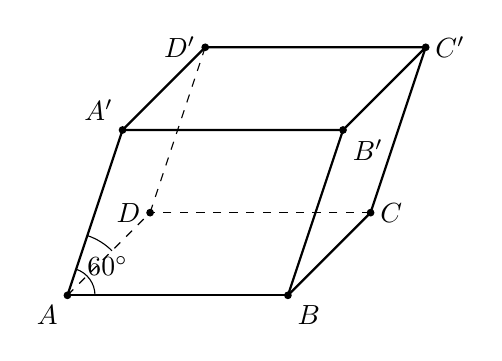
\begin{tikzpicture}[scale=0.7,baseline=(current bounding box.north)]
		% 命名点
		\coordinate (A) at (0,0);
		\coordinate (B) at (4,0);
		\coordinate (C) at (5.5,1.5);
		\coordinate (D) at (1.5,1.5);
		\coordinate (A') at (1,3);
		\coordinate (B') at (5,3);
		\coordinate (C') at (6.5,4.5);
		\coordinate (D') at (2.5,4.5);
		
		% 用括号括起所有坐标名
		\draw[thick] (A) -- (B);
		\draw[thick] (B) -- (C);
		\draw[dashed] (A) -- (D);
		\draw[dashed] (C) -- (D);
		\draw[thick] (A') -- (B') -- (C') -- (D') -- cycle;
		\draw[thick] (A) -- (A');
		\draw[thick] (B) -- (B');
		\draw[thick] (C) -- (C');
		\draw[dashed] (D) -- (D');
		
		% 批量标记所有点
		\foreach \p/\pos in {A/below left,B/below right,C/right,D/left,A'/above left,B'/below right,C'/right,D'/left}
		\fill (\p) circle (2pt) node[\pos] {$\p$};
		\draw pic["$60^\circ$", draw, angle eccentricity=1.8, angle radius=0.35cm] 
		{angle = B--A--A'};
		\draw pic["", draw, angle eccentricity=2.5, angle radius=0.8cm] 
		{angle = D--A--A'};
	\end{tikzpicture}
\end{minipage}

\subsubsection{坐标运算}
\begin{question}{}
	若$A(m+1,n+1,3),\,B(2m,n,m-2n),\,C(m+3,n-3,9)$三点共线，则$m+n=$？
\end{question}
\[
\overrightarrow{AB}=(m-1,-1,m-2n-3),\quad \overrightarrow{AC}=(2,-4,6)
\]
三点共线：$\overrightarrow{AB}=\lambda\overrightarrow{AC}$，由$y$分量可知 $\lambda=\dfrac{1}{4}$.
\[
\begin{cases}
	\dfrac{2}{4}=m-1 \\
	\dfrac{6}{4}=m-2n-3
\end{cases}
\implies
\begin{cases}
	m=\dfrac{3}{2}\\[4pt]
	n=-\dfrac{3}{2}
\end{cases}
\implies m+n=0
\]

\begin{question}
	已知点$A(2,-1,7)$，向量$\overrightarrow{a}=(18,9,-12)$，$\overrightarrow{AB}\parallel\overrightarrow{a}$，线段长$|AB|=34$，求$B$点坐标.
\end{question}

$\overrightarrow{AB}\parallel\overrightarrow{a}\implies \overrightarrow{AB}=\lambda\overrightarrow{a}\ (\lambda>0)$

设$B(x,y,z)$

$(x-2,y+1,z-7)=\lambda(18,9,-12)$

$\sqrt{(18\lambda)^2+(9\lambda)^2+(-12\lambda)^2}=34 \implies \lambda=2$

$\therefore B=(38,17,-17)$

\subsection{第二讲\quad 立体几何中的向量方法}

\subsubsection{方向向量与法向量}
\begin{knowledge}{基本定义}
	直线的方向向量：$A,B$ 为直线上不同两点，则与 $\overrightarrow{AB}$ 平行的向量称为直线的方向向量.
	
	平面的法向量：若 $\boldsymbol{n}\perp$ 平面，则与 $\boldsymbol{n}$ 平行的非零向量为平面法向量.
\end{knowledge}

\begin{knowledge}{法向量标准求解步骤}
	\begin{enumerate}[label=\bfseries\arabic*.]
		\item 建立空间直角坐标系，写出点坐标；
		\item 求出平面内两条相交边对应的方向向量；
		\item 设法向量 $\boldsymbol{n}=(x,y,z)$，列数量积为0的方程组；
		\item 赋值，解方程组得到一组法向量.
	\end{enumerate}
\end{knowledge}
以一点为原点，三条两两垂直的方向分别作为坐标轴，建立空间直角坐标系.

\category{正方体求法向量}
\begin{question}
	正方体棱长为3，设 $A(3,0,0),\,E(3,3,1),\,F(0,3,2)$，求平面$AEF$的一个法向量.
\end{question}

\begin{minipage}[t]{0.5\textwidth}
	$\overrightarrow{AE}=(0,3,1),\quad \overrightarrow{FE}=(3,0,-1)$
	
	设平面$AEF$的一个法向量为 $\boldsymbol{n}=(x,y,z)$，满足
	\[
	\begin{cases}
		\boldsymbol{n}\cdot\overrightarrow{AE}=0\\
		\boldsymbol{n}\cdot\overrightarrow{FE}=0
	\end{cases}
	\implies
	\begin{cases}
		3y+z=0\\
		3x-z=0
	\end{cases}
	\]
	令 $z=3$，得 $x=1,\,y=-1$，可取 $\boldsymbol{n}=(1,-1,3)$.
\end{minipage}
\hfill
\begin{minipage}[t]{0.34\textwidth}
	\tdplotsetmaincoords{70}{110}
	\begin{tikzpicture}[baseline=(current bounding box.north), scale=1
		,tdplot_main_coords
		]
		% 坐标点定义
		\coordinate (D) at (0,0,0);
		\coordinate (A) at (3,0,0);
		\coordinate (B) at (3,3,0);
		\coordinate (C) at (0,3,0);
		\coordinate (D1) at (0,0,3);
		\coordinate (A1) at (3,0,3);
		\coordinate (B1) at (3,3,3);
		\coordinate (C1) at (0,3,3);
		
		% 三等分点 E 和 F
		\coordinate (E) at (3,3,1); % E 在 BB1 上
		\coordinate (F) at (0,3,2); % F 在 CC1 上
		
		% 坐标轴 (内部虚线，外部实线)
		\draw[->, dashed] (D) -- (A);
		\draw[->, thick] (A) -- (4.5,0,0) node[below] {$x$};
		\draw[->, dashed] (D) -- (C);
		\draw[->, thick] (C) -- (0,4.5,0) node[right] {$y$};
		\draw[->, dashed] (D) -- (D1);
		\draw[->, thick] (D1) -- (0,0,4.5) node[above] {$z$};
		
		% 正方体可见边
		\draw[thick] (A) -- (B) -- (C);
		\draw[thick] (A) -- (A1);
		\draw[thick] (B) -- (B1);
		\draw[thick] (C) -- (C1);
		\draw[thick] (A1) -- (B1) -- (C1) -- (D1) -- cycle;
		
		% 顶点标签
		\node[left] at (A) {$A$};
		\node[right] at (B) {$B$};
		\node[below right] at (C) {$C$};
		\node[left] at (D) {$D$};
		\node[left] at (A1) {$A_1$};
		\node[right] at (B1) {$B_1$};
		\node[above right] at (C1) {$C_1$};
		\node[left] at (D1) {$D_1$};
		
		% 平面 AEF (可见边界为实线，不可见为虚线)
		\draw[thick, dashed] (A) -- (F); % 穿过体内部
		\draw[thick] (A) -- (E);         % 前面
		\draw[thick] (E) -- (F);         % 右侧面
		
		% 标注 E, F 点
		\node[right] at (E) {$E$};
		\node[right] at (F) {$F$};
		\fill (E) circle (1.5pt);
		\fill (F) circle (1.5pt);
	\end{tikzpicture}
\end{minipage}

\subsubsection{空间平行、垂直与空间向量的关系}

\begin{knowledge}{平行、垂直判定结论}
	\begin{itemize}
		\item 线$\parallel$线 $\iff$ 方向向量互相平行；线$\perp$线 $\iff$ 方向向量互相垂直
		\item 线$\parallel$面 $\iff$ 直线方向向量与平面法向量垂直；线$\perp$面 $\iff$ 直线方向向量与平面法向量平行
		\item 面$\parallel$面 $\iff$ 两平面法向量互相平行；面$\perp$面 $\iff$ 两平面法向量互相垂直
	\end{itemize}
	
	可画图确认
\end{knowledge}

\category{正方体证明线面垂直}
\begin{question}{正方体线面平行证明}
	正方体，$E$为$BC$中点，$F$为$CD$中点，$G$为$C_1D_1$中点，求证：$BG\parallel$ 平面$EFC_1$.
\end{question}
\begin{minipage}[t]{0.7\textwidth}
	设正方体棱长为$2$，以$C$为原点，$CB,CD,CC_1$分别为$x,y,z$轴建系：
	\[
	C(0,0,0), B(2,0,0), D(0,2,0), C_1(0,0,2), D_1(0,2,2)
	\]
	\[
	E(1,0,0), F(0,1,0), G(0,1,2)
	\]
	\[
	\overrightarrow{FE}=(1,-1,0), \overrightarrow{FC_1}=(0,-1,2)
	\]
	设平面$EFC_1$法向量$\boldsymbol{n}=(x,y,z)$
	\[
	\begin{cases}
		\boldsymbol{n}\cdot\overrightarrow{FE}=x-y=0\\
		\boldsymbol{n}\cdot\overrightarrow{FC_1}=-y+2z=0
	\end{cases}
	\Rightarrow x=y=2z,\text{取}z=1,\boldsymbol{n}=(2,2,1)
	\]
	\[
	\overrightarrow{BG}=(-2,1,2)
	\]
	\[
	\overrightarrow{BG}\cdot\boldsymbol{n}=2\times(-2)+2\times1+1\times2=0
	\]
	又$BG\not\subset$平面$EFC_1$，故$BG\parallel$平面$EFC_1$.
\end{minipage}
\hfill
\begin{minipage}[t]{0.5\textwidth}
	\tdplotsetmaincoords{70}{110}
	\begin{tikzpicture}[baseline=(current bounding box.north), scale=1,tdplot_main_coords]
		\coordinate (C) at (0,0,0);
		\coordinate (B) at (2,0,0);
		\coordinate (D) at (0,2,0);
		\coordinate (A) at (2,2,0);
		\coordinate (C1) at (0,0,2);
		\coordinate (B1) at (2,0,2);
		\coordinate (D1) at (0,2,2);
		\coordinate (A1) at (2,2,2);
		\coordinate (E) at (1,0,0);
		\coordinate (F) at (0,1,0);
		\coordinate (G) at (0,1,2);
		
		\draw[->, dashed] (C)--(B);
		\draw[->, thick] (B)--(3,0,0) node[below]{$x$};
		\draw[->, dashed] (C)--(D);
		\draw[->, thick] (D)--(0,3,0) node[right]{$y$};
		\draw[->, dashed] (C)--(C1);
		\draw[->, thick] (C1)--(0,0,3) node[above]{$z$};
		
		\draw[thick] (A)--(B)--(C)--(D)--cycle;
		\draw[thick] (A1)--(B1)--(C1)--(D1)--cycle;
		\draw[thick] (A)--(A1) (B)--(B1) (D)--(D1);
		\draw[thick, SkyBlue] (E)--(F)--(C1)--cycle;
		\draw[thick, red] (B)--(G);
		
		\node[below right] at (A) {$A$};
		\node[left] at (B) {$B$};
		\node[left] at (C) {$C$};
		\node[below] at (D) {$D$};
		\node[right] at (A1) {$A_1$};
		\node[left] at (B1) {$B_1$};
		\node[left] at (C1) {$C_1$};
		\node[right] at (D1) {$D_1$};
		\fill (E) circle (1.5pt) node[below]{$E$};
		\fill (F) circle (1.5pt) node[below left]{$F$};
		\fill (G) circle (1.5pt) node[above left]{$G$};
	\end{tikzpicture}
\end{minipage}

\subsubsection{角度问题}
\begin{knowledge}{三类空间角向量公式}
	\begin{itemize}
		\item 线线角：$\cos\theta=\left|\cos\langle \overrightarrow{v_1},\overrightarrow{v_2}\rangle\right|$
		\item 线面角：$\sin\theta=\left|\cos\langle \overrightarrow{v},\boldsymbol{n}\rangle\right|$，$\overrightarrow{v}$ 为直线方向向量，$\boldsymbol{n}$ 为平面法向量
		\item 面面角：$|\cos\theta|=\left|\cos\langle \boldsymbol{n_1},\boldsymbol{n_2}\rangle\right|$，$\boldsymbol{n_1},\boldsymbol{n_2}$ 为两平面法向量
	\end{itemize}
\end{knowledge}

\category{长方体求线面角}
\begin{question}
	$AB=AA_1=2, AD=4$, $M$是$A_1B_1$中点
	
	(1) $BC$与平面$BMD_1$是所成角的正弦值
	
	(2) $\angle B-MD_1-B_1$的余弦值
\end{question}

\begin{minipage}[t]{0.5\textwidth}
	\begin{enumerate}[label=(\arabic*)]
		\item $\overrightarrow{BC}$的方向向量为$\overrightarrow{v}=(0,1,0)$
		
		$\overrightarrow{n}=(4,1,-2)$
		
		$\sin \theta =|cos\langle\overrightarrow{v},\overrightarrow{n}\rangle|=\dfrac{\sqrt{21}}{21}$
		\item $\overrightarrow{n}'=(0,0,1)$
		
		$|\cos\theta| = |\cos\langle\overrightarrow{n},\overrightarrow{n}'\rangle|=\dfrac{2\sqrt{21}}{21}$
		
		$\therefore \angle B-MD_1-B_1$的余弦值为$\dfrac{2\sqrt{21}}{21}$ 
	\end{enumerate}
	
	
\end{minipage}
\hfill
\begin{minipage}[t]{0.4\textwidth}
	\tdplotsetmaincoords{70}{110}
	\begin{tikzpicture}[baseline=(current bounding box.north), scale=1,tdplot_main_coords]
		% 长方体坐标，A在上，A1在下，AB=2, AA1=2, AD=4
		\coordinate (A) at (0,0,2);
		\coordinate (B) at (2,0,2);
		\coordinate (D) at (0,4,2);
		\coordinate (C) at (2,4,2);
		\coordinate (A1) at (0,0,0);
		\coordinate (B1) at (2,0,0);
		\coordinate (D1) at (0,4,0);
		\coordinate (C1) at (2,4,0);
		% M 为 A1B1 中点
		\coordinate (M) at ($(A1)!0.5!(B1)$);
		
		% 坐标轴
		\draw[->, dashed] (A1) -- (B1);
		\draw[->, thick] (B1) -- (3,0,0) node[below] {$x$};
		\draw[->, dashed] (A1) -- (D1);
		\draw[->, thick] (D1) -- (0,5,0) node[right] {$y$};
		\draw[->, dashed] (A1) -- (A);
		\draw[->, thick] (A) -- (0,0,3) node[above] {$z$};
		
		% 长方体棱 实线可见
		\draw[thick] (A)--(B)--(C)--(D)--cycle;
		\draw[thick] (A1)--(B1)--(C1)--(D1)--cycle;
		\draw[thick] (A)--(A1);
		\draw[thick] (B)--(B1);
		\draw[thick] (C)--(C1);
		\draw[thick] (D)--(D1);
		
		% 目标平面 BMD1 线条
		\draw[thick] (B)--(M);
		\draw[thick] (M)--(D1);
		\draw[thick] (B)--(D1);
		\draw[thick] (M)--(B1);
		
		% 顶点标注
		\node[above left] at (A) {$A$};
		\node[above left] at (B) {$B$};
		\node[above] at (D) {$D$};
		\node[above] at (C) {$C$};
		\node[above left] at (A1) {$A_1$};
		\node[left] at (B1) {$B_1$};
		\node[below] at (D1) {$D_1$};
		\node[below] at (C1) {$C_1$};
		\node[left] at (M) {$M$};
		
		% 标记特殊点
		\fill (M) circle (1.5pt);
	\end{tikzpicture}
\end{minipage}

\subsection{第三讲\quad 直线方程}
\subsubsection{直线方程}
\begin{knowledge}{直线方程（五类方程）}
	倾斜角：$l$向上方向与$x$正方向夹角
	斜率 $k=\tan\alpha=\dfrac{y_2-y_1}{x_2-x_1}$
	
	技巧：注意$k>0$是否在题目范围内；倾斜角需要分类讨论
	\begin{enumerate}[label=\bfseries\arabic*.]
		\item 点斜式方程：$y-y_0=k(x-x_0)$ \quad[一个点+ $k$] \quad \textbf{不能表示垂直$x$轴直线}
		\item 斜截式方程：$y=kx+b$，$b$为纵截距 \quad [纵截距+ $k$] \quad \textbf{不能表示$\alpha=90^\circ$}
		\item 两点式方程 \quad [求$k$+点斜式]
		\item 截距式方程：过$(a,0)$和$(0,b)$，$\dfrac{x}{a}+\dfrac{y}{b}=1$
		\quad \textbf{不能表示横、竖直线，不能表示过原点直线}
		\item 一般式方程 $Ax+By+C=0$（不轻易用）
	\end{enumerate}
\end{knowledge}

\category{关于截距}
\begin{question}
	经过$(1,2)$且两截距绝对值相等的直线方程为?
\end{question}

题目涉及截距，优先考虑截距式，分类讨论：
\begin{enumerate}[label=\arabic*.]
	\item 直线过原点：$y=2x$
	\item 直线不过原点，不是横竖直线
	\begin{enumerate}[label=(\arabic*)]
		\item $a=b$，$\dfrac{x}{a}+\dfrac{y}{a}=1$，代入$(1,2)$，得$a=3$，方程：$x+y-3=0$
		\item $a=-b$，$\dfrac{x}{a}-\dfrac{y}{a}=1$，代入$(1,2)$，得$a=-1$，方程：$-x+y=1$
	\end{enumerate}
\end{enumerate}

\subsubsection{位置关系与距离公式}
\begin{knowledge}{位置关系与距离公式}
	对于一般式 $A_1x+B_1y+C_1=0,\ A_2x+B_2y+C_2=0$
	\begin{itemize}
		\item 平行：$\dfrac{A_1}{A_2}=\dfrac{B_1}{B_2}\neq\dfrac{C_1}{C_2}$，注意排除重合直线
		\item 垂直：$A_1A_2+B_1B_2=0$
	\end{itemize}
	
	点到直线距离：$\displaystyle d=\dfrac{|Ax_0+By_0+C|}{\sqrt{A^2+B^2}}$
	
	两平行线距离：$\displaystyle d=\dfrac{|C_1-C_2|}{\sqrt{A^2+B^2}}$
	先将$x,y$系数统一再求C！
	
	圆锥曲线大题意识：看到带参数的直线方程，表明直线过定点.
\end{knowledge}

\category{直线平行判定}
\begin{question}
	设$m\in\mathbb{R}$，则$m=-3$是直线$mx+3y=2-m$与$x+(m+1)y=1$平行的什么条件？
\end{question}

平行条件：$\dfrac{A_1}{A_2}=\dfrac{B_1}{B_2}\neq\dfrac{C_1}{C_2}$
\[
\dfrac{m}{1}=\dfrac{3}{m+1}\implies m=-3 \text{ 或 }m=2
\]
当$m=2$时，两条直线方程相同，为重合，舍去.\newline
故为充要条件.

\category{点线距}
\begin{question}
	直线过$(-1,2)$，原点到直线距离为$1$，求直线方程
\end{question}
\begin{enumerate}[label=\arabic*.]
	\item 直线垂直$x$轴：$x=-1$
	\item 直线不垂直$x$轴，设斜率$k$
	\[
	y-2=k(x+1)\implies kx-y+k+2=0
	\]
	\[
	d=\dfrac{|k+2|}{\sqrt{k^2+1}}=1,\quad |k+2|=\sqrt{k^2+1}
	\]
	解得 $k=-\dfrac{3}{4}$，直线方程：$3x+4y-5=0$
\end{enumerate}

\category{线线距}
\begin{question}
	两条平行直线$3x+4y-12=0$与$ax+8y+11=0$之间的距离为?
\end{question}

平行直线满足：$\dfrac{3}{a}=\dfrac{4}{8}$，解得$a=6$.

前提：$A,B$系数统一，第一个方程左右同乘$2$：$6x+8y-24=0$，此时$A=6,B=8,C_1=-24,C_2=11$.
\[
d=\dfrac{|-24-11|}{\sqrt{6^2+8^2}}=\dfrac{35}{10}=\dfrac{7}{2}.
\]

\category{斜率取值范围}
\begin{question}
	过原点的直线$l$的倾斜角取值范围为$\left[\dfrac{\pi}{3},\dfrac{3\pi}{4}\right]$，则其斜率的取值范围?
\end{question}

\begin{minipage}[t]{0.7\textwidth}
	
	$\tan\dfrac{\pi}{3}=\sqrt{3},\ \tan\dfrac{3\pi}{4}=-1$.
	
	由图像可得斜率范围：$(-\infty,-1]\cup[\sqrt{3},+\infty)$.
\end{minipage}
\hfill
\begin{minipage}[t]{0.3\textwidth}
	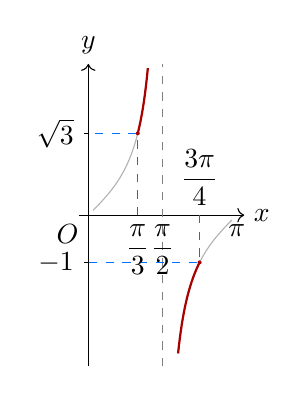
\begin{tikzpicture}[scale=0.6,baseline=(current bounding box.north)]
		\draw[->] (-0.2,0)--(3.3,0) node[right]{$x$};
		\draw[->] (0,-3.2)--(0,3.2) node[above]{$y$};
		
		% 仅标记关键y值
		\draw (0,-1)--(-0.1,-1) node[left] {$-1$};
		\draw (0,{sqrt(3)})--(-0.1,{sqrt(3)}) node[left] {$\sqrt{3}$};
		
		% tanx 只画 [0, pi] 一个周期，远离pi/2渐近线
		\draw[gray!60] plot[domain=0.1:1.26] (\x,{tan(deg(\x))});
		\draw[gray!60] plot[domain=1.9:3.04] (\x,{tan(deg(\x))});
		
		%目标区间红线
		\draw[DarkRed,thick] plot[domain={pi/3}:1.26] (\x,{tan(deg(\x))});
		\draw[DarkRed,thick] plot[domain=1.9:{3*pi/4}] (\x,{tan(deg(\x))});
		
		%渐近线虚线 x=π/2
		\draw[dashed,gray] (pi/2,-3.2)--(pi/2,3.2);
		
		%辅助虚线
		\draw[dashed,SkyBlue] (pi/3,0)--(pi/3,{sqrt(3)})--(0,{sqrt(3)});
		\draw[dashed,SkyBlue] (3*pi/4,0)--(3*pi/4,-1)--(0,-1);
		
		%关键点标记
		\fill[DarkRed] (pi/3,{sqrt(3)}) circle (1.2pt);
		\fill[DarkRed] (3*pi/4,-1) circle (1.2pt);
		
		%刻度，3π/4保留above避免图像遮挡
		\node[below] at (pi/3,0) {$\dfrac{\pi}{3}$};
		\node[below] at (pi/2,0) {$\dfrac{\pi}{2}$};
		\node[above] at (3*pi/4,0) {$\dfrac{3\pi}{4}$};
		\node[below] at (pi,0) {$\pi$};
		\node[below left] at (0,0) {$O$};
	\end{tikzpicture}
\end{minipage}

\category{过定点}
\begin{question}
	$(2k-1)x-(k+3)y-(k-11)=0$过定点?
\end{question}

整理式子：
\[
k(2x-y-1)-x-3y+11=0
\]
联立方程组
\[
\begin{cases}
	2x-y-1=0\\
	-x-3y+11=0
\end{cases}
\]
解得$\begin{cases}x=2\\y=3\end{cases}$，直线过定点$(2,3)$.

\subsection{第四讲\quad 直线与圆}
\category{圆的方程、点、线、圆与圆的位置关系}

\subsubsection{圆的方程}
\begin{knowledge}{}
	以$(a,b)$为圆心、$r$为半径的圆的标准方程：
	\[
	(x-a)^2+(y-b)^2=r^2
	\]
	圆心坐标：$(a,b)$.
	
	圆的一般方程：$x^2+y^2+Dx+Ey+F=0$
	\begin{enumerate}
		\item $x^2$、$y^2$项系数相等且不为$0$；
		\item 圆心坐标为$\left(-\dfrac{D}{2},-\dfrac{E}{2}\right)$，半径为$\dfrac12\sqrt{D^2+E^2-4F}$；
		\item 只有$x^2$、$y^2$系数为$1$，才可直接读取参数$D,E,F$；
		\item $D^2+E^2-4F>0$，方程才表示圆.
	\end{enumerate}
	已知圆上三点，可列三元一次方程组求解圆方程.
\end{knowledge}

\subsubsection{点、直线、圆与圆的位置关系}
\begin{knowledge}{}
	\begin{enumerate}
		\item 点与圆：将点代入圆方程，结果与$r^2$比较大小.
		\item 直线与圆
		\begin{enumerate}
			\item 计算圆心到直线距离，与半径比较；
			\item 联立直线与圆方程，消元得到一元二次方程，通过判别式$\Delta$判定位置.
		\end{enumerate}
		\item 圆与圆：计算两圆圆心距，和$|r_1-r_2|$、$r_1+r_2$比较.
	\end{enumerate}
	
	内含：$d<|r_1-r_2|$
	
	内切：$d=|r_1-r_2|$
	
	相交：$|r_1-r_2|<d<r_1+r_2$
	
	外切：$d=r_1+r_2$
	
	外离：$d>r_1+r_2$
\end{knowledge}

\begin{question}{例题1}
	方程$a^2x^2+(a+2)y^2+4x+8y+5a=0$表示圆，求该圆的圆心.
\end{question}

解：
圆方程中$x^2,y^2$系数相等
\[
a^2 = a+2 \implies a=2 \text{ 或 } a=-1
\]
当$a=2$，代入得
\[
4x^2+4y^2+4x+8y+10=0
\]
\[
x^2+y^2+x+2y+\frac52=0
\]
$D^2+E^2-4F<0$，不表示圆，舍去.

当$a=-1$，满足条件，圆心为$(-2,-4)$.

\vspace{6pt}
\begin{question}{例题2}
	直线$3x+4y+m=0$与圆$x^2+y^2-2x+4y+1=0$相切，求$m$的值.
\end{question}

圆$x^2+y^2-2x+4y+1=0$圆心$(1,-2)$，半径$r=2$.
\[
d=\frac{|3-8+m|}{5}=2 \implies m=-5 \text{ 或 } m=15
\]

\vspace{6pt}
\begin{question}{例题3}
	半径为$\sqrt2$，且与圆$x^2+y^2+10x+10y=0$外切于原点，求该圆的标准方程.
\end{question}

\begin{minipage}[t]{0.7\textwidth}
	解：
	圆$x^2+y^2+10x+10y=0$圆心$(-5,-5)$，半径$5\sqrt2$.
	
	两圆外切于原点，则所求圆圆心在直线$y=x$上，设圆心$(m,m)$.
	\[
	\sqrt{2(m+5)^2}=6\sqrt2 \implies m=1
	\]
	圆心$(1,1)$，半径$\sqrt2$.
	\[
	(x-1)^2+(y-1)^2=2
	\]
\end{minipage}
\begin{minipage}[t]{0.3\textwidth}
	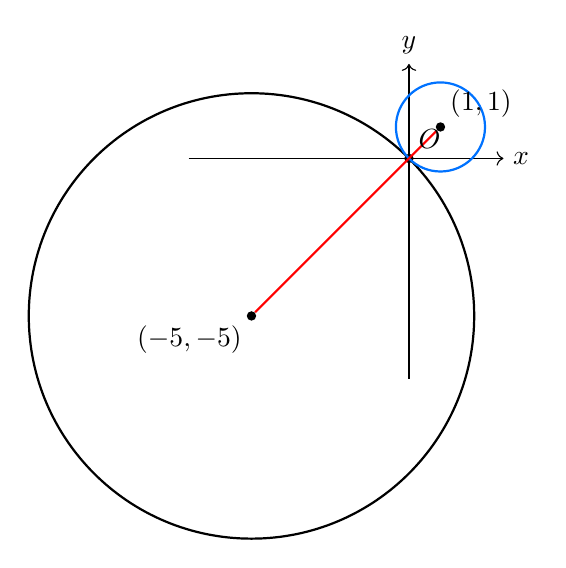
\begin{tikzpicture}[scale=0.4,baseline=(current bounding box.north)]
		\draw[->](-7,0)--(3,0) node[right]{$x$};
		\draw[->](0,-7)--(0,3) node[above]{$y$};
		\coordinate[circle,fill,inner sep=1.2pt] (Oa) at (-5,-5);
		\coordinate[circle,fill,inner sep=1.2pt] (Ob) at (1,1);
		\coordinate[circle,fill,inner sep=1.2pt] (O) at (0,0);
		\draw[thick] (Oa) circle({5*sqrt(2)});
		\draw[thick,SkyBlue] (Ob) circle({sqrt(2)});
		\draw[thick,red] (Oa)--(Ob);
		\node[below left] at (Oa) {$(-5,-5)$};
		\node[above right] at (Ob) {$(1,1)$};
		\node[above right] at (O) {$O$};
	\end{tikzpicture}
\end{minipage}

\begin{knowledge}{弦长公式}
	弦长$l=2\sqrt{r^2-d^2}$，其中$d$为圆心到直线的距离
\end{knowledge}

\category{弦长问题}
\begin{question}
	过$A(11,2)$作圆$x^2+y^2+2x-4y-164=0$的弦，弦长为整数的共有几个？
\end{question}

\begin{minipage}[t]{0.75\textwidth}
	圆方程配方：$(x+1)^2+(y-2)^2=169$，圆心$O(-1,2)$，半径$r=13$.
	
	点$A(11,2)$到圆心距离：$|OA|=\sqrt{(11+1)^2+(2-2)^2}=12<r$，故点在圆内.
	
	最短弦长（垂直于$OA$）：$l_{\min}=2\sqrt{13^2-12^2}=2\sqrt{25}=10$
	
	最长弦长（直径）：$l_{\max}=2r=26$
	
	弦长取值范围：$[10,26]$，整数弦长有$10,11,12,\cdots,26$共$17$个值.
	
	\begin{enumerate}[label=\arabic*.]
		\item 弦长为$10$（最短弦）：只有$1$条
		\item 弦长为$26$（直径）：只有$1$条
		\item 弦长为$11,12,\cdots,25$：共$15$个值，由圆的对称性，每个值对应$2$条弦
	\end{enumerate}
	
	合计：$1+1+15\times2=32$条.
\end{minipage}
\hfill
\begin{minipage}[t]{0.3\textwidth}
	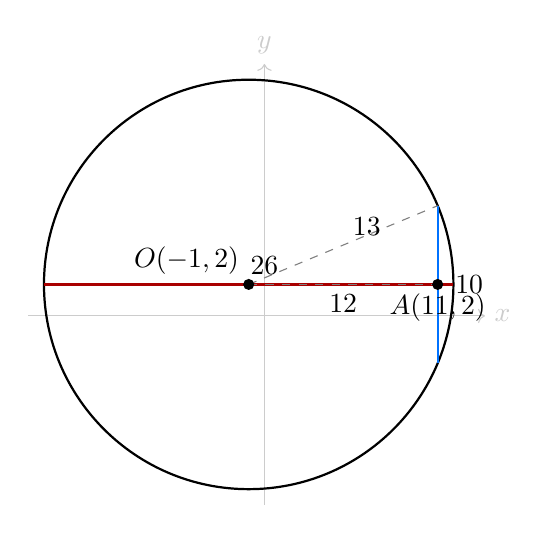
\begin{tikzpicture}[scale=0.2,baseline=(current bounding box.north)]
		\coordinate (O) at (-1,2);
		\coordinate (A) at (11,2);
		\coordinate (shortTop) at (11,7);
		\coordinate (shortBot) at (11,-3);
		\coordinate (longLeft) at (-14,2);
		\coordinate (longRight) at (12,2);
		
		% 坐标轴
		\draw[->,gray!40] (-15,0) -- (14,0) node[right] {$x$};
		\draw[->,gray!40] (0,-12) -- (0,16) node[above] {$y$};
		
		% 圆
		\draw[thick] (O) circle (13);
		
		% 最长弦（直径，红色）
		\draw[thick,DarkRed] (longLeft) -- (longRight);
		
		% 最短弦（蓝色，垂直于OA）
		\draw[thick,SkyBlue] (shortBot) -- (shortTop);
		
		% 辅助虚线：OA
		\draw[dashed,gray] (O) -- (A);
		
		% 辅助虚线：半径到最短弦端点
		\draw[dashed,gray] (O) -- (shortTop);
		
		% 标点
		\fill (O) circle (10pt) node[above left] {$O(-1,2)$};
		\fill (A) circle (10pt) node[below] {$A(11,2)$};
		
		% 标注
		\node[above] at (0,2) {$26$};
		\node[right] at (11.5,2) {$10$};
		\node[below] at (5,2) {$12$};
		\node[above right] at (5,4.5) {$13$};
	\end{tikzpicture}
\end{minipage}

\subsection{第五讲\quad 椭圆初步}

\subsubsection{椭圆的定义}
\begin{knowledge}{椭圆的定义}
	与两定点$F_1,F_2$的距离的和为常数（大于$|F_1F_2|$）的轨迹叫椭圆.
	\[
	\begin{aligned}
		|MF_1|+|MF_2| &> |F_1F_2|=2c \quad \text{椭圆} \\
		|MF_1|+|MF_2| &= |F_1F_2|=2c \quad \text{线段} \\
		|MF_1|+|MF_2| &< |F_1F_2|=2c \quad \text{不存在}
	\end{aligned}
	\]
\end{knowledge}

\category{代数求方程}
\begin{question}
	已知椭圆$\dfrac{x^2}{a^2}+\dfrac{y^2}{b^2}=1$的焦点为$(3,0)$，且$a=2b$，求椭圆的方程.
\end{question}
\begin{enumerate}[label=\arabic*.]
	\item 焦点位置：$x$轴
	\item 两个条件：$\begin{cases} a=2b \\ a^2=b^2+c^2 \end{cases}$，焦点$(3,0)\implies c=3$
\end{enumerate}
$\therefore a=2\sqrt{3},\ b=\sqrt{3},\ c=3$，椭圆方程：$\dfrac{x^2}{12}+\dfrac{y^2}{3}=1$.

\subsubsection{椭圆的标准方程}
\begin{knowledge}{标准方程}
	\[
	\frac{x^2}{a^2}+\frac{y^2}{b^2}=1 \qquad a^2=b^2+c^2
	\]
	\textbf{判断焦点位置：}谁的分母大，焦点在谁那，谁就是$a^2$.
\end{knowledge}

\category{代数求方程}
\begin{question}
	椭圆过定点$(3,0)$且$a=3b$，求标准方程.
\end{question}

过$(3,0)$并不是焦点，需分类讨论：
\begin{enumerate}[label=\arabic*.]
	\item 焦点在$x$轴：$\dfrac{x^2}{a^2}+\dfrac{y^2}{b^2}=1$.
	\newline $\because (3,0)$有个$0$，很特殊，代入$\dfrac{9}{a^2}=1\implies a=3,\ b=1$.
	\newline $\therefore \dfrac{x^2}{9}+y^2=1$.
	\item 焦点在$y$轴：$\dfrac{y^2}{a^2}+\dfrac{x^2}{b^2}=1$.
	\newline 将$(3,0)$代入$\dfrac{9}{b^2}=1\implies b=3,\ a=9$.
	\newline $\therefore \dfrac{y^2}{81}+\dfrac{x^2}{9}=1$.
\end{enumerate}

\subsubsection{几何性质}
\begin{knowledge}{几何性质}
	\begin{minipage}[t]{0.7\textwidth}
		\begin{itemize}
			\item 离心率：$e=\dfrac{c}{a}=\sqrt{1-\dfrac{b^2}{a^2}}=\sqrt{\dfrac{c^2}{b^2+c^2}}$等，平方再开根.
			\newline \textbf{性质：}$e$越大越扁.
			\item 通径：$|MN|=\dfrac{2b^2}{a}$（用$a^2=b^2+c^2$换值）.
		\end{itemize}
		
		\begin{knowledge}{求离心率的方法}
			\begin{enumerate}[label=\arabic*.]
				\item 找到$a,b,c$（初学）.
				\item 焦点三角形法（两焦点+一点在椭圆上）.
				\item 几何关系找到$a,b,c$等式.
			\end{enumerate}
		\end{knowledge}
		
		
		\begin{minipage}[t]{0.7\textwidth}
			\textbf{方法2举例：}
			
			在椭圆中，设$|PF_1|=7x, |PF_2|=3x$
			
			则$|F_1F_2|=2c=5x$.
			
			由椭圆定义：$|PF_1|+|PF_2|=2a=7x+3x=10x$.
			
			$\therefore e=\dfrac{c}{a}=\dfrac{5x}{10x}=\dfrac{1}{2}$.
		\end{minipage}
		\hfill
		\begin{minipage}[t]{0.2\textwidth}
			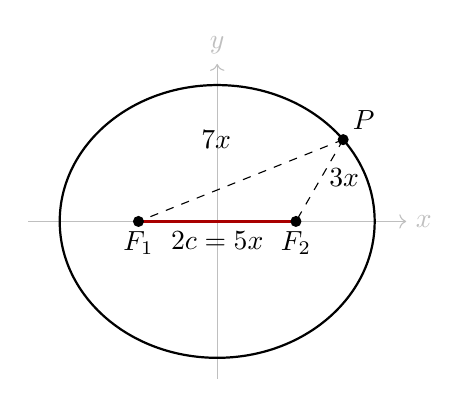
\begin{tikzpicture}[scale=0.2, baseline=(current bounding box.north)]
				\coordinate (F1) at (-5,0);
				\coordinate (F2) at (5,0);
				\coordinate (P) at (8, {sqrt(27)});
				\draw[->, gray!50] (-12,0) -- (12,0) node[right] {$x$};
				\draw[->, gray!50] (0,-10) -- (0,10) node[above] {$y$};
				\draw[thick] (0,0) ellipse (10 and {sqrt(75)});
				\draw[dashed] (P) -- (F1);
				\draw[dashed] (P) -- (F2);
				\draw[thick, DarkRed] (F1) -- (F2);
				\fill (F1) circle (10pt) node[below] {$F_1$};
				\fill (F2) circle (10pt) node[below] {$F_2$};
				\fill (P) circle (10pt) node[above right] {$P$};
				\node[below] at (0,0) {$2c=5x$};
				\node[above left] at (1.5,4) {$7x$};
				\node[below right] at (6.5,4) {$3x$};
			\end{tikzpicture}
		\end{minipage}
		
		\vspace{6pt}
		\textbf{方法3举例：}
		\begin{enumerate}[label=\arabic*.]
			\item 若$b=c$：
			\[
			e=\frac{c}{a}=\sqrt{\frac{c^2}{a^2}}=\sqrt{\frac{c^2}{b^2+c^2}}=\sqrt{\frac{1}{2}}=\frac{\sqrt{2}}{2}
			\]
			\item 若$b^2=ac$：
			\[
			a^2-c^2=ac \xrightarrow{\text{同除}a^2} 1-e^2=e
			\]
		\end{enumerate}
	\end{minipage}
	\hfill
	\begin{minipage}[t]{0.3\textwidth}
		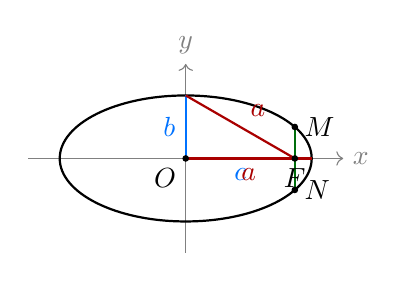
\begin{tikzpicture}[scale=0.8,baseline=(current bounding box.north)]
			\draw[->,gray] (-2.5,0) -- (2.5,0) node[right] {$x$};
			\draw[->,gray] (0,-1.5) -- (0,1.5) node[above] {$y$};
			\draw[thick] (0,0) ellipse (2 and 1);
			\coordinate (O) at (0,0);
			\coordinate (A) at (2,0);
			\coordinate (B) at (0,1);
			\coordinate (F) at ({sqrt(3)},0);
			\coordinate (M) at ({sqrt(3)},0.5);
			\coordinate (N) at ({sqrt(3)},-0.5);
			
			\draw[thick, SkyBlue] (O) -- (B) node[midway, left] {$b$};
			\draw[thick, SkyBlue] (O) -- (F) node[midway, below] {$c$};
			\draw[thick, DarkRed] (B) -- (F) node[midway, above right] {$a$};
			\draw[thick, DarkRed] (O) -- (A) node[midway, below] {$a$};
			\draw[thick, DarkGreen] (M) -- (N);
			
			\fill (O) circle (1.5pt) node[below left] {$O$};
			\fill (F) circle (1.5pt) node[below] {$F$};
			\fill (M) circle (1.5pt) node[right] {$M$};
			\fill (N) circle (1.5pt) node[right] {$N$};
		\end{tikzpicture}
	\end{minipage}
\end{knowledge}

\category{代数求方程}
\begin{question}
	过$(3,2)$且与椭圆$3x^2+8y^2=24$有相同焦点，求椭圆方程.
\end{question}

化简已知椭圆：$\dfrac{x^2}{8}+\dfrac{y^2}{3}=1$，焦点在$x$轴，$c^2=8-3=5$.

\textbf{A方法（待定系数法）：}
设椭圆方程为$\dfrac{x^2}{b^2+5}+\dfrac{y^2}{b^2}=1$.
代入$(3,2)$：
\[
\frac{9}{b^2+5}+\frac{4}{b^2}=1 \implies 9b^2+4(b^2+5)=b^2(b^2+5)
\]
\[
b^4-8b^2-20=0 \implies (b^2-10)(b^2+2)=0
\]
$\because b^2>0, \therefore b^2=10, a^2=15$.
方程为$\dfrac{x^2}{15}+\dfrac{y^2}{10}=1$.

\vspace{6pt}
\textbf{B方法（定义法）：}
\begin{minipage}[t]{0.65\textwidth}
	焦点$F_1(-\sqrt{5},0), F_2(\sqrt{5},0)$. 由定义 $|MF_1|+|MF_2|=2a$.
	\[
	2a = \sqrt{(3+\sqrt{5})^2+2^2} + \sqrt{(3-\sqrt{5})^2+2^2}
	\]
	\[
	2a = \sqrt{18+6\sqrt{5}} + \sqrt{18-6\sqrt{5}}
	\]
	两边平方：
	\[
	4a^2 = (18+6\sqrt{5}) + (18-6\sqrt{5}) + 2\sqrt{(18+6\sqrt{5})(18-6\sqrt{5})}
	\]
	\[
	4a^2 = 36 + 2\sqrt{324-180} = 36 + 24 = 60
	\]
	$\therefore a^2=15, b^2=a^2-c^2=10$.
	方程为$\dfrac{x^2}{15}+\dfrac{y^2}{10}=1$.
\end{minipage}
\hfill
\begin{minipage}[t]{0.35\textwidth}
	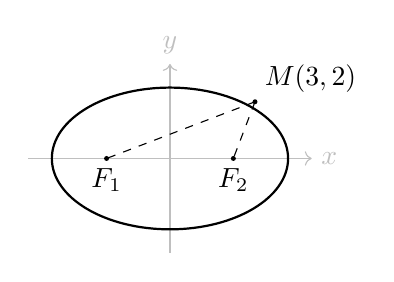
\begin{tikzpicture}[scale=0.6, baseline=(current bounding box.north)]
		\draw[->, gray!50] (-3,0) -- (3,0) node[right] {$x$};
		\draw[->, gray!50] (0,-2) -- (0,2) node[above] {$y$};
		\draw[thick] (0,0) ellipse (2.5 and 1.5);
		\coordinate (F1) at ({-sqrt(5)*0.6}, 0);
		\coordinate (F2) at ({sqrt(5)*0.6}, 0);
		\coordinate (M) at (1.8, 1.2);
		
		\draw[dashed] (M) -- (F1);
		\draw[dashed] (M) -- (F2);
		
		\fill (F1) circle (1.5pt) node[below] {$F_1$};
		\fill (F2) circle (1.5pt) node[below] {$F_2$};
		\fill (M) circle (1.5pt) node[above right] {$M(3,2)$};
	\end{tikzpicture}
\end{minipage}

\category{代数求方程}
\begin{question}
	椭圆$x^2+my^2=1$的焦点在$y$轴上，长轴是短轴的$2$倍，$m=$?
\end{question}

化为标准方程：$\dfrac{x^2}{1}+\dfrac{y^2}{1/m}=1$.

焦点在$y$轴，故$a^2=\dfrac{1}{m}, b^2=1$.

由$a=2b$：
\[
a=\sqrt{\frac{1}{m}}=2\times 1=2 \implies m=\frac{1}{4}.
\]

\category{离心率求方程}
\begin{question}
	椭圆离心率$e=\dfrac{\sqrt{3}}{2}$，过点$(2,1)$，$\dfrac{x^2}{a^2}+\dfrac{y^2}{b^2}=1\ (a>b>0)$，求方程.
\end{question}

\[
e=\frac{\sqrt{3}}{2}=\sqrt{\frac{a^2-b^2}{a^2}} \implies a^2=4b^2
\]
将$(2,1)$代入$\dfrac{x^2}{a^2}+\dfrac{y^2}{b^2}=1$：
\[
\frac{4}{4b^2}+\frac{1}{b^2}=1 \implies b^2=2,\ a^2=8.
\]
椭圆方程：$\dfrac{x^2}{8}+\dfrac{y^2}{2}=1$.

\category{几何求方程}
\begin{question}
	已知椭圆$\dfrac{x^2}{a^2}+\dfrac{y^2}{b^2}=1\ (a>b>0)$，$F_1,F_2$为焦点，$AB$在椭圆上，$AB\perp F_1F_2$于$F_2$，$|AB|=4$，$|F_1F_2|=2\sqrt{3}$，求方程.
\end{question}

\begin{minipage}[t]{0.7\textwidth}
	$|F_1F_2|=2c=2\sqrt{3} \implies c=\sqrt{3}$.
	
	$AB$为通径：$|AB|=\dfrac{2b^2}{a}=4 \implies b^2=2a$.
	
	又$b^2=a^2-c^2=a^2-3$，故：
	\[
	2a=a^2-3 \implies a^2-2a-3=0 \implies a=3.
	\]
	$\therefore b^2=6$.
	
	椭圆方程：$\dfrac{x^2}{9}+\dfrac{y^2}{6}=1$.
\end{minipage}
\hfill
\begin{minipage}[t]{0.3\textwidth}
	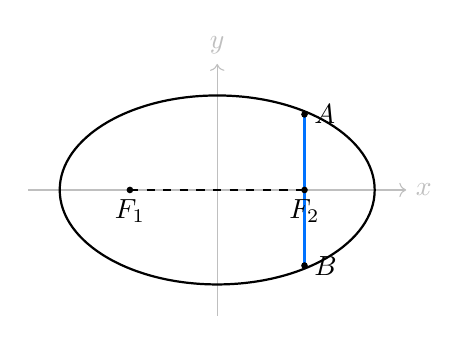
\begin{tikzpicture}[scale=0.8, baseline=(current bounding box.north)]
		\draw[->, gray!50] (-3,0) -- (3,0) node[right] {$x$};
		\draw[->, gray!50] (0,-2) -- (0,2) node[above] {$y$};
		\draw[thick] (0,0) ellipse (2.5 and 1.5);
		\coordinate (F1) at ({-sqrt(3)*0.8}, 0);
		\coordinate (F2) at ({sqrt(3)*0.8}, 0);
		\coordinate (A) at ({sqrt(3)*0.8}, 1.2);
		\coordinate (B) at ({sqrt(3)*0.8}, -1.2);
		
		\draw[thick, SkyBlue] (A) -- (B);
		\draw[dashed] (F1) -- (F2);
		
		\fill (F1) circle (1.5pt) node[below] {$F_1$};
		\fill (F2) circle (1.5pt) node[below] {$F_2$};
		\fill (A) circle (1.5pt) node[right] {$A$};
		\fill (B) circle (1.5pt) node[right] {$B$};
	\end{tikzpicture}
\end{minipage}

\category{找$a,b,c$求离心率}
\begin{question}
	已知椭圆$C:\dfrac{x^2}{a^2}+\dfrac{y^2}{4}=1\ (a>2)$，直线$l:y=x-2$过$C$的一个焦点，求$C$的离心率.
\end{question}

$\because a>2$

$\therefore$ 焦点在$x$轴上.

令$y=0$，得$x=2$，即焦点为$(2,0)$.

$\therefore c=2,\ b=2,\ a=\sqrt{b^2+c^2}=2\sqrt{2}$.

\[
e=\frac{c}{a}=\frac{2}{2\sqrt{2}}=\frac{\sqrt{2}}{2}.
\]

\category{焦点三角形法求离心率}
\begin{question}
	已知椭圆$\dfrac{x^2}{a^2}+\dfrac{y^2}{b^2}=1$左右焦点为$F_1,F_2$，$P$为椭圆上一点，且$\angle PF_1F_2=30^\circ$，$\angle PF_2F_1=60^\circ$，离心率=?
\end{question}

\begin{minipage}[t]{0.6\textwidth}
	在$\triangle PF_1F_2$中，$\angle F_1PF_2 = 180^\circ - 30^\circ - 60^\circ = 90^\circ$.
	
	设$|F_1F_2|=2c$.
	
	$|PF_2| = 2c \cdot \sin30^\circ = c$.
	
	$|PF_1| = 2c \cdot \cos30^\circ = \sqrt{3}c$.
	
	由定义 $|PF_1|+|PF_2|=2a$:
	
	$2a = \sqrt{3}c + c = (\sqrt{3}+1)c$.
	
	$\therefore e = \dfrac{2c}{2a} = \dfrac{2}{\sqrt{3}+1} = \sqrt{3}-1$.
\end{minipage}
\hfill
\begin{minipage}[t]{0.4\textwidth}
	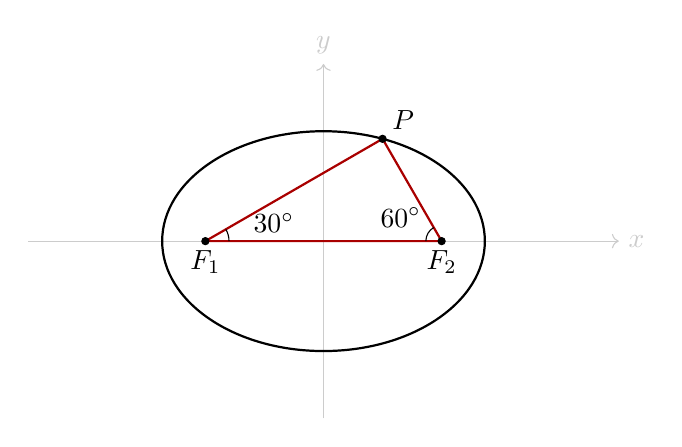
\begin{tikzpicture}[scale=1.5, baseline=(current bounding box.north)]
		\pgfmathsetmacro{\c}{1}
		\pgfmathsetmacro{\a}{(sqrt(3)+1)/2}
		\pgfmathsetmacro{\b}{sqrt(\a*\a - \c*\c)}
		
		\draw[->, gray!40] (-2.5,0) -- (2.5,0) node[right] {$x$};
		\draw[->, gray!40] (0,-1.5) -- (0,1.5) node[above] {$y$};
		
		\draw[thick] (0,0) ellipse (\a cm and \b cm);
		
		\coordinate (F1) at (-\c, 0);
		\coordinate (F2) at (\c, 0);
		\coordinate (P) at (0.5, {\c*sqrt(3)/2});
		
		\draw[thick, DarkRed] (F1) -- (P) -- (F2) -- cycle;
		
		\fill (F1) circle (1pt) node[below] {$F_1$};
		\fill (F2) circle (1pt) node[below] {$F_2$};
		\fill (P) circle (1pt) node[above right] {$P$};
		
		\draw pic["$30^\circ$", draw, angle eccentricity=3, angle radius=0.3cm] {angle = F2--F1--P};
		\draw pic["$60^\circ$", draw, angle eccentricity=3, angle radius=0.2cm] {angle = P--F2--F1};
	\end{tikzpicture}
\end{minipage}

\vspace{10pt}

\category{几何关系求离心率}
\begin{question}
	$PF_1$中点在$y$轴上，若$\angle PF_1F_2=30^\circ$，离心率=?
\end{question}

\begin{minipage}[t]{0.7\textwidth}
	设$PF_1$中点为$M$，$O$为原点（即$F_1F_2$中点）.
	
	$\therefore OM$为$\triangle PF_1F_2$的中位线
	
	$\therefore OM \parallel PF_2$.
	
	$\because M$在$y$轴上
	
	$\therefore OM \perp F_1F_2$（$x$轴）.
	
	$\therefore PF_2 \perp F_1F_2$，即$\triangle PF_1F_2$为直角三角形.
	
	设$|PF_2|=1$.
	
	$\because \angle PF_1F_2=30^\circ$
	
	$\therefore |PF_1|=2, |F_1F_2|=\sqrt{3}$.
	
	$2c = |F_1F_2| = \sqrt{3} \implies c=\dfrac{\sqrt{3}}{2}$.
	
	$2a = |PF_1|+|PF_2| = 2+1=3 \implies a=\dfrac{3}{2}$.
	
	$\therefore e = \dfrac{c}{a} = \dfrac{\frac{\sqrt{3}}{2}}{\frac{3}{2}} = \dfrac{\sqrt{3}}{3}$.
\end{minipage}
\hfill
\begin{minipage}[t]{0.3\textwidth}
	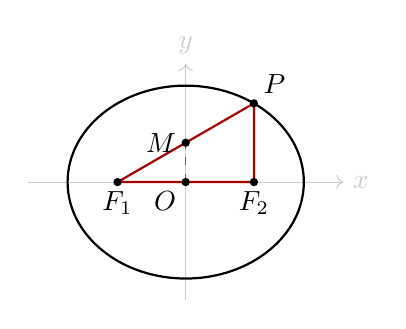
\begin{tikzpicture}[scale=0.5, baseline=(current bounding box.north)]
		\pgfmathsetmacro{\c}{sqrt(3)}
		\pgfmathsetmacro{\a}{3}
		\pgfmathsetmacro{\b}{sqrt(6)}
		
		\draw[->, gray!40] (-4,0) -- (4,0) node[right] {$x$};
		\draw[->, gray!40] (0,-3) -- (0,3) node[above] {$y$};
		
		\draw[thick] (0,0) ellipse (\a cm and \b cm);
		
		\coordinate (F1) at (-\c, 0);
		\coordinate (F2) at (\c, 0);
		\coordinate (O) at (0,0);
		\coordinate (P) at (\c, 2);
		\coordinate (M) at ($(F1)!0.5!(P)$);
		
		\draw[thick, DarkRed] (F1) -- (P) -- (F2) -- cycle;
		\draw[dashed, SkyBlue] (O) -- (M);
		
		\fill (F1) circle (3pt) node[below] {$F_1$};
		\fill (F2) circle (3pt) node[below] {$F_2$};
		\fill (O) circle (3pt) node[below left] {$O$};
		\fill (P) circle (3pt) node[above right] {$P$};
		\fill (M) circle (3pt) node[left] {$M$};
	\end{tikzpicture}
\end{minipage}

\subsection{第六讲\quad 双曲线初步}

\subsubsection{双曲线的定义}
\begin{knowledge}{双曲线的定义}
	与两定点$F_1,F_2$距离之差的绝对值等于常数(小于$|F_1F_2|$)的点的轨迹叫双曲线.
	\[
	\begin{aligned}
		||MF_1|-|MF_2|| &= 2a < |F_1F_2|=2c \quad \text{双曲线} \\
		||MF_1|-|MF_2|| &= 2a = |F_1F_2|=2c \quad \text{两条射线} \\
		||MF_1|-|MF_2|| &= 2a > |F_1F_2|=2c \quad \text{不存在}
	\end{aligned}
	\]
	不加绝对值为双曲线的一支(一条射线,不存在对应上).
	
	\textbf{注意：}$c$是老大.
\end{knowledge}

\category{焦点+点}
\begin{question}
	与双曲线$\dfrac{x^2}{16}-\dfrac{y^2}{4}=1$有相同焦点,且经过$(3\sqrt{2},2)$的双曲线标准方程?
\end{question}

$a^2=16, b^2=4, c^2=20=a^2+b^2$.

设所求方程为$\dfrac{x^2}{a^2}-\dfrac{y^2}{b^2}=1 \implies \dfrac{x^2}{20-b^2}-\dfrac{y^2}{b^2}=1$.

代入$(3\sqrt{2},2)$:
\[
\frac{18}{20-b^2}-\frac{4}{b^2}=1 \implies 18b^2-4(20-b^2)=b^2(20-b^2)
\]

通分整理：$b^4+2b^2-80=0 \implies (b^2+10)(b^2-8)=0$.

$\because b^2>0$

$\therefore b^2=8, a^2=12$.

$\therefore$ 方程为$\dfrac{x^2}{12}-\dfrac{y^2}{8}=1$.


\subsubsection{双曲线的标准方程}
\begin{knowledge}{标准方程}
	$\dfrac{x^2}{a^2}-\dfrac{y^2}{b^2}=1$ 或 $\dfrac{y^2}{a^2}-\dfrac{x^2}{b^2}=1$.
	谁的系数正,焦点在谁上($a^2$).
	
	一般式$mx^2+ny^2=1$:
	\begin{enumerate}[label=\arabic*.]
		\item $m=n>0$ 圆
		\item $m\neq n>0$ 椭圆
		\item $m\cdot n<0$ 双曲线
		\item $m<0,n<0$ 不存在
	\end{enumerate}
\end{knowledge}


\begin{question}
	若方程$\dfrac{x^2}{1+k}+\dfrac{y^2}{1-k}=1$表示双曲线,$k$范围?
\end{question}

$(1+k)(1-k)<0 \implies k \in (-\infty,-1)\cup(1,+\infty)$.

\category{点+渐近线}
\begin{question}
	已知双曲线过点$(1,\sqrt{2})$且渐近线为$y=\pm\sqrt{3}x$,方程?
\end{question}

\begin{minipage}[t]{0.7\textwidth}
	点+渐近线才可判断焦点位置.
	
	将$x=1$代入$y=\sqrt{3}x$中,$y=\sqrt{3}>\sqrt{2}$,过$x$轴.
	
	分析渐近线:$\sqrt{3}=\dfrac{b}{a}$.
	
	\textbf{A方法:} $\dfrac{x^2}{a^2}-\dfrac{y^2}{(\sqrt{3}a)^2}=1$
	
	代入$(1,\sqrt{2}) \implies a^2=\dfrac{1}{3}, b^2=1$.
	
	\textbf{B方法:} 共渐近线,写出$\sqrt{3}a=b$的方程:$x^2-\dfrac{y^2}{3}=\lambda$.
	
	代入$(1,\sqrt{2}) \implies \lambda=\dfrac{1}{3}$.
	
	$\therefore 3x^2-y^2=1$.
\end{minipage}
\hfill
\begin{minipage}[t]{0.3\textwidth}
	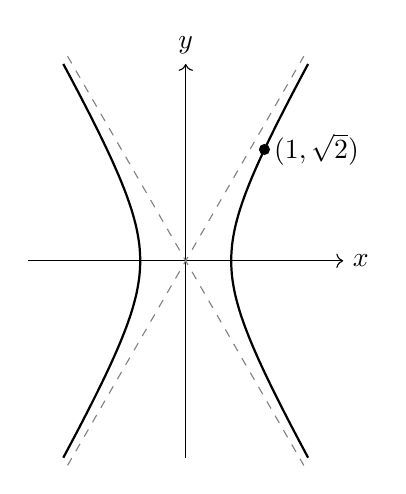
\begin{tikzpicture}[scale=1, baseline=(current bounding box.north)]
		\draw[->, black] (-2,0) -- (2,0) node[right] {$x$};
		\draw[->, black] (0,-2.5) -- (0,2.5) node[above] {$y$};
		
		\draw[thick, domain=-2.5:2.5, smooth, variable=\y] plot ({sqrt((\y*\y+1)/3)}, \y);
		\draw[thick, domain=-2.5:2.5, smooth, variable=\y] plot ({-sqrt((\y*\y+1)/3)}, \y);
		
		% 渐近线
		\draw[dashed, gray] (-1.5,{-1.5*sqrt(3)}) -- (1.5,{1.5*sqrt(3)});
		\draw[dashed, gray] (-1.5,{1.5*sqrt(3)}) -- (1.5,{-1.5*sqrt(3)});
		
		% 标点
		\fill (1,{sqrt(2)}) circle (2pt) node[right] {$(1,\sqrt{2})$};
	\end{tikzpicture}
\end{minipage}

\subsubsection{几何性质}
\begin{knowledge}{几何性质}
	\begin{minipage}[t]{0.7\textwidth}
		
		实轴为$2a$
		
		渐近线$y=\pm\dfrac{b}{a}x$(焦点在$x$轴)或$y=\pm\dfrac{a}{b}x$(焦点在$y$轴).
		
		类比斜率$\dfrac{y_F}{x_F}$.
	\end{minipage}
	\hfill
	\begin{minipage}[t]{0.3\textwidth}
	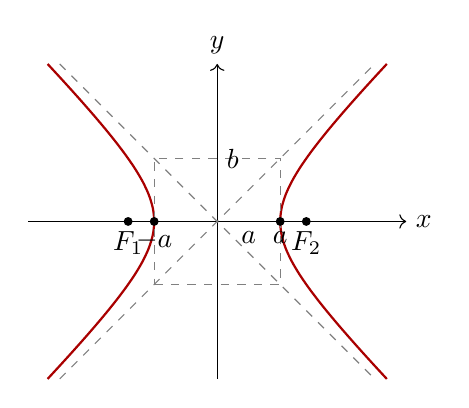
\begin{tikzpicture}[scale=0.8, baseline=(current bounding box.north)]
		% 坐标轴（黑色）
		\draw[->, black] (-3,0) -- (3,0) node[right] {$x$};
		\draw[->, black] (0,-2.5) -- (0,2.5) node[above] {$y$};
		
		% 双曲线
		\draw[thick, DarkRed, domain=-2.5:2.5, smooth, variable=\y] plot ({sqrt(1+\y*\y)}, \y);
		\draw[thick, DarkRed, domain=-2.5:2.5, smooth, variable=\y] plot ({-sqrt(1+\y*\y)}, \y);
		
		% 渐近线
		\draw[dashed, gray] (-2.5,-2.5) -- (2.5,2.5);
		\draw[dashed, gray] (-2.5,2.5) -- (2.5,-2.5);
		
		% 辅助矩形
		\draw[dashed, gray] (-1,-1) -- (1,-1) -- (1,1) -- (-1,1) -- cycle;
		
		% 坐标点
		\coordinate (F1) at (-{sqrt(2)},0);
		\coordinate (F2) at ({sqrt(2)},0);
		\coordinate (A1) at (-1,0);
		\coordinate (A2) at (1,0);
		
		% 标点
		\fill (F1) circle (2pt) node[below] {$F_1$};
		\fill (F2) circle (2pt) node[below] {$F_2$};
		\fill (A1) circle (2pt) node[below] {$-a$};
		\fill (A2) circle (2pt) node[below] {$a$};
		
		% 标注 a 和 b
		\node[right] at (0,1) {$b$};
		\node[below] at (0.5,0) {$a$};
	\end{tikzpicture}
	\end{minipage}
\end{knowledge}

\category{渐近线(多解)}
\begin{question}
	实轴为6,渐近线$y=\pm\dfrac{3}{2}x$的双曲线方程?
\end{question}

$2a=6, a=3$.
\begin{enumerate}[label=\arabic*.]
	\item 焦点在$x$轴:$\dfrac{b}{a}=\dfrac{3}{2} \implies a=3 \implies b=\dfrac{9}{2} \implies \dfrac{x^2}{9}-\dfrac{y^2}{\frac{81}{4}}=1$.
	\item 焦点在$y$轴:$\dfrac{a}{b}=\dfrac{3}{2} \implies a=3 \implies b=2 \implies \dfrac{y^2}{9}-\dfrac{x^2}{4}=1$.
\end{enumerate}

\category{焦点+共渐近线}
\begin{question}
	和椭圆$\dfrac{x^2}{49}+\dfrac{y^2}{24}=1$共焦点，和双曲线$\dfrac{x^2}{36}-\dfrac{y^2}{64}=1$共渐近线的双曲线方程？
\end{question}

椭圆中 $a^2=49, b^2=24 \implies c^2=25$，焦点在$x$轴.

双曲线渐近线斜率 $\dfrac{b}{a} = \sqrt{\dfrac{64}{36}} = \dfrac{4}{3}$.

设所求双曲线方程为 $\dfrac{x^2}{9\lambda} - \dfrac{y^2}{16\lambda} = 1\ (\lambda>0)$.

\[
c^2 = 9\lambda + 16\lambda = 25\lambda = 25 \implies \lambda=1.
\]
方程为 $\dfrac{x^2}{9} - \dfrac{y^2}{16} = 1$.

\category{通径}
\begin{question}
	过双曲线$\dfrac{x^2}{a^2}-\dfrac{y^2}{b^2}=1$的一个焦点作实轴的垂线，交双曲线于$A,B$两点，$|AB|=$实轴长，求离心率.
\end{question}

通径长 $|AB| = \dfrac{2b^2}{a}$.

由题意 $\dfrac{2b^2}{a} = 2a \implies a=b$.

\[
e = \frac{c}{a} = \sqrt{\frac{a^2+b^2}{a^2}} = \sqrt{2}.
\]

\category{焦点三角形}
\begin{question}
	焦点在$x$轴的双曲线，$P$为双曲线右支上一点，$\triangle OPF_2$为正三角形（$O$为原点，$F_2$为右焦点），求离心率.
\end{question}

\begin{minipage}[t]{0.7\textwidth}
	$\because \triangle OPF_2$ 为正三角形
	
	$\therefore |OP|=|OF_2|=|PF_2|=c$.
	
	在 $\triangle PF_1F_2$ 中，$|OP| = \dfrac{1}{2}|F_1F_2| = c$
	
	$\therefore \triangle PF_1F_2$ 为直角三角形，$\angle F_1PF_2 = 90^\circ$.
	
	\[
	|PF_2| = c, \quad |PF_1| = \sqrt{|F_1F_2|^2 - |PF_2|^2} = \sqrt{3}c.
	\]
	
	由定义 $|PF_1| - |PF_2| = 2a$:
	\[
	\sqrt{3}c - c = 2a \implies e = \frac{2c}{2a} = \frac{2}{\sqrt{3}-1} = \sqrt{3}+1.
	\]
\end{minipage}
\hfill
\begin{minipage}[t]{0.3\textwidth}
	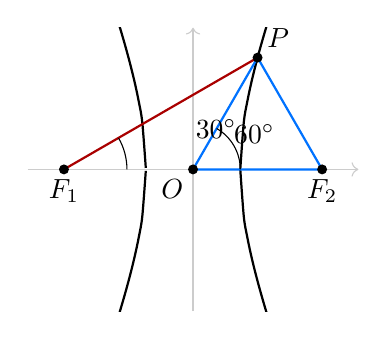
\begin{tikzpicture}[scale=0.6, baseline=(current bounding box.north)]
		\pgfmathsetmacro{\a}{1}
		\pgfmathsetmacro{\c}{sqrt(3)+1}
		\pgfmathsetmacro{\b}{sqrt(\c*\c - \a*\a)}
		\pgfmathsetmacro{\px}{\c/2}
		\pgfmathsetmacro{\py}{sqrt(3)*\c/2}
		
		% 先裁剪超出范围的部分
		\clip (-3.5,-3) rectangle (3.5,3);
		
		\draw[->, gray!40] (-3.5,0) -- (3.5,0) node[right] {$x$};
		\draw[->, gray!40] (0,-3) -- (0,3) node[above] {$y$};
		
		% 使用题目推导出的准确参数绘图，确保P在曲线上
		% 限制domain避免曲线太长
		\draw[thick, domain=1:2.8, smooth, variable=\x] plot ({\x}, {\b*sqrt(\x*\x-1)/\a});
		\draw[thick, domain=1:2.8, smooth, variable=\x] plot ({\x}, {-\b*sqrt(\x*\x-1)/\a});
		\draw[thick, domain=-2.8:-1, smooth, variable=\x] plot ({\x}, {\b*sqrt(\x*\x-1)/\a});
		\draw[thick, domain=-2.8:-1, smooth, variable=\x] plot ({\x}, {-\b*sqrt(\x*\x-1)/\a});
		
		\coordinate (F1) at (-\c, 0);
		\coordinate (F2) at (\c, 0);
		\coordinate (O) at (0,0);
		\coordinate (P) at (\px, \py);
		
		\draw[thick, SkyBlue] (O) -- (P) -- (F2) -- cycle;
		\draw[thick, DarkRed] (F1) -- (P);
		
		\fill (F1) circle (3pt) node[below] {$F_1$};
		\fill (F2) circle (3pt) node[below] {$F_2$};
		\fill (O) circle (3pt) node[below left] {$O$};
		\fill (P) circle (3pt) node[above right] {$P$};
		
		\draw pic["$30^\circ$", draw, angle eccentricity=2.5, angle radius=0.8cm] {angle = F2--F1--P};
		\draw pic["$60^\circ$", draw, angle eccentricity=1.5, angle radius=0.6cm] {angle = F2--O--P};
	\end{tikzpicture}
\end{minipage}

\category{几何关系}
\begin{question}
	焦点在$x$轴，直线$x=c$与双曲线渐近线交$A,B$，若$\triangle F_1AB$为等腰直角三角形（$F_1$为左焦点），求离心率.
\end{question}
\begin{minipage}[t]{0.7\textwidth}
	直线 $x=c$ 过右焦点 $F_2(c,0)$ 且垂直于 $x$ 轴.
	
	$A, B$ 在渐近线 $y=\pm\dfrac{b}{a}x$ 上
	
	$\therefore A(c, \dfrac{bc}{a}), B(c, -\dfrac{bc}{a})$.
	
	$\because \triangle F_1AB$ 为等腰直角三角形，且 $F_1F_2 \perp AB$
	
	$\therefore \angle AF_1F_2 = 45^\circ \implies |F_1F_2| = |AF_2|$.
	\[
	2c = \frac{bc}{a} \implies b=2a.
	\]
	\[
	e = \sqrt{1+\left(\frac{b}{a}\right)^2} = \sqrt{1+4} = \sqrt{5}.
	\]
\end{minipage}
\hfill
\begin{minipage}[t]{0.3\textwidth}
	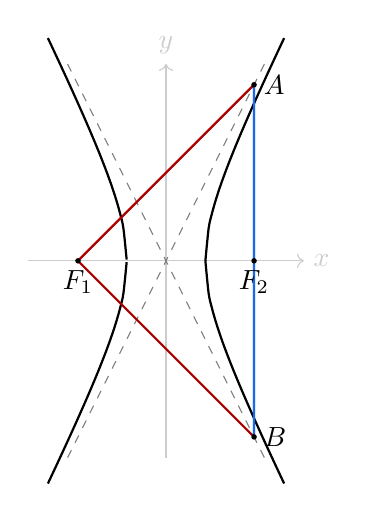
\begin{tikzpicture}[scale=0.5, baseline=(current bounding box.north)]
		\pgfmathsetmacro{\a}{1}
		\pgfmathsetmacro{\b}{2}
		\pgfmathsetmacro{\c}{sqrt(5)}
		
		% 坐标轴
		\draw[->, gray!40] (-3.5,0) -- (3.5,0) node[right] {$x$};
		\draw[->, gray!40] (0,-5) -- (0,5) node[above] {$y$};
		
		% 双曲线 x^2 - y^2/4 = 1
		\draw[thick, domain=1:3, smooth, variable=\x] plot ({\x}, {\b*sqrt(\x*\x-1)/\a});
		\draw[thick, domain=1:3, smooth, variable=\x] plot ({\x}, {-\b*sqrt(\x*\x-1)/\a});
		\draw[thick, domain=-3:-1, smooth, variable=\x] plot ({\x}, {\b*sqrt(\x*\x-1)/\a});
		\draw[thick, domain=-3:-1, smooth, variable=\x] plot ({\x}, {-\b*sqrt(\x*\x-1)/\a});
		
		% 渐近线 y = ±2x (斜率修正为 2)
		\draw[dashed, gray] (-2.5,-5) -- (2.5,5);
		\draw[dashed, gray] (-2.5,5) -- (2.5,-5);
		
		% 坐标点
		\coordinate (F1) at (-\c, 0);
		\coordinate (F2) at (\c, 0);
		% A, B 在渐近线上，x=c 时 y = ±(b/a)*c = ±2*sqrt(5)
		\coordinate (A) at (\c, {\b*\c/\a}); 
		\coordinate (B) at (\c, {-\b*\c/\a});
		
		% 连线
		\draw[thick, DarkRed] (F1) -- (A) -- (B) -- cycle;
		\draw[thick, SkyBlue] (A) -- (B);
		
		% 标点
		\fill (F1) circle (2pt) node[below] {$F_1$};
		\fill (F2) circle (2pt) node[below] {$F_2$};
		\fill (A) circle (2pt) node[right] {$A$};
		\fill (B) circle (2pt) node[right] {$B$};
	\end{tikzpicture}
\end{minipage}

\category{两次焦点三角形}
\begin{question}
	$P$在左支，$PF_2$和右支交点为$Q$，若$\triangle PF_1Q$为等边三角形，求离心率.
\end{question}

\begin{minipage}[t]{0.7\textwidth}
	两个焦点三角形：$\triangle PF_1F_2, \triangle QF_1F_2$.
	
	$\triangle PF_1F_2$: $PF_2 - PF_1 = 2a$.
	
	$\because \triangle PF_1Q$ 为等边三角形
	
	$\therefore PF_1 = F_1Q = PQ = x$.
	
	又 $P, Q, F_2$ 共线
	
	$\therefore PF_2 = PQ + QF_2 = x + QF_2$.
	
	$\therefore QF_2 = PF_2 - PF_1 = 2a$.
	
	$\triangle QF_1F_2$: $QF_1 - QF_2 = 2a$.
	
	$\therefore x - 2a = 2a \implies x = 4a$.
	
	在 $\triangle PF_1F_2$ 中，$\angle F_1PF_2 = 60^\circ$.
	
	由余弦定理：
	\[
	F_1F_2^2 = PF_1^2 + PF_2^2 - 2PF_1 \cdot PF_2 \cdot \cos 60^\circ
	\]
	\[
	4c^2 = (4a)^2 + (6a)^2 - 2(4a)(6a) \cdot \frac{1}{2} = 28a^2
	\]
	
	$\therefore c = \sqrt{7}a, e = \sqrt{7}$.
\end{minipage}
\hfill
\begin{minipage}[t]{0.3\textwidth}
	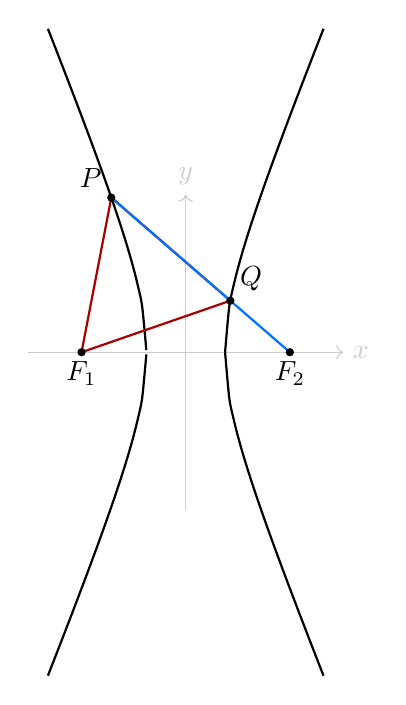
\begin{tikzpicture}[scale=0.5, baseline=(current bounding box.north)]
		\pgfmathsetmacro{\a}{1}
		\pgfmathsetmacro{\c}{sqrt(7)}
		\pgfmathsetmacro{\b}{sqrt(6)}
		
		\draw[->, gray!40] (-4,0) -- (4,0) node[right] {$x$};
		\draw[->, gray!40] (0,-4) -- (0,4) node[above] {$y$};
		
		% 双曲线 x^2 - y^2/6 = 1
		\draw[thick, domain=1:3.5, smooth, variable=\x] plot ({\x}, {\b*sqrt(\x*\x-1)/\a});
		\draw[thick, domain=1:3.5, smooth, variable=\x] plot ({\x}, {-\b*sqrt(\x*\x-1)/\a});
		\draw[thick, domain=-3.5:-1, smooth, variable=\x] plot ({\x}, {\b*sqrt(\x*\x-1)/\a});
		\draw[thick, domain=-3.5:-1, smooth, variable=\x] plot ({\x}, {-\b*sqrt(\x*\x-1)/\a});
		
		\coordinate (F1) at (-\c, 0);
		\coordinate (F2) at (\c, 0);
		\coordinate (P) at ({-5/\c}, {sqrt(108/7)});
		\coordinate (Q) at ({3/\c}, {sqrt(12/7)});
		
		\draw[thick, DarkRed] (P) -- (F1) -- (Q) -- cycle;
		\draw[thick, SkyBlue] (P) -- (F2);
		
		\fill (F1) circle (3pt) node[below] {$F_1$};
		\fill (F2) circle (3pt) node[below] {$F_2$};
		\fill (P) circle (3pt) node[above left] {$P$};
		\fill (Q) circle (3pt) node[above right] {$Q$};
	\end{tikzpicture}
\end{minipage}

\subsection{第七讲\quad 抛物线初步}

\subsubsection{定义}
\begin{knowledge}{抛物线的定义}
	平面内与一个定点 $F$ 和一条定直线 $l$ ($l$ 不经过 $F$) 的距离相等的点的轨迹叫抛物线.
	\begin{itemize}
		\item 定点 $F$：焦点.
		\item 定直线 $l$：准线.
		\item $F$ 与 $l$ 的距离为焦准距 $p$ ($p>0$).
	\end{itemize}
	\textbf{注意：}若 $F$ 在 $l$ 上，轨迹为过 $F$ 且垂直于 $l$ 的直线.
\end{knowledge}

\category{圆锥曲线定义对比}
\begin{enumerate}[label=\arabic*.]
	\item 一个定点：圆（到定点距离为定值）.
	\item 两个定点（对称）：
	\begin{itemize}
		\item 椭圆：$|PF_1|+|PF_2|=2a$ ($2a > |F_1F_2|$)
		\item 双曲线：$||PF_1|-|PF_2||=2a$ ($2a < |F_1F_2|$)
	\end{itemize}
	\item 一个直线 + 一个点：直线或抛物线.
\end{enumerate}

\subsubsection{标准方程}
\begin{knowledge}{标准方程形式}
	$y^2=2px$ ($p>0$).
	\begin{itemize}
		\item \textbf{判断焦点位置：}谁是一次项，焦点在谁上（$x$ 或 $y$ 轴）.
		\item \textbf{判断开口方向：}系数正，开口向正半轴；系数负，开口向负半轴.
		\item \textbf{焦点坐标：}一次项变量轴上，坐标值为 $\frac{1}{4} \times$ 一次项系数（即 $\frac{p}{2}$）.
	\end{itemize}
\end{knowledge}

\begin{question}
	已知抛物线 $y=\frac{1}{2}x^2$，求准线方程.
\end{question}

化为标准方程：$x^2=2y$.
焦点在 $y$ 轴，$2p=2 \implies p=1$.
焦点 $(0, \frac{1}{2})$，准线 $y=-\frac{1}{2}$.

\begin{question}
	求过点 $(1,2)$ 的抛物线方程.
\end{question}

\begin{minipage}[t]{0.7\textwidth}
	需分类讨论开口方向：
	\begin{enumerate}[label=\arabic*.]
		\item 开口向上（焦点在 $y$ 轴）：设 $x^2=2py$.
		代入 $(1,2) \implies 1=4p \implies 2p=\frac{1}{2}$.
		方程：$x^2=\frac{1}{2}y$.
		\item 开口向右（焦点在 $x$ 轴）：设 $y^2=2px$.
		代入 $(1,2) \implies 4=2p$.
		方程：$y^2=4x$.
	\end{enumerate}
\end{minipage}
\hfill
\begin{minipage}[t]{0.3\textwidth}
	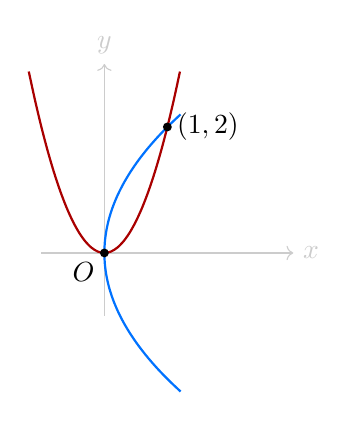
\begin{tikzpicture}[scale=0.8, baseline=(current bounding box.north)]
		\draw[->, gray!40] (-1,0) -- (3,0) node[right] {$x$};
		\draw[->, gray!40] (0,-1) -- (0,3) node[above] {$y$};
		% x^2 = 0.5y => y = 2x^2
		\draw[thick, DarkRed, domain=-1.2:1.2, smooth, variable=\x] plot ({\x}, {2*\x*\x});
		% y^2 = 4x => x = 0.25y^2
		\draw[thick, SkyBlue, domain=-2.2:2.2, smooth, variable=\y] plot ({0.25*\y*\y}, {\y});
		
		\fill (1,2) circle (2pt) node[right] {$(1,2)$};
		\fill (0,0) circle (2pt) node[below left] {$O$};
	\end{tikzpicture}
\end{minipage}

\subsubsection{定义与焦准距转化}
\begin{question}
	若焦准距为 2，求抛物线方程.
\end{question}

$p=2$.抛物线有四种开口方向：
\[
\begin{cases}
	x^2 = \pm 2py = \pm 4y \\
	y^2 = \pm 2px = \pm 4x
\end{cases}
\]

\begin{knowledge}{焦半径公式（定义转化）}
	设 $P(x_0, y_0)$ 为抛物线 $y^2=2px$ 上一点.
	
	$|PF| = |P\text{到准线}| = x_0 + \frac{p}{2}$.
	
	\textbf{用途：}涉及抛物线上一点到焦点的距离，常转化为到准线的距离.
\end{knowledge}

\begin{minipage}[t]{0.7\textwidth}
	
	
	\textbf{示例：}
	对于 $y^2=2px$，准线 $x=-\frac{p}{2}$.
	
	$|PF| = x_0 - (-\frac{p}{2}) = x_0 + \frac{p}{2}$.
	
	对于 $x^2=2py$，准线 $y=-\frac{p}{2}$.
	$|PF| = y_0 - (-\frac{p}{2}) = y_0 + \frac{p}{2}$.
\end{minipage}
\hfill
\begin{minipage}[t]{0.3\textwidth}
	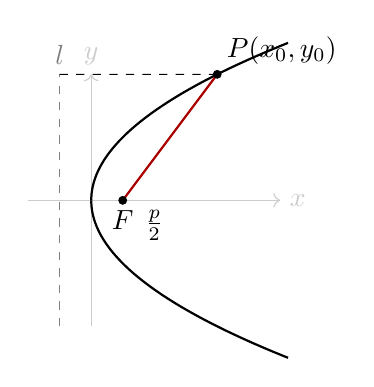
\begin{tikzpicture}[scale=0.8, baseline=(current bounding box.north)]
		\draw[->, gray!40] (-1,0) -- (3,0) node[right] {$x$};
		\draw[->, gray!40] (0,-2) -- (0,2) node[above] {$y$};
		% y^2 = 2x (p=1)
		\draw[thick, domain=0:2.5, smooth, variable=\y] plot ({0.5*\y*\y}, {\y});
		\draw[thick, domain=0:2.5, smooth, variable=\y] plot ({0.5*\y*\y}, {-\y});
		
		\coordinate (F) at (0.5, 0);
		\coordinate (P) at (2, 2); % 2^2 = 2*2 no, 4=4. y^2=2x -> 4=2*2. P(2,2) is on y^2=2x? 4=4 yes.
		% Wait, y^2=2px. If p=1, y^2=2x. P(2,2) -> 4=4. Correct.
		% Focus (0.5, 0). Directrix x = -0.5.
		
		\draw[dashed, gray] (-0.5,-2) -- (-0.5,2) node[above] {$l$};
		\draw[dashed] (P) -- (-0.5, 2); % Perpendicular to directrix
		\draw[thick, DarkRed] (P) -- (F);
		
		\fill (F) circle (2pt) node[below] {$F$};
		\fill (P) circle (2pt) node[above right] {$P(x_0,y_0)$};
		\node[below] at (1, 0) {$\frac{p}{2}$};
	\end{tikzpicture}
\end{minipage}

\subsubsection{将军饮马问题}
	\begin{minipage}{0.5\textwidth}
		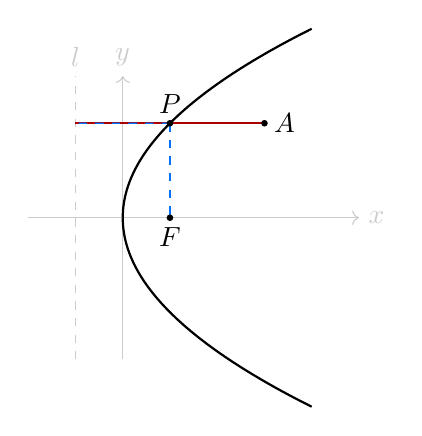
\begin{tikzpicture}[scale=0.6, baseline=(current bounding box.north)]
			\draw[->, gray!40] (-2,0) -- (5,0) node[right] {$x$};
			\draw[->, gray!40] (0,-3) -- (0,3) node[above] {$y$};
			\draw[dashed, gray!40] (-1,-3) -- (-1,3) node[above] {$l$};
			
			% 抛物线 y^2=4x
			\draw[thick, domain=0:4, smooth, variable=\y] plot ({0.25*\y*\y}, {\y});
			\draw[thick, domain=0:4, smooth, variable=\y] plot ({0.25*\y*\y}, {-\y});
			
			\coordinate (F) at (1,0);
			\coordinate (A) at (3,2);
			\coordinate (P) at (1,2);
			\coordinate (Aproj) at (-1,2);
			
			% 最短路径：A到准线的垂线
			\draw[thick, DarkRed] (A) -- (Aproj);
			% 转化：|PF| = d
			\draw[dashed, SkyBlue] (P) -- (F);
			\draw[dashed, SkyBlue] (P) -- (-1,2);
			
			\fill[black] (F) circle (2pt) node[below] {$F$};
			\fill[black] (A) circle (2pt) node[right] {$A$};
			\fill[black] (P) circle (2pt) node[above] {$P$};
		\end{tikzpicture}
		
		$AP+PF=x_A+\dfrac{p}{2}$
	\end{minipage}
	\hfill
	\begin{minipage}{0.5\textwidth}
		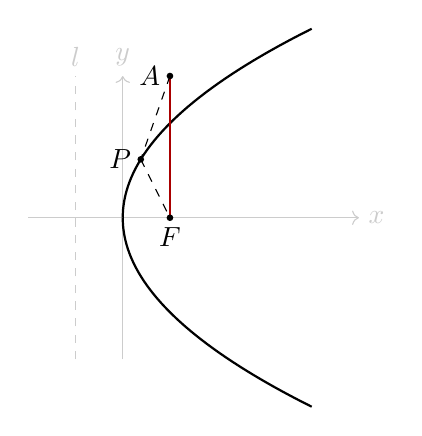
\begin{tikzpicture}[scale=0.6, baseline=(current bounding box.north)]
			\draw[->, gray!40] (-2,0) -- (5,0) node[right] {$x$};
			\draw[->, gray!40] (0,-3) -- (0,3) node[above] {$y$};
			\draw[dashed, gray!40] (-1,-3) -- (-1,3) node[above] {$l$};
			
			% 抛物线 y^2=4x
			\draw[thick, domain=0:4, smooth, variable=\y] plot ({0.25*\y*\y}, {\y});
			\draw[thick, domain=0:4, smooth, variable=\y] plot ({0.25*\y*\y}, {-\y});
			
			\pgfmathsetmacro{\px}{(3-sqrt(5))/2}
			\pgfmathsetmacro{\py}{sqrt(5)-1}
			
			\coordinate (F) at (1,0);
			\coordinate (A) at (1,3);
			\coordinate (P) at (\px, \py);
			
			% 最短路径：|AF|
			\draw[thick, DarkRed] (A) -- (F);
			% 转化：d = |PF|
%			\draw[dashed, SkyBlue] (P) -- (-1, \py);
%			\draw[dashed, SkyBlue] (P) -- (F);
			
			\fill[black] (F) circle (2pt) node[below] {$F$};
			\fill[black] (A) circle (2pt) node[left] {$A$};
			\fill[black] (P) circle (2pt) node[left] {$P$};
			\draw[dashed,black] (A)--(P);
			\draw[dashed,black] (P)--(F);
		\end{tikzpicture}
		
		$(AP+PF)_\text{min}=AF$
	\end{minipage}

\category{将军饮马问题（定义转化）}
\begin{question}
	已知抛物线$y^2=2px$经过点$M(x_0, 2\sqrt{2})$，若$M$到准线$l$距离为$3$，求方程.
\end{question}

$M$到$l$距离$= x_0 + \dfrac{p}{2} = 3$.

将$M$代入抛物线方程：$(2\sqrt{2})^2 = 2px_0 \implies 8 = 2px_0 \implies x_0 = \dfrac{4}{p}$.

$\dfrac{p}{2} + \dfrac{4}{p} = 3 \implies p^2 - 6p + 8 = 0 \implies p=4$或$p=2$.

$\therefore$方程为$y^2=4x$或$y^2=8x$.

\subsubsection{相似三角形问题}
\begin{knowledge}{梯形中位线推广}
	如图，直角梯形上底为$a$，下底为$b$.
	
	若中间平行线$c$将腰分为$1:3$（上段:下段），则：
	\[
	c = \frac{3}{4}a + \frac{1}{4}b
	\]
	\textbf{应用：}在抛物线焦点弦问题中，若$\overrightarrow{AF}=\lambda\overrightarrow{FB}$，则焦准距$p$满足定比分点关系.
\end{knowledge}

\begin{minipage}[t]{0.7\textwidth}
	\textbf{推导：}
	设上底$a$，下底$b$，高$h$.
	腰被分为$1:3$，则$c$距离上底$\frac{1}{4}h$.
	由相似三角形或线性插值：
	\[
	c = a + \frac{1}{4}(b-a) = \frac{3}{4}a + \frac{1}{4}b
	\]
\end{minipage}
\hfill
\begin{minipage}[t]{0.3\textwidth}
	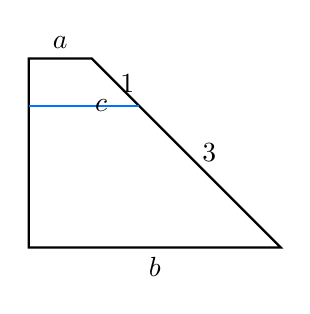
\begin{tikzpicture}[scale=0.8, baseline=(current bounding box.north)]
		\coordinate (A) at (0, 3);
		\coordinate (B) at (1, 3);
		\coordinate (C) at (4, 0);
		\coordinate (D) at (0, 0);
		\coordinate (P) at (1.75, 2.25);
		\coordinate (Q) at (0, 2.25);
		
		\draw[thick] (D) -- (C) -- (B) -- (A) -- cycle;
		\draw[thick, SkyBlue] (Q) -- (P);
		
		\node[above] at (0.5, 3) {$a$};
		\node[below] at (2, 0) {$b$};
		\node[right] at (0.9, 2.25) {$c$};
		
		\node[right] at (1.3, 2.6) {$1$};
		\node[right] at (2.6, 1.5) {$3$};
	\end{tikzpicture}
\end{minipage}

\category{相似三角形问题（最值）}
\begin{question}
	已知$y^2=4x$，$A(5,3)$，$M$为抛物线上一点，求$\triangle MAF$周长最小值.
\end{question}

\begin{minipage}[t]{0.7\textwidth}
	$F(1,0)$，准线$l: x=-1$.
	
	$|AF| = \sqrt{(5-1)^2 + 3^2} = 5$（定值）.
	
	周长$C = |MA| + |MF| + |AF| = |MA| + d(M, l) + 5$.
	
	当$M, A$与$M$在准线上的投影$M'$三点共线（即$MA \perp l$）时，
	
	$|MA| + d(M, l)$最小.
	
	最小值$= d(A, l) = 5 - (-1) = 6$.
	
	$\therefore C_{\min} = 6 + 5 = 11$.
\end{minipage}
\hfill
\begin{minipage}[t]{0.3\textwidth}
	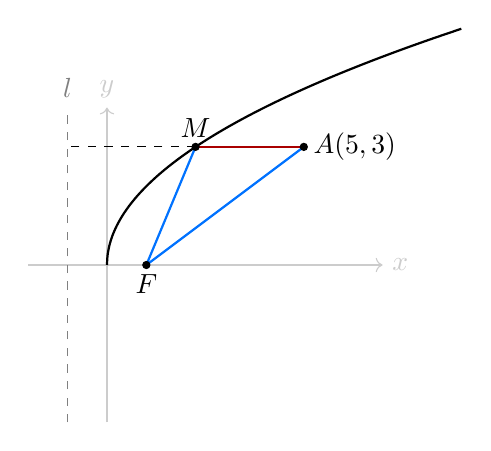
\begin{tikzpicture}[scale=0.5, baseline=(current bounding box.north)]
		\draw[->, gray!40] (-2,0) -- (7,0) node[right] {$x$};
		\draw[->, gray!40] (0,-4) -- (0,4) node[above] {$y$};
		\draw[dashed, gray] (-1,-4) -- (-1,4) node[above] {$l$};
		% y^2=4x
		\draw[thick, domain=0:6, smooth, variable=\y] plot ({0.25*\y*\y}, {\y});
		
		\coordinate (F) at (1,0);
		\coordinate (A) at (5,3);
		\coordinate (M) at (2.25, 3); % y=3, x=9/4=2.25
		
		\draw[thick, DarkRed] (A) -- (M);
		\draw[thick, SkyBlue] (M) -- (F);
		\draw[thick, SkyBlue] (A) -- (F);
		\draw[dashed] (M) -- (-1, 3);
		
		\fill (F) circle (3pt) node[below] {$F$};
		\fill (A) circle (3pt) node[right] {$A(5,3)$};
		\fill (M) circle (3pt) node[above] {$M$};
	\end{tikzpicture}
\end{minipage}

\begin{question}
	$P$在抛物线$y^2=4x$上，则$P$到$A(0,-1)$的距离与到直线$x=-1$的距离之和的最小值.
\end{question}

\begin{minipage}[t]{0.7\textwidth}
	$P$到直线$x=-1$（准线）的距离等于$|PF|$（$F$为焦点$(1,0)$）.
	
	即求$|PA| + |PF|$的最小值.
	
	$\because$ 线段$AF$与抛物线相交.
	
	$\therefore$ 最小值$= |AF| = \sqrt{(1-0)^2 + (0-(-1))^2} = \sqrt{2}$.
\end{minipage}
\hfill
\begin{minipage}[t]{0.3\textwidth}
	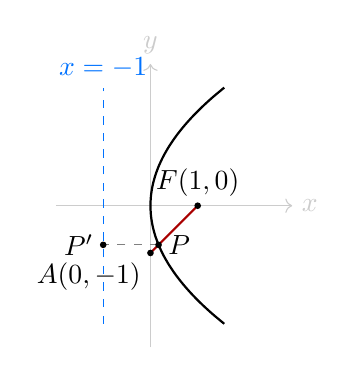
\begin{tikzpicture}[scale=0.6, baseline=(current bounding box.north)]
		\draw[->, gray!40] (-2,0) -- (3,0) node[right] {$x$};
		\draw[->, gray!40] (0,-3) -- (0,3) node[above] {$y$};
		
		% 抛物线 y^2=4x
		\draw[thick, domain=-2.5:2.5, smooth, variable=\y] plot ({0.25*\y*\y}, {\y});
		
		% 准线 x=-1
		\draw[dashed, SkyBlue] (-1,-2.5) -- (-1,2.5) node[above] {$x=-1$};
		
		% 坐标点
		\coordinate (A) at (0,-1);
		\coordinate (F) at (1,0);
		\coordinate (P) at ({3-2*sqrt(2)}, {2-2*sqrt(2)});
		\coordinate (P_proj) at (-1, {2-2*sqrt(2)});
		
		% 连线
		\draw[thick, DarkRed] (A) -- (F);
		\draw[dashed, gray] (P) -- (P_proj);
		
		% 标点
		\fill (A) circle (2pt) node[below left] {$A(0,-1)$};
		\fill (F) circle (2pt) node[above] {$F(1,0)$};
		\fill (P) circle (2pt) node[right] {$P$};
		\fill (P_proj) circle (2pt) node[left] {$P'$};
	\end{tikzpicture}
\end{minipage}

\category{焦点弦与向量}
\begin{question}
	已知$y^2=4x$，$A,B$在抛物线上，$\overrightarrow{AF}=3\overrightarrow{FB}$，则$|AB|=$?
\end{question}

\begin{minipage}[t]{0.7\textwidth}
	$p=2$，焦点$F(1,0)$，准线$x=-1$.
	
	设$|BF|=x$，则$|AF|=3x$，$|AB|=4x$.
	
	由梯形中位线推广（或相似三角形）：
	$F$到准线距离$p=2$.
	
	$A, B$到准线距离分别为$|AF|=3x, |BF|=x$.
	
	$F$分$AB$为$3:1$，则$p = \dfrac{1 \cdot |AF| + 3 \cdot |BF|}{1+3}$（定比分点公式）.
	
	$2 = \dfrac{3x + 3x}{4} = \dfrac{6x}{4} = \dfrac{3}{2}x$.
	
	$\therefore x = \dfrac{4}{3}$.
	
	$\therefore |AB| = 4x = \dfrac{16}{3}$.
\end{minipage}
\hfill
\begin{minipage}[t]{0.3\textwidth}
	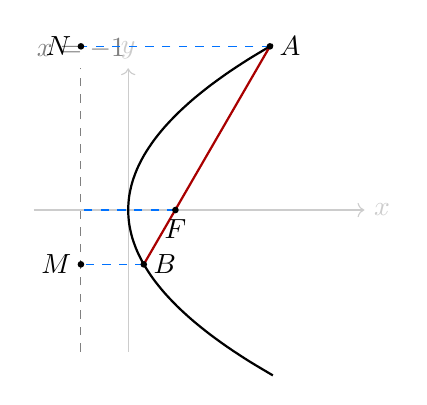
\begin{tikzpicture}[scale=0.6, baseline=(current bounding box.north)]
		\draw[->, gray!40] (-2,0) -- (5,0) node[right] {$x$};
		\draw[->, gray!40] (0,-3) -- (0,3) node[above] {$y$};
		\draw[dashed, gray] (-1,-3) -- (-1,3) node[above] {$x=-1$};
		% y^2=4x
		\draw[thick, domain=-3.5:3.5, smooth, variable=\y] plot ({0.25*\y*\y}, {\y});
		
		\coordinate (F) at (1,0);
		\coordinate (A) at (3, {2*sqrt(3)}); % approx (3, 3.46)
		\coordinate (B) at (0.33, {-1.15}); % approx (1/3, -2sqrt(3)/3)
		\coordinate (N) at (-1, {2*sqrt(3)});
		\coordinate (M) at (-1, {-1.15});
		
		\draw[thick, DarkRed] (A) -- (B);
		\draw[dashed, SkyBlue] (A) -- (N);
		\draw[dashed, SkyBlue] (B) -- (M);
		\draw[dashed, SkyBlue] (F) -- (-1, 0);
		
		\fill (F) circle (2pt) node[below] {$F$};
		\fill (A) circle (2pt) node[right] {$A$};
		\fill (B) circle (2pt) node[right] {$B$};
		\fill (N) circle (2pt) node[left] {$N$};
		\fill (M) circle (2pt) node[left] {$M$};
	\end{tikzpicture}
\end{minipage}

\subsection{第八讲\quad 轨迹方程}

\subsubsection{圆锥曲线综合(求方程/离心率)}

\begin{knowledge}{}
	求方程：
	
	双曲线/椭圆：焦点+ 2条件
	
	抛物线：焦点位置$\Bigg\{(\pm \dfrac{p}{2},0) ~\text{or}~ (0,\pm \dfrac{p}{2})\Bigg\}$+ 1条件 求p
\end{knowledge}


\category{圆锥曲线综合}
\begin{question}
	双曲线$C_1:\dfrac{x^2}{a^2}-\dfrac{y^2}{b^2}=1\ (e=2)$，抛物线$C_2:x^2=2py\ (p>0)$的焦点到双曲线$C_1$的渐近线的距离为$2$，求抛物线方程.
\end{question}

抛物线焦点坐标为$(0, \dfrac{p}{2})$.

由双曲线离心率$e=\sqrt{1+\dfrac{b^2}{a^2}}=2 \implies \dfrac{b}{a}=\sqrt{3}$.

渐近线方程为$y=\pm\sqrt{3}x \implies \sqrt{3}x-y=0$.

由点到直线距离公式：
\[
d = \frac{|\sqrt{3}\cdot 0 - \frac{p}{2}|}{\sqrt{(\sqrt{3})^2+(-1)^2}} = \dfrac{\frac{p}{2}}{2} = 2 \implies p=8.
\]

$\therefore$ 抛物线方程为$x^2=16y$.

\category{轨迹方程（面积法）}
\begin{question}
	已知椭圆$\dfrac{x^2}{a^2}+\dfrac{y^2}{b^2}=1$的$e=\dfrac{\sqrt{2}}{2}$，双曲线$x^2-y^2=1$的渐近线与椭圆有$4$个交点，$4$交点围成的四边形$S=16$，求椭圆方程.
\end{question}

\begin{minipage}[t]{0.7\textwidth}
	双曲线$x^2-y^2=1$的渐近线为$y=\pm x$（倾斜角$45^\circ$）.
	
	由椭圆离心率$e=\dfrac{c}{a}=\dfrac{\sqrt{2}}{2} \implies a^2=2b^2$.
	
	渐近线$y=\pm x$与坐标轴夹角$45^\circ$，围成的四边形为正方形（对角线在$y=\pm x$上）.
	
	$\because S=16$，由对称性，第一象限交点为$(2,2)$.
	
	将$a^2=2b^2$及点$(2,2)$代入椭圆方程：
	\[
	\frac{4}{2b^2} + \frac{4}{b^2} = 1 \implies \frac{2}{b^2} + \frac{4}{b^2} = 1 \implies b^2=6.
	\]
	$\therefore a^2=12$.
	
	椭圆方程为$\dfrac{x^2}{12}+\dfrac{y^2}{6}=1$.
\end{minipage}
\hfill
\begin{minipage}[t]{0.3\textwidth}
	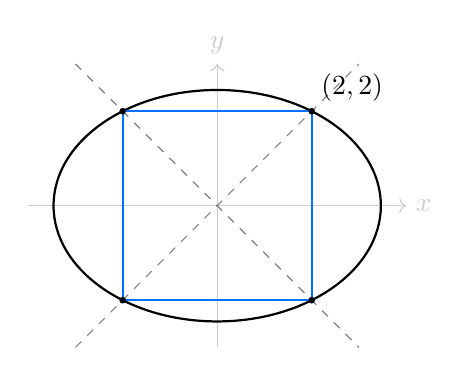
\begin{tikzpicture}[scale=0.6, baseline=(current bounding box.north)]
		\draw[->, gray!40] (-4,0) -- (4,0) node[right] {$x$};
		\draw[->, gray!40] (0,-3) -- (0,3) node[above] {$y$};
		
		% 椭圆 x^2/12 + y^2/6 = 1 -> a=sqrt(12)~3.46, b=sqrt(6)~2.45
		\draw[thick] (0,0) ellipse ({sqrt(12)} and {sqrt(6)});
		
		% 渐近线 y=x, y=-x
		\draw[dashed, gray] (-3,-3) -- (3,3);
		\draw[dashed, gray] (-3,3) -- (3,-3);
		
		% 交点 (2,2), (-2,2), (-2,-2), (2,-2)
		\coordinate (P1) at (2,2);
		\coordinate (P2) at (-2,2);
		\coordinate (P3) at (-2,-2);
		\coordinate (P4) at (2,-2);
		
		\draw[thick, SkyBlue] (P1) -- (P2) -- (P3) -- (P4) -- cycle;
		
		\fill (P1) circle (2pt) node[above right] {$(2,2)$};
		\fill (P2) circle (2pt);
		\fill (P3) circle (2pt);
		\fill (P4) circle (2pt);
	\end{tikzpicture}
\end{minipage}

\category{共焦点问题}
\begin{question}
	如图，$F_1,F_2$为椭圆$\dfrac{x^2}{4}+y^2=1$与双曲线的共焦点. 若$AF_1BF_2$为矩形，求双曲线的离心率.
\end{question}

\begin{minipage}[t]{0.7\textwidth}
	椭圆中$a_1^2=4, b_1^2=1 \implies c^2=3 \implies c=\sqrt{3}$.
	
	双曲线与椭圆共焦点，故双曲线$c=\sqrt{3}$.
	
	$\because$ 四边形$AF_1BF_2$为矩形
	
	$\therefore$ 对角线相等且互相平分.
	
	$\therefore |OA|=|OF_1|=c$.
	
	$\therefore \triangle F_1AF_2$为直角三角形，$\angle F_1AF_2=90^\circ$.
	
	由椭圆定义：$|AF_1|+|AF_2|=2a_1=4$.
	
	由勾股定理：$|AF_1|^2+|AF_2|^2=|F_1F_2|^2=(2c)^2=12$.
	
	联立解得：$2|AF_1||AF_2| = (|AF_1|+|AF_2|)^2 - (|AF_1|^2+|AF_2|^2) = 16-12=4$.
	
	由双曲线定义：$2a_2 = ||AF_2|-|AF_1||$.
	
	$(2a_2)^2 = (|AF_2|-|AF_1|)^2 = |AF_1|^2+|AF_2|^2 - 2|AF_1||AF_2| = 12-4=8$.
	
	$\therefore 4a_2^2=8 \implies a_2=\sqrt{2}$.
	
	$\therefore$ 双曲线离心率$e_2 = \dfrac{c}{a_2} = \dfrac{\sqrt{3}}{\sqrt{2}} = \dfrac{\sqrt{6}}{2}$.
\end{minipage}
\hfill
\begin{minipage}[t]{0.3\textwidth}
	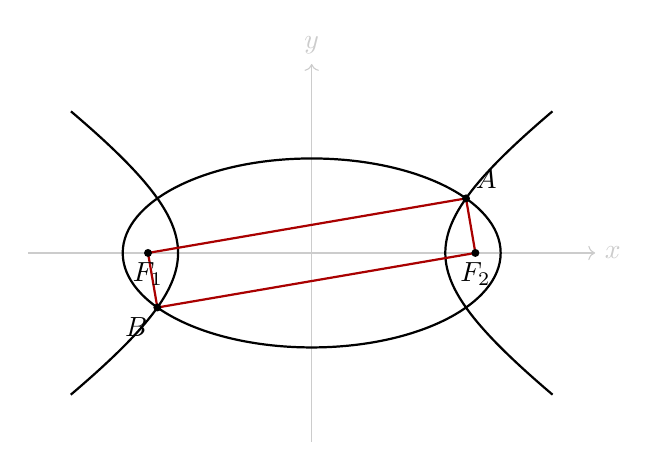
\begin{tikzpicture}[scale=1.2, baseline=(current bounding box.north)]
		\draw[->, gray!40] (-3,0) -- (3,0) node[right] {$x$};
		\draw[->, gray!40] (0,-2) -- (0,2) node[above] {$y$};
		
		% 椭圆 x^2/4 + y^2 = 1
		\draw[thick] (0,0) ellipse (2 and 1);
		
		% 双曲线 x^2/2 - y^2 = 1，使用y作自变量避免断点和负数开方
		\draw[thick, domain=-1.5:1.5, smooth, samples=100, variable=\y] plot ({sqrt(2*(\y*\y+1))}, {\y});
		\draw[thick, domain=-1.5:1.5, smooth, samples=100, variable=\y] plot ({-sqrt(2*(\y*\y+1))}, {\y});
		
		\coordinate (F1) at ({-sqrt(3)}, 0);
		\coordinate (F2) at ({sqrt(3)}, 0);
		\coordinate (A) at ({sqrt(8/3)}, {sqrt(1/3)});
		\coordinate (B) at ({-sqrt(8/3)}, {-sqrt(1/3)});
		
		\draw[thick, DarkRed] (A) -- (F1) -- (B) -- (F2) -- cycle;
		
		\fill (F1) circle (1.2pt) node[below] {$F_1$};
		\fill (F2) circle (1.2pt) node[below] {$F_2$};
		\fill (A) circle (1.2pt) node[above right] {$A$};
		\fill (B) circle (1.2pt) node[below left] {$B$};
	\end{tikzpicture}
\end{minipage}

\subsection*{2. 轨迹方程}

\begin{knowledge}{直接法}
	翻动条件形成数字表达式.
	
	注意分母不为0，$\triangle ABC$ (不共线).
\end{knowledge}

\begin{question}
	自圆 $(x-3)^2+(y+4)^2=4$ 外一点 $P(x,y)$ 引一条切线，切线长 $=OP$，求 $P$ 的轨迹方程.
\end{question}

\begin{minipage}[t]{0.7\textwidth}
	圆心 $C(3,-4)$，半径 $r=2$.
	
	切线长 $PQ = \sqrt{PC^2-r^2} = \sqrt{(x-3)^2+(y+4)^2-4}$.
	
	$OP = \sqrt{x^2+y^2}$.
	
	由题意 $PQ=OP \implies PQ^2=OP^2$.
	
	$(x-3)^2+(y+4)^2-4 = x^2+y^2$.
	
	$x^2-6x+9+y^2+8y+16-4 = x^2+y^2$.
	
	$-6x+8y+21=0$.
	
	$\therefore 6x-8y-21=0$.
\end{minipage}
\hfill
\begin{minipage}[t]{0.3\textwidth}
	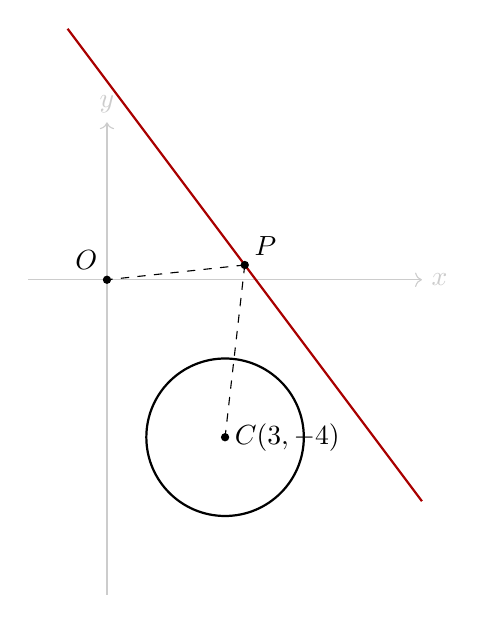
\begin{tikzpicture}[scale=0.5, baseline=(current bounding box.north)]
		\draw[->, gray!40] (-2,0) -- (8,0) node[right] {$x$};
		\draw[->, gray!40] (0,-8) -- (0,4) node[above] {$y$};
		
		\coordinate (C) at (3,-4);
		\coordinate (O) at (0,0);
		\coordinate (P) at (3.5, 0.375); % 6(3.5)-8(0.375)-21 = 21-3-21=-3 approx 0
		
		\draw[thick] (C) circle (2);
		\draw[thick, DarkRed] (-1, 6.375) -- (8, -5.625); % 6x-8y-21=0 -> y = 0.75x - 2.625
		
		\draw[dashed] (P) -- (C);
		\draw[dashed] (P) -- (O);
		
		\fill (C) circle (3pt) node[right] {$C(3,-4)$};
		\fill (O) circle (3pt) node[above left] {$O$};
		\fill (P) circle (3pt) node[above right] {$P$};
	\end{tikzpicture}
\end{minipage}

\category{定义法}
\begin{knowledge}{曲线类型判断}
	根据 $mx^2+ny^2=1$:
	\begin{enumerate}
		\item $m=n>0$ 圆.
		
		\item $m \neq n > 0$ 椭圆.
		
		\item $m \cdot n < 0$ 双曲线.
		
		\item $m, n < 0$ 不存在.
	\end{enumerate}
	
	\textbf{猜哪种曲线步骤：}
	\begin{enumerate}
		\item 一点：圆.
		
		\item 两点：椭圆 ($|PF_1|+|PF_2|=2a, a>c$)，双曲线 ($||PF_1|-|PF_2||=2a, c>a$) $\implies$ 双曲线一支 (有范围).
		
		\item 一点一线：抛物线.
	\end{enumerate}
\end{knowledge}



\category{相关点法}
\begin{knowledge}{相关点法步骤}
	\begin{enumerate}
		\item 设轨迹点 $(x,y)$，相关点 $(x_0,y_0)$.
		
		\item 用 $x,y$ 表示 $x_0,y_0$.
		
		\item 分离 $x_0,y_0$.
		
		\item 把 $x_0,y_0$ 代入相关表达式中.
	\end{enumerate}
\end{knowledge}

\begin{question}
	$P$ 是 $x^2+y^2+4x-12y+39=0$ 上的动点，直线 $x-y+1=0$ 是 $PQ$ 中垂线，求 $Q$ 的轨迹方程.
\end{question}

\begin{minipage}[t]{0.7\textwidth}
	圆方程：$(x+2)^2+(y-6)^2=1$，圆心 $C(-2,6)$，半径 $r=1$.
	
	设 $Q(x,y), P(x_0,y_0)$.
	
	$PQ \perp l$ 且中点在 $l$ 上.
	
	$\begin{cases} \frac{y-y_0}{x-x_0} = -1 \\ \frac{x_0+x}{2} - \frac{y_0+y}{2} + 1 = 0 \end{cases} \implies \begin{cases} x_0 = y-1 \\ y_0 = x+1 \end{cases}$
	
	代入圆方程 $(x_0+2)^2+(y_0-6)^2=1$:
	
	$(y-1+2)^2 + (x+1-6)^2 = 1$.
	
	$\therefore (x-5)^2 + (y+1)^2 = 1$.
\end{minipage}
\hfill
\begin{minipage}[t]{0.3\textwidth}
	\begin{tikzpicture}[scale=0.5, baseline=(current bounding box.north)]
		\draw[->, gray!40] (-6,0) -- (6,0) node[right] {$x$};
		\draw[->, gray!40] (0,-4) -- (0,10) node[above] {$y$};
		
		\coordinate (C) at (-2,6);
		\coordinate (P) at (-1.5, 6.866); % on circle
		\coordinate (Q) at (5.866, 0.5); % symmetric to P wrt x-y+1=0
		
		\draw[thick] (C) circle (1);
		\draw[thick, DarkRed] (-4, -3) -- (6, 7); % x-y+1=0 -> y=x+1
		\draw[dashed] (P) -- (Q);
		\draw[dashed, SkyBlue] (C) -- (P);
		
		\fill (C) circle (3pt) node[left] {$C$};
		\fill (P) circle (3pt) node[above] {$P$};
		\fill (Q) circle (3pt) node[right] {$Q$};
	\end{tikzpicture}
\end{minipage}

\begin{question}
	有一圆，圆心为 $O$，$Q$ 为圆外一点，$A$ 为圆上一点，使圆折叠后 $A$ 与 $Q$ 重合，折痕 $CD$ 与 $OA$ 交于 $P$，求 $P$ 的轨迹是什么图形.
\end{question}

\begin{minipage}[t]{0.7\textwidth}
	折叠 $\implies PA=PQ$.
	
	$P$ 在 $OA$ 直线上.
	
	$|PO - PQ| = |PO - PA| = OA = r$ (半径).
	
	$O, Q$ 是定点，$r$ 是常数.
	
	$\because Q$ 在圆外
	
	$\therefore OQ > r$.
	
	$\therefore |PO - PQ| = r < OQ$.
	
	$\therefore$ 轨迹为双曲线.
\end{minipage}
\hfill
\begin{minipage}[t]{0.3\textwidth}
	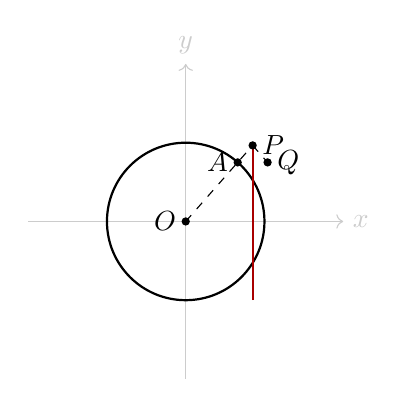
\begin{tikzpicture}[scale=0.5, baseline=(current bounding box.north)]
		\draw[->, gray!40] (-4,0) -- (4,0) node[right] {$x$};
		\draw[->, gray!40] (0,-4) -- (0,4) node[above] {$y$};
		
		\coordinate (O) at (0,0);
		\coordinate (Q) at (2.08,1.5);
		\coordinate (A) at (1.32, 1.5); % on circle r=2
		\coordinate (P) at (1.7, 1.931818); % on OA
		
		\draw[thick] (O) circle (2);
		\draw[thick, DarkRed] (1.7, -2) -- (1.7, 2); % Perpendicular bisector of AQ approx
		\draw[dashed] (O) -- (P);
		\draw[dashed] (P) -- (Q);
		
		\fill (O) circle (3pt) node[left] {$O$};
		\fill (Q) circle (3pt) node[right] {$Q$};
		\fill (A) circle (3pt) node[left] {$A$};
		\fill (P) circle (3pt) node[right] {$P$};
	\end{tikzpicture}
\end{minipage}

\category{动圆轨迹问题（定义法）}
\begin{question}
	动圆$M$与定圆$(x+2)^2+y^2=4$外切，且与直线$x=2$相切，求$M$的轨迹.
\end{question}

\begin{minipage}[t]{0.7\textwidth}
	定圆圆心$C(-2,0)$，半径$r=2$.
	
	设动圆$M$半径为$R$.
	由外切：$|MC| = R+2$.
	由与直线$x=2$相切：$M$到直线$x=2$的距离$d=R$.
	
	$\therefore \sqrt{(x+2)^2+y^2}-2=2-x$
	
	$\therefore y^2 = -12(x-1)$，即$y^2+12x-12=0$.
\end{minipage}
\hfill
\begin{minipage}[t]{0.3\textwidth}
	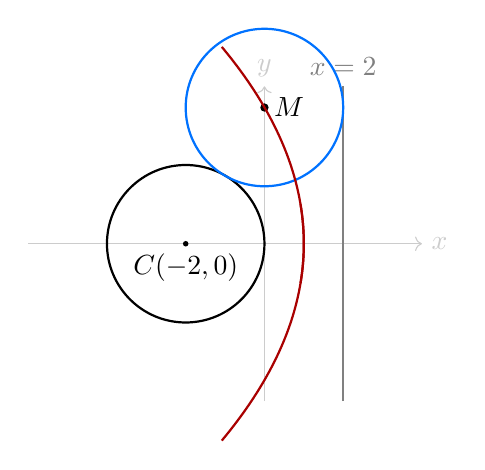
\begin{tikzpicture}[scale=0.5, baseline=(current bounding box.north)]
		\draw[->, gray!40] (-6,0) -- (4,0) node[right] {$x$};
		\draw[->, gray!40] (0,-4) -- (0,4) node[above] {$y$};
		
		% 定圆
		\draw[thick] (-2,0) circle (2);
		\fill (-2,0) circle (2pt) node[below] {$C(-2,0)$};
		
		% 直线 x=2
		\draw[thick, gray] (2,-4) -- (2,4) node[above] {$x=2$};
		
		% 动圆 M (示意)
		\coordinate (M) at (0, 2.45); % y^2 = -12(0-1) -> y=sqrt(12)~3.46. 取x=0, y=3.46. R=2.
		% 修正：取x=0, y^2=12, y=2sqrt(3)~3.46. R=2.
		% 距离C: sqrt(2^2 + 12) = 4. R+2 = 2+2=4. 对.
		\coordinate (M) at (0, 3.46);
		\draw[thick, SkyBlue] (M) circle (2);
		\fill (M) circle (3pt) node[right] {$M$};
		
		% 轨迹抛物线 y^2 = -12(x-1)
		\draw[thick, DarkRed, domain=-5:1, smooth, variable=\y] plot ({1-\y*\y/12}, {\y});
		\draw[thick, DarkRed, domain=-5:1, smooth, variable=\y] plot ({1-\y*\y/12}, {-\y});
		
	\end{tikzpicture}
\end{minipage}

\begin{question}
	动圆$P$与定圆$B:x^2+y^2+4x=0$相切，且过点$A(2,0)$，求$P$的轨迹.
\end{question}

\begin{minipage}{0.7\textwidth}
定圆$B$：$(x+2)^2+y^2=4$，圆心$B(-2,0)$，半径$R=2$.

动圆$P$过点$A(2,0)$，设半径为$r$，则$|PA|=r$.

\textbf{情况1：外切}

$|PB| = R+r = 2+r$.

$|PB| - |PA| = 2$.

\textbf{情况2：内切}

$|PB| = |r-R| = |r-2|$.

若$P$包围$B$，则$r>2$，$|PB|=r-2$.

$|PA| - |PB| = r - (r-2) = 2$.


综上：$||PA|-|PB|| = 2$.

$\because |AB|=4 > 2$

$\therefore$ 轨迹为双曲线.

$2a=2 \implies a=1$. $2c=4 \implies c=2$.

$b^2 = c^2-a^2 = 3$.

方程：$x^2 - \dfrac{y^2}{3} = 1$.
\end{minipage}
\hfill
\begin{minipage}{0.3\textwidth}
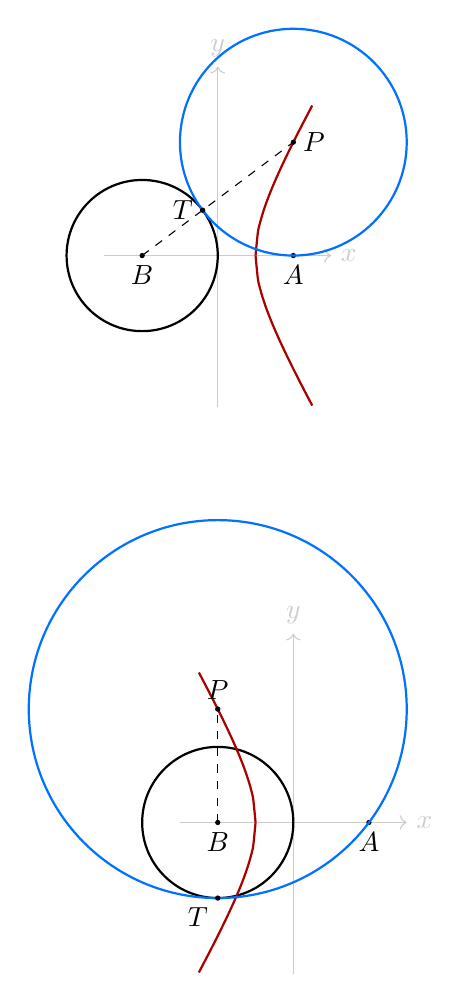
\begin{tikzpicture}[scale=0.48, baseline=(current bounding box.north)]
	% 左图：外切 (对应双曲线右支)
	\begin{scope}[shift={(-2,5)}]
		\draw[->, gray!40] (-3,0) -- (3,0) node[right] {$x$};
		\draw[->, gray!40] (0,-4) -- (0,5) node[above] {$y$};
		
		% 定圆 B
		\draw[thick] (-2,0) circle (2);
		\fill (-2,0) circle (2pt) node[below] {$B$};
		\fill (2,0) circle (2pt) node[below] {$A$};
		
		% 双曲线右支
		\draw[thick, DarkRed, domain=1:2.5, smooth, variable=\x] plot ({\x}, {sqrt(3*(\x*\x-1))});
		\draw[thick, DarkRed, domain=1:2.5, smooth, variable=\x] plot ({\x}, {-sqrt(3*(\x*\x-1))});
		
		% 动圆 P (圆心(2,3), 半径3)
		\coordinate (P) at (2,3);
		\draw[thick, SkyBlue] (P) circle (3);
		\fill (P) circle (2pt) node[right] {$P$};
		
		% 辅助线与切点 T(-0.4, 1.2)
		\draw[dashed] (-2,0) -- (2,3);
		\fill (-0.4, 1.2) circle (2pt) node[left] {$T$};
	\end{scope}
	
	% 右图：内切 (对应双曲线左支)
	\begin{scope}[shift={(0,-10)}]
		\draw[->, gray!40] (-3,0) -- (3,0) node[right] {$x$};
		\draw[->, gray!40] (0,-4) -- (0,5) node[above] {$y$};
		
		% 定圆 B
		\draw[thick] (-2,0) circle (2);
		\fill (-2,0) circle (2pt) node[below] {$B$};
		\fill (2,0) circle (2pt) node[below] {$A$};
		
		% 双曲线左支
		\draw[thick, DarkRed, domain=-2.5:-1, smooth, variable=\x] plot ({\x}, {sqrt(3*(\x*\x-1))});
		\draw[thick, DarkRed, domain=-2.5:-1, smooth, variable=\x] plot ({\x}, {-sqrt(3*(\x*\x-1))});
		
		% 动圆 P (圆心(-2,3), 半径5)
		\coordinate (P) at (-2,3);
		\draw[thick, SkyBlue] (P) circle (5);
		\fill (P) circle (2pt) node[above] {$P$};
		
		% 辅助线与切点 T(-2, -2)
		\draw[dashed] (-2,0) -- (-2,3);
		\fill (-2,-2) circle (2pt) node[below left] {$T$};
	\end{scope}
\end{tikzpicture}
\end{minipage}

\category{根式方程求轨迹}
\begin{question}
	$M(x,y)$在运动时，满足$\sqrt{9+x^2+y^2+6y} - \sqrt{9+x^2-6y+y^2} = 4$，求$M$轨迹.
\end{question}

\begin{minipage}[t]{0.7\textwidth}
	化简根式：
	\[
	\sqrt{x^2+(y+3)^2} - \sqrt{x^2+(y-3)^2} = 4
	\]
	几何意义：$M$到点$F_1(0,-3)$的距离减去$M$到点$F_2(0,3)$的距离等于$4$.
	\[
	|MF_1| - |MF_2| = 4 = 2a
	\]
	$\because 2a=4 < |F_1F_2|=6$
	
	$\therefore$ 轨迹为双曲线的一支.
	
	焦点在$y$轴，$c=3, a=2$.
	
	$b^2 = c^2-a^2 = 9-4=5$.
	
	$\because |MF_1| > |MF_2|$，$M$离$F_2(0,3)$更近.
	
	$\therefore$ 轨迹为双曲线的上支.
	
	方程：$\dfrac{y^2}{4} - \dfrac{x^2}{5} = 1 \quad (y \ge 2)$.
\end{minipage}
\hfill
\begin{minipage}[t]{0.3\textwidth}
	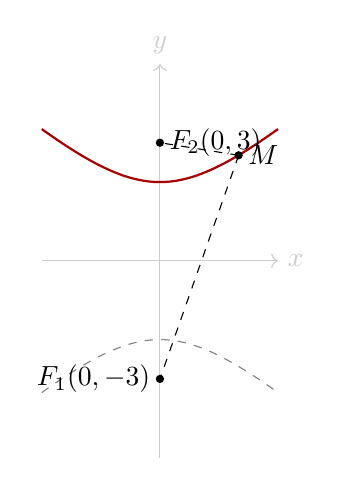
\begin{tikzpicture}[scale=0.5, baseline=(current bounding box.north)]
		\draw[->, gray!40] (-3,0) -- (3,0) node[right] {$x$};
		\draw[->, gray!40] (0,-5) -- (0,5) node[above] {$y$};
		
		% 双曲线 y^2/4 - x^2/5 = 1
		% y = 2*sqrt(1 + x^2/5)
		\draw[thick, DarkRed, domain=-3:3, smooth, variable=\x] plot ({\x}, {2*sqrt(1+\x*\x/5)});
		% 下支虚线
		\draw[dashed, gray, domain=-3:3, smooth, variable=\x] plot ({\x}, {-2*sqrt(1+\x*\x/5)});
		
		\fill (0,-3) circle (3pt) node[left] {$F_1(0,-3)$};
		\fill (0,3) circle (3pt) node[right] {$F_2(0,3)$};
		
		% 点 M
		\coordinate (M) at (2, 3.46); % x=2, y^2/4 - 4/5 = 1 -> y^2/4 = 1.8 -> y=sqrt(7.2)~2.68. 
		% 修正：取x=2. y = 2*sqrt(1+4/5) = 2*sqrt(1.8) ~ 2.68.
		\coordinate (M) at (2, 2.68);
		\fill (M) circle (3pt) node[right] {$M$};
		\draw[dashed] (M) -- (0,-3);
		\draw[dashed] (M) -- (0,3);
		
	\end{tikzpicture}
\end{minipage}

\category{动圆轨迹问题（定义法）}
\begin{question}
	动圆$P$与圆$A:(x+1)^2+y^2=1$外切，而与圆$B:(x-1)^2+y^2=9$内切，求$P$轨迹是什么图形.
\end{question}

\begin{minipage}[t]{0.7\textwidth}
	圆$A$：圆心$(-1,0)$，半径$r_A=1$.
	圆$B$：圆心$(1,0)$，半径$r_B=3$.
	
	设动圆$P$半径为$r$.
	
	由外切：$|PA| = r+1$.
	
	由内切（$P$在$B$内）：$|PB| = 3-r$.
	
	两式相加：
	\[
	|PA| + |PB| = (r+1) + (3-r) = 4.
	\]
	
	定点距离$|AB| = 2$.
	
	$\because 2a=4 > 2c=2$.
	
	$\therefore$ 轨迹为椭圆.
\end{minipage}
\hfill
\begin{minipage}[t]{0.3\textwidth}
	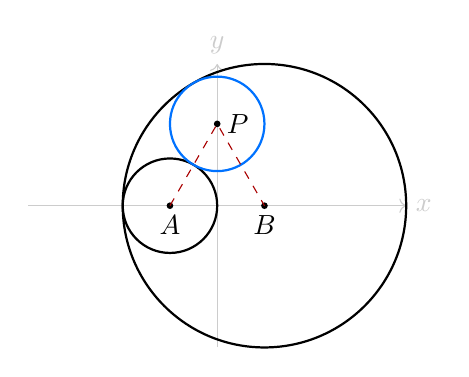
\begin{tikzpicture}[scale=0.6, baseline=(current bounding box.north)]
		\draw[->, gray!40] (-4,0) -- (4,0) node[right] {$x$};
		\draw[->, gray!40] (0,-3) -- (0,3) node[above] {$y$};
		
		% 圆 A
		\draw[thick] (-1,0) circle (1);
		\fill (-1,0) circle (2pt) node[below] {$A$};
		
		% 圆 B
		\draw[thick] (1,0) circle (3);
		\fill (1,0) circle (2pt) node[below] {$B$};
		
		% 动圆 P (示意，取椭圆上顶点 (0, sqrt(3)))
		% 此时 r=1. |PA|=2, |PB|=2.
		\coordinate (P) at (0, 1.732);
		\draw[thick, SkyBlue] (P) circle (1);
		\fill (P) circle (2pt) node[right] {$P$};
		
		% 连线
		\draw[dashed, DarkRed] (-1,0) -- (P) -- (1,0);
	\end{tikzpicture}
\end{minipage}

\category{相关点法求轨迹}
\begin{question}
	已知定点$B(3,0)$，$A$在$x^2+y^2=1$上运动，$\overrightarrow{AM}=\frac{1}{3}\overrightarrow{MB}$，求$M$轨迹.
\end{question}

\begin{minipage}[t]{0.7\textwidth}
	设$M(x,y), A(x_0,y_0)$.
	
	$\overrightarrow{AM}=(x-x_0, y-y_0), \quad \overrightarrow{MB}=(3-x, -y)$.
	
	由$\overrightarrow{AM}=\frac{1}{3}\overrightarrow{MB}$得：
	\[
	\begin{cases}
		x-x_0 = \frac{1}{3}(3-x) \\
		y-y_0 = \frac{1}{3}(-y)
	\end{cases}
	\implies
	\begin{cases}
		x_0 = \frac{4}{3}x - 1 \\
		y_0 = \frac{4}{3}y
	\end{cases}
	\]
	代入圆方程$x_0^2+y_0^2=1$：
	\[
	\left(\frac{4}{3}x-1\right)^2 + \left(\frac{4}{3}y\right)^2 = 1
	\]
	\[
	\frac{16}{9}\left(x-\frac{3}{4}\right)^2 + \frac{16}{9}y^2 = 1
	\]
	即$\left(x-\frac{3}{4}\right)^2 + y^2 = \frac{9}{16}$.
\end{minipage}
\hfill
\begin{minipage}[t]{0.3\textwidth}
	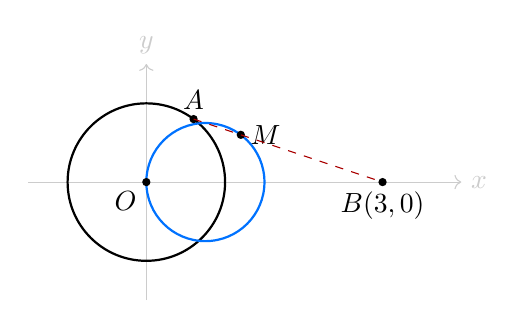
\begin{tikzpicture}[scale=1, baseline=(current bounding box.north)]
		\draw[->, gray!40] (-1.5,0) -- (4,0) node[right] {$x$};
		\draw[->, gray!40] (0,-1.5) -- (0,1.5) node[above] {$y$};
		
		% 圆 A (单位圆)
		\draw[thick] (0,0) circle (1);
		
		% 轨迹圆 M
		\draw[thick, SkyBlue] (0.75,0) circle (0.75);
		
		% 点
		\coordinate (B) at (3,0);
		\coordinate (A) at (0.6, 0.8); % 在单位圆上
		% M = 0.75*A + 0.25*B
		\coordinate (M) at ({0.75*0.6 + 0.25*3}, {0.75*0.8}); 
		
		\fill (0,0) circle (1.5pt) node[below left] {$O$};
		\fill (B) circle (1.5pt) node[below] {$B(3,0)$};
		\fill (A) circle (1.5pt) node[above] {$A$};
		\fill (M) circle (1.5pt) node[right] {$M$};
		
		\draw[dashed, DarkRed] (A) -- (M) -- (B);
	\end{tikzpicture}
\end{minipage}

\subsection{第九讲\quad 弦长问题}

\begin{knowledge}{直线与圆锥曲线的位置关系}
	联立直线与圆锥曲线方程，消元得到一元二次方程，通过判别式$\Delta$判定位置关系。
	\begin{itemize}
		\item $\Delta>0$：两个交点（相交）
		\item $\Delta=0$：一个交点（相切）
		\item $\Delta<0$：无交点（相离）
	\end{itemize}
\end{knowledge}

\subsubsection{直线与椭圆}
\begin{knowledge}{直线与椭圆联立}
	直线方程：$y=kx+m$
	椭圆方程：$b^2x^2+a^2y^2-a^2b^2=0$（化简式）
	
	联立消$y$：
	\[
	b^2x^2+a^2(kx+m)^2-a^2b^2=0
	\]
	整理得：
	\[
	(b^2+a^2k^2)x^2+2a^2kmx+a^2(m^2-b^2)=0
	\]
\end{knowledge}

\begin{question}
	直线$y=kx+2$与椭圆$x^2+\dfrac{y^2}{4}=1$的公共点个数？
\end{question}

\begin{minipage}[t]{0.7\textwidth}
	化简椭圆方程：$4x^2+y^2-4=0$
	
	联立：
	\[
	\begin{cases}
		y=kx+2 \\
		4x^2+y^2-4=0
	\end{cases}
	\]
	
	代入消元：$4x^2+(kx+2)^2-4=0$
	
	$4x^2+k^2x^2+4kx+4-4=0$
	
	$(4+k^2)x^2+4kx=0$
	
	$\Delta=(4k)^2-4(4+k^2)\cdot 0=16k^2\geq 0$
	
	$\therefore$ 恒有$1$或$2$个公共点。
\end{minipage}
\hfill
\begin{minipage}[t]{0.3\textwidth}
	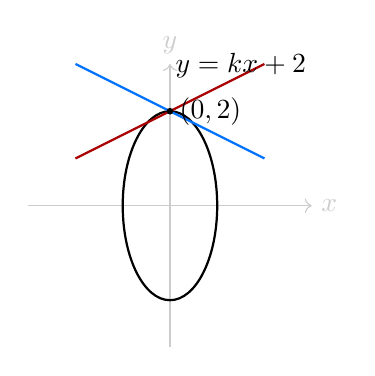
\begin{tikzpicture}[scale=0.6, baseline=(current bounding box.north)]
		\draw[->, gray!40] (-3,0) -- (3,0) node[right] {$x$};
		\draw[->, gray!40] (0,-3) -- (0,3) node[above] {$y$};
		
		% 椭圆 x^2 + y^2/4 = 1
		\draw[thick] (0,0) ellipse (1 and 2);
		
		% 直线 y=kx+2 (过点(0,2))
		\draw[thick, DarkRed] (-2,1) -- (2,3);
		\draw[thick, SkyBlue] (-2,3) -- (2,1);
		
		\fill (0,2) circle (2pt) node[right] {$(0,2)$};
		
		\node[above] at (1.5,2.5) {$y=kx+2$};
	\end{tikzpicture}
\end{minipage}

\subsubsection{直线与抛物线}
\begin{knowledge}{直线与抛物线联立}
	直线方程：$y=kx+m$
	抛物线方程：$y^2=2px$
	
	联立消$x$或$y$：
	\[
	k^2x^2+(2km-2p)x+m^2=0
	\]
	
	分类讨论：
	\begin{enumerate}[label=\arabic*.]
		\item $k=0$：一交点
		\item $k\neq 0$，$\Delta\geq 0$：两交点
	\end{enumerate}
\end{knowledge}

\begin{question}
	过定点$P(0,1)$且与抛物线$y^2=2x$只有一交点的直线方程为？
\end{question}

\begin{minipage}[t]{0.7\textwidth}
	\textbf{情况1：}$k$不存在，即$x=0$（竖直线）
	
	\textbf{情况2：}设$y=kx+b$，代入$P(0,1)\implies b=1$，$\therefore y=kx+1$
	
	联立抛物线：
	\[
	\begin{cases}
		y=kx+1 \\
		y^2=2x
	\end{cases}
	\]
	
	代入消元：$(kx+1)^2=2x$
	
	$k^2x^2+2kx+1=2x$
	
	$k^2x^2+(2k-2)x+1=0$
	
	$\Delta=(2k-2)^2-4k^2\cdot 1=0$
	
	$4k^2-8k+4-4k^2=0$
	
	$-8k+4=0\implies k=\dfrac{1}{2}$
	
	$\therefore$ 直线方程为$y=\dfrac{1}{2}x+1$或$x=0$。
\end{minipage}
\hfill
\begin{minipage}[t]{0.3\textwidth}
	\begin{tikzpicture}[scale=0.6, baseline=(current bounding box.north)]
		\draw[->, gray!40] (-1,0) -- (4,0) node[right] {$x$};
		\draw[->, gray!40] (0,-2) -- (0,3) node[above] {$y$};
		
		% 抛物线 y^2=2x
		\draw[thick, domain=0:3, smooth, variable=\y] plot ({0.5*\y*\y}, {\y});
		\draw[thick, domain=0:3, smooth, variable=\y] plot ({0.5*\y*\y}, {-\y});
		
		% 切线 y=0.5x+1
		\draw[thick, DarkRed] (-1,0.5) -- (3,2.5);
		
		% 竖直线 x=0
		\draw[thick, SkyBlue] (0,-2) -- (0,3);
		
		\fill (0,1) circle (2pt) node[left] {$P(0,1)$};
		\fill (2,2) circle (2pt) node[right] {切点};
	\end{tikzpicture}
\end{minipage}

\subsubsection{直线与双曲线}
\begin{knowledge}{直线与双曲线联立}
	直线方程：$y=kx+m$
	双曲线方程：$b^2x^2-a^2y^2-a^2b^2=0$
	
	联立消$y$：
	\[
	(b^2-a^2k^2)x^2-2a^2kmx-a^2(m^2+b^2)=0
	\]
	
	分类讨论：
	\begin{enumerate}[label=\arabic*.]
		\item 当$b^2-a^2k^2=0$，即$k=\pm\dfrac{b}{a}$时（渐近线斜率）
		\begin{itemize}
			\item $m=0$：无根，$y=\pm\dfrac{b}{a}x$为渐近线
			\item $m\neq 0$：一交点，$y=\pm\dfrac{b}{a}x+m$
		\end{itemize}
		\item $b^2-a^2k^2\neq 0$，$\Delta\geq 0$
	\end{enumerate}
	
	当$\Delta=0$时：
	\begin{enumerate}[label=\arabic*.]
		\item 一左一右：$x_1\cdot x_2<0$
		\item 右支：$\begin{cases} x_1\cdot x_2>0 \\ x_1+x_2>0 \end{cases}$
		\item 左支：$\begin{cases} x_1\cdot x_2>0 \\ x_1+x_2<0 \end{cases}$
	\end{enumerate}
\end{knowledge}

\category{直线与双曲线位置关系}
\begin{question}
	直线$y=kx+2$与双曲线$x^2-y^2=6$的右支交于不同两点，那么$k$的范围？
\end{question}

\begin{minipage}[t]{0.7\textwidth}
	联立：
	\[
	\begin{cases}
		y=kx+2 \\
		x^2-y^2-6=0
	\end{cases}
	\]
	
	代入消元：$x^2-(kx+2)^2-6=0$
	
	$x^2-(k^2x^2+4kx+4)-6=0$
	
	$(1-k^2)x^2-4kx-10=0$
	
	条件：
	\[
	\begin{cases}
		1-k^2\neq 0 \implies k\neq \pm 1 \\
		\Delta>0 \\
		x_1+x_2>0 \quad\text{(右支)} \\
		x_1\cdot x_2>0 \quad\text{(同侧)}
	\end{cases}
	\]
	
	$\Delta=(-4k)^2-4(1-k^2)(-10)>0$
	
	$16k^2+40(1-k^2)>0$
	
	$16k^2+40-40k^2>0$
	
	$40-24k^2>0$
	
	$k^2<\dfrac{5}{3}$
	
	由韦达定理：
	\[
	\begin{cases}
		x_1+x_2=\dfrac{4k}{1-k^2}>0 \\
		x_1\cdot x_2=\dfrac{-10}{1-k^2}>0
	\end{cases}
	\]
	
	$\therefore 1-k^2<0\implies k^2>1$
	
	结合$k^2<\dfrac{5}{3}$，得$1<k^2<\dfrac{5}{3}$
	
	$\therefore k\in\left(-\dfrac{\sqrt{15}}{3},-1\right)\cup\left(1,\dfrac{\sqrt{15}}{3}\right)$
\end{minipage}
\hfill
\begin{minipage}[t]{0.3\textwidth}
	\begin{tikzpicture}[scale=0.5, baseline=(current bounding box.north)]
		\draw[->, gray!40] (-4,0) -- (4,0) node[right] {$x$};
		\draw[->, gray!40] (0,-4) -- (0,4) node[above] {$y$};
		
		% 双曲线 x^2-y^2=6，用y作自变量避免断点
		\draw[thick, domain=-3.5:3.5, smooth, samples=200, variable=\y] plot ({sqrt(\y*\y+6)}, {\y});
		\draw[thick, domain=-3.5:3.5, smooth, samples=200, variable=\y] plot ({-sqrt(\y*\y+6)}, {\y});
		
		% 渐近线 y=x 和 y=-x
		\draw[dashed, gray] (-3.5,-3.5) -- (3.5,3.5);
		\draw[dashed, gray] (-3.5,3.5) -- (3.5,-3.5);
		
		% 直线 y=kx+2 (示意)
		\draw[thick, DarkRed] (-2,0) -- (3,3.5);
		
		\fill (0,2) circle (2pt) node[left] {$(0,2)$};
		
		\node[right] at (3,2) {右支};
	\end{tikzpicture}
\end{minipage}

\subsubsection{弦长问题}
\begin{knowledge}{弦长公式与通用步骤}
	$A,B$为在直线（斜率为$k$）上不同两点.
	
	弦长公式：$|AB|=\sqrt{1+k^2}\,|x_1-x_2|$.
	
	\begin{enumerate}[label=\arabic*.]
		\item 设直线方程，设$k$，讨论斜率是否存在.
		
		\item 联立.
		
		\item 设交点$A(x_1,y_1), B(x_2,y_2)$，列出$\Delta$，$x_1+x_2=-\dfrac{b}{a}$，$x_1x_2=\dfrac{c}{a}$.
		
		\item 弦长公式$AB=\sqrt{1+k^2}\sqrt{(x_1+x_2)^2-4x_1x_2}$，用$\dfrac{b}{a},\dfrac{c}{a}$代换.
		
	\end{enumerate}
\end{knowledge}

\category{焦点弦}
\begin{question}
	已知$\dfrac{x^2}{9}+y^2=1$，过左焦点$F$作倾斜角为$\dfrac{\pi}{6}$的直线交椭圆于$A,B$，则$|AB|=$?
\end{question}

\begin{minipage}[t]{0.7\textwidth}
	$a^2=9, b^2=1, c^2=8$.
	
	$\therefore F(-2\sqrt{2},0)$，$k=\tan\dfrac{\pi}{6}=\dfrac{\sqrt{3}}{3}$.
	
	$y-0=\dfrac{\sqrt{3}}{3}(x+2\sqrt{2}) \implies y=\dfrac{\sqrt{3}}{3}x+\dfrac{2\sqrt{6}}{3}$.
	
	联立$\begin{cases} y=\dfrac{\sqrt{3}}{3}x+\dfrac{2\sqrt{6}}{3} \\ x^2+9y^2-9=0 \end{cases} \implies 4x^2+12\sqrt{2}x+15=0$.
	
	设$A(x_1,y_1), B(x_2,y_2)$，$\Delta=48>0$.
	
	$x_1+x_2=-3\sqrt{2}$，$x_1x_2=\dfrac{15}{4}$.
	
	$AB=\sqrt{1+k^2}|x_1-x_2|=\sqrt{1+k^2}\sqrt{(x_1+x_2)^2-4x_1x_2}=\sqrt{\dfrac{4}{3}}\times\sqrt{3}=2$.
\end{minipage}
\hfill
\begin{minipage}[t]{0.3\textwidth}
	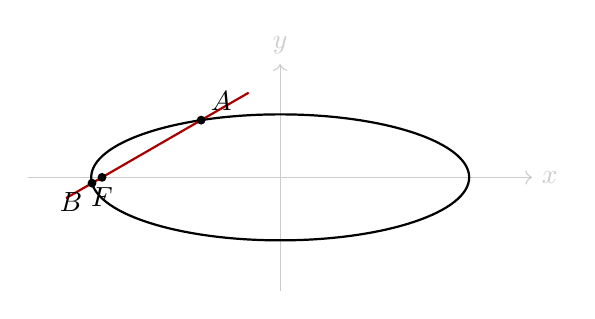
\begin{tikzpicture}[scale=0.8, baseline=(current bounding box.north)]
		\draw[->, gray!40] (-4,0) -- (4,0) node[right] {$x$};
		\draw[->, gray!40] (0,-1.8) -- (0,1.8) node[above] {$y$};
		\draw[thick] (0,0) ellipse (3 and 1);
		\pgfmathsetmacro{\xA}{(-3*sqrt(2)+sqrt(3))/2}
		\pgfmathsetmacro{\yA}{sqrt(3)/3*\xA+2*sqrt(6)/3}
		\pgfmathsetmacro{\xB}{(-3*sqrt(2)-sqrt(3))/2}
		\pgfmathsetmacro{\yB}{sqrt(3)/3*\xB+2*sqrt(6)/3}
		\coordinate (F) at ({-2*sqrt(2)},0);
		\coordinate (A) at (\xA,\yA);
		\coordinate (B) at (\xB,\yB);
		\draw[thick, DarkRed] ({-3.4},{sqrt(3)/3*(-3.4+2*sqrt(2))}) -- ({-0.5},{sqrt(3)/3*(-0.5+2*sqrt(2))});
		\fill (F) circle (2pt) node[below] {$F$};
		\fill (A) circle (2pt) node[above right] {$A$};
		\fill (B) circle (2pt) node[below left] {$B$};
	\end{tikzpicture}
\end{minipage}

\category{弦长求参数}
\begin{question}
	已知$\dfrac{x^2}{4}+y^2=1$，直线为$y=2x+m$，当$m=$?时，直线$l$被截得弦长为$\dfrac{20}{17}$.
\end{question}

\begin{minipage}[t]{0.7\textwidth}
	联立$\begin{cases} y=2x+m \\ x^2+4y^2-4=0 \end{cases} \implies 17x^2+16mx+4m^2-4=0$.
	
	设交点$A(x_1,y_1), B(x_2,y_2)$，$\Delta=16(17-m^2)>0$.
	
	$x_1+x_2=-\dfrac{16m}{17}$，$x_1x_2=\dfrac{4m^2-4}{17}$.
	
	$AB=\sqrt{1+k^2}|x_1-x_2|=\sqrt{1+k^2}\sqrt{(x_1+x_2)^2-4x_1x_2}=\dfrac{20}{17}$.
	
	即$\sqrt{5}\cdot\dfrac{\sqrt{16(17-m^2)}}{17}=\dfrac{20}{17}$.
	
	$\therefore m^2=12$，$m=\pm2\sqrt{3}$.
\end{minipage}
\hfill
\begin{minipage}[t]{0.3\textwidth}
	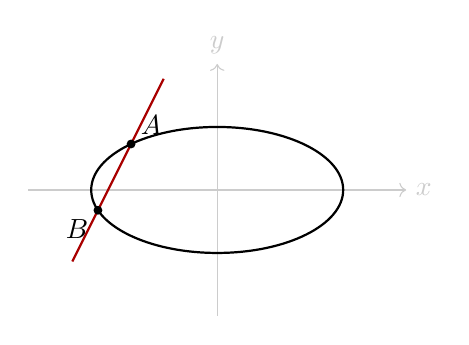
\begin{tikzpicture}[scale=0.8, baseline=(current bounding box.north)]
		\draw[->, gray!40] (-3,0) -- (3,0) node[right] {$x$};
		\draw[->, gray!40] (0,-2) -- (0,2) node[above] {$y$};
		\draw[thick] (0,0) ellipse (2 and 1);
		\pgfmathsetmacro{\m}{2*sqrt(3)}
		\pgfmathsetmacro{\xA}{(-16*sqrt(3)+2*sqrt(5))/17}
		\pgfmathsetmacro{\yA}{2*\xA+\m}
		\pgfmathsetmacro{\xB}{(-16*sqrt(3)-2*sqrt(5))/17}
		\pgfmathsetmacro{\yB}{2*\xB+\m}
		\coordinate (A) at (\xA,\yA);
		\coordinate (B) at (\xB,\yB);
		\draw[thick, DarkRed] ({-2.3},{2*(-2.3)+\m}) -- ({-0.85},{2*(-0.85)+\m});
		\fill (A) circle (2pt) node[above right] {$A$};
		\fill (B) circle (2pt) node[below left] {$B$};
	\end{tikzpicture}
\end{minipage}

\subsection{第十讲\quad 面积问题}

\subsubsection{面积计算问题}
\begin{knowledge}{面积计算通用步骤}
	前三步一样（与弦长问题同）.
	
	在算$AB$时，不先把$\sqrt{1+k^2}$算出.
	
	$|AB|=\sqrt{1+k^2}\cdot|x_1-x_2|=\sqrt{1+k^2}\cdot\sqrt{(x_1+x_2)^2-4x_1x_2}=\sqrt{1+k^2}\cdot\dfrac{\sqrt{\Delta}}{|a|}$.
	
	$d=\dfrac{|Ax_0+By_0+C|}{\sqrt{A^2+B^2}}\ \left(=\dfrac{|Ax_0+By_0+C|}{\sqrt{1+k^2}}\right)$.
	
	$\therefore S=\dfrac{1}{2}AB\cdot d=\dfrac{1}{2}\cdot\dfrac{\sqrt{\Delta}}{|a|}\cdot|Ax_0+By_0+C|$.
\end{knowledge}

\category{焦点三角形面积}
\begin{question}
	过椭圆$\dfrac{x^2}{4}+\dfrac{y^2}{3}=1$的左焦点$F_1$的直线$l$与椭圆相交于$A,B$，若$S_{\triangle AOB}=\dfrac{6\sqrt{2}}{7}$，则$O$到$l$距离为?
\end{question}

\begin{minipage}[t]{0.7\textwidth}
	\begin{enumerate}[label=\arabic*.]
		\item $k$不存在时，$S=\dfrac{1}{2}AB\cdot OF_1=\dfrac{1}{2}\cdot\dfrac{2b^2}{a}\cdot c=\dfrac{3}{2}\neq\dfrac{6\sqrt{2}}{7}$，不满足.
		
		\item $k$存在时，$y-0=k(x+1)$，即$y=kx+k$.
	\end{enumerate}
	
	联立$\begin{cases} y=kx+k \\ 3x^2+4y^2-12=0 \end{cases} \implies (4k^2+3)x^2+8k^2x+4k^2-12=0$.
	
	设$A(x_1,y_1), B(x_2,y_2)$，$\Delta=144k^2+144>0$.
	
	$x_1+x_2=-\dfrac{8k^2}{4k^2+3}$，$x_1x_2=\dfrac{4k^2-12}{4k^2+3}$.
	
	$AB=\sqrt{1+k^2}\cdot|x_1-x_2|=\sqrt{1+k^2}\cdot\dfrac{\sqrt{144k^2+144}}{4k^2+3}=\dfrac{12(k^2+1)}{4k^2+3}$.
	
	$d=\dfrac{|k\cdot0-0+k|}{\sqrt{k^2+1}}=\dfrac{|k|}{\sqrt{k^2+1}}$.
	
	$S=\dfrac{1}{2}AB\cdot d=\dfrac{6\sqrt{k^2+1}\cdot|k|}{4k^2+3}=\dfrac{6\sqrt{2}}{7}$.
	
	$\therefore k=\pm1$.
	
	代入$d=\dfrac{|k|}{\sqrt{k^2+1}}=\dfrac{\sqrt{2}}{2}$.
	
	
	
\end{minipage}
\hfill
\begin{minipage}[t]{0.3\textwidth}
	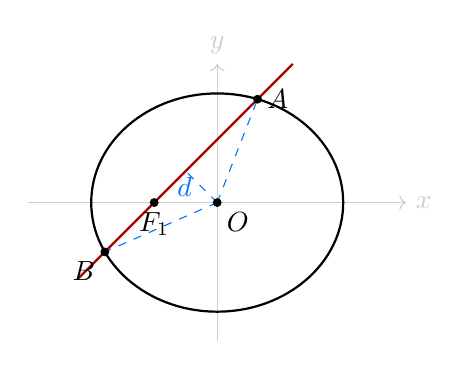
\begin{tikzpicture}[scale=0.8, baseline=(current bounding box.north)]
		\draw[->, gray!40] (-3,0) -- (3,0) node[right] {$x$};
		\draw[->, gray!40] (0,-2.2) -- (0,2.2) node[above] {$y$};
		\draw[thick] (0,0) ellipse (2 and {sqrt(3)});
		
		\pgfmathsetmacro{\xA}{(-4+6*sqrt(2))/7}
		\pgfmathsetmacro{\yA}{\xA+1}
		\pgfmathsetmacro{\xB}{(-4-6*sqrt(2))/7}
		\pgfmathsetmacro{\yB}{\xB+1}
		
		\coordinate (F) at (-1,0);
		\coordinate (O) at (0,0);
		\coordinate (A) at (\xA,\yA);
		\coordinate (B) at (\xB,\yB);
		
		% 直线 l: y=x+1 (k=1)
		\draw[thick, DarkRed] (-2.2,-1.2) -- (1.2,2.2);
		% 三角形 OAB
		\draw[dashed, SkyBlue] (O) -- (A);
		\draw[dashed, SkyBlue] (O) -- (B);
		% O 到 l 的距离 d
		\draw[dashed, SkyBlue] (O) -- (-0.5,0.5) node[midway, left] {$d$};
		
		\fill (F) circle (2pt) node[below] {$F_1$};
		\fill (O) circle (2pt) node[below right] {$O$};
		\fill (A) circle (2pt) node[right] {$A$};
		\fill (B) circle (2pt) node[below left] {$B$};
	\end{tikzpicture}
\end{minipage}

\subsection*{另解\quad 设 $l:\ x=ky-1$}

\textbf{说明：}此设法恒过 $F_1(-1,0)$，不能表示$y=0$，但这时$d=0$，明显不符合，排除情况.


\[\text{联立}
\begin{cases}
	x=ky-1\\[2pt]
	3x^2+4y^2-12=0
\end{cases}
\ \Longrightarrow\ (3k^2+4)y^2-6ky-9=0.
\]

设 $A(x_1,y_1)$，$B(x_2,y_2)$，则
\[
y_1+y_2=\frac{6k}{3k^2+4},\qquad y_1y_2=\frac{-9}{3k^2+4},
\]
\[
|y_1-y_2|=\sqrt{(y_1+y_2)^2-4y_1y_2}
=\frac{\sqrt{36k^2+36(3k^2+4)}}{3k^2+4}
=\frac{12\sqrt{k^2+1}}{3k^2+4}.
\]

以 $OF_1$ 为公共底（$|OF_1|=1$），两小三角形高分别为 $|y_1|,|y_2|$，故
\[
S_{\triangle AOB}=\frac12|OF_1|\cdot|y_1-y_2|
=\frac{6\sqrt{k^2+1}}{3k^2+4}=\frac{6\sqrt2}{7}.
\]

令 $t=\sqrt{k^2+1}\ (t\ge1)$，则 $3k^2+4=3t^2+1$，上式化为
\[
7t=\sqrt2\,(3t^2+1)\ \Longrightarrow\ 18t^4-37t^2+2=0
\ \Longrightarrow\ (t^2-2)(18t^2-1)=0.
\]
由 $t^2\ge1$ 得 $t^2=2$，即 $k^2=1$，$k=\pm1$.

直线 $l:\ x-ky+1=0$，故 $O$ 到 $l$ 的距离为$d=\dfrac{|0-k\cdot0+1|}{\sqrt{1+k^2}}=\dfrac{1}{\sqrt2}=\dfrac{\sqrt2}{2}.$

\subsection*{另解（约$\sqrt{k^2+1}$版）\quad 设 $l:\ x=ky-1$}

\textbf{可行性：}可以。此时 $|y_1-y_2|$ 同样可求弦长，且弦长公式中的 $\sqrt{1+k^2}$ 与距离公式分母中的 $\sqrt{1+k^2}$ 符号相消，无需真正算出它们。

由 $l:\ x-ky+1=0$（即 $A=1,\ B=-k,\ C=1$），有
\[
|AB|=\sqrt{1+k^2}\,|y_1-y_2|=\sqrt{1+k^2}\cdot\frac{\sqrt{\Delta}}{|a|},
\qquad
d=\frac{|Ax_0+By_0+C|}{\sqrt{1+k^2}},
\]
两式相乘，$\sqrt{1+k^2}$ 约去，故
\[
S_{\triangle AOB}=\frac12|AB|\cdot d
=\frac12\cdot\frac{\sqrt{\Delta}}{|a|}\cdot|Ax_0+By_0+C|.
\]

\textbf{代入计算：}将 $x=ky-1$ 代入 $3x^2+4y^2=12$：
\[
(3k^2+4)y^2-6ky-9=0,
\]
其中 $a=3k^2+4$，$\Delta=36k^2+36(3k^2+4)=144(k^2+1)$，$\sqrt\Delta=12\sqrt{k^2+1}$。

取 $(x_0,y_0)=(0,0)$，则 $|Ax_0+By_0+C|=|1|=1$，于是
\[
S=\frac12\cdot\frac{12\sqrt{k^2+1}}{3k^2+4}\cdot1
=\frac{6\sqrt{k^2+1}}{3k^2+4}=\frac{6\sqrt2}{7}.
\]

\textbf{解出 $k$：}去分母得 $7\sqrt{k^2+1}=\sqrt2\,(3k^2+4)$。令 $u=k^2+1\ (u\ge1)$，则 $3k^2+4=3u+1$：
\[
49u=2(3u+1)^2\ \Longrightarrow\ 18u^2-37u+2=0
\ \Longrightarrow\ (u-2)(18u-1)=0,
\]
由 $u\ge1$ 得 $u=2$，即 $k^2=1$。

\textbf{回代求距离：}
\[
d=\frac{|Ax_0+By_0+C|}{\sqrt{1+k^2}}=\frac{1}{\sqrt2}=\frac{\sqrt2}{2}.
\]

\textbf{注：}此写法的好处是 $\sqrt{1+k^2}$ 在 $S$ 的表达式中已先行约去，全程只需计算 $\dfrac{\sqrt\Delta}{|a|}$ 与距离公式的分子 $|Ax_0+By_0+C|$（本题该分子恰为 $1$），不必分别求出 $|AB|$ 与 $d$ 再相乘，运算量小。

\subsubsection{面积最值问题}
\begin{knowledge}{面积最值的两类函数型}
	
	\begin{minipage}{0.6\textwidth}
	\begin{enumerate}[label=\arabic*.]
	\item 二次函数型：$S=|m|\cdot\sqrt{9-m^2}$.
	
	令$m^2=t,\ t>0$.
	
	$\therefore S=\sqrt{(9-t)t}=\sqrt{-t^2+9t}$.
	
	在$t=\dfrac{9}{2}$时，$S_{\max}$.
	
	
	\item 分式型：$S=\dfrac{4k^2+3}{\sqrt{4k^2+1}}$.
	
	令$\sqrt{4k^2+1}=t,\ t\geq1$.
	
	$S=\dfrac{t^2+2}{t}=t+\dfrac{2}{t}$.
	
	当$t=\sqrt{2}$时，$S_{\min}$（对勾函数）.
	\end{enumerate}
	\end{minipage}
	\hfill
	\begin{minipage}{0.4\textwidth}
	
		\begin{tikzpicture}[scale=0.5, baseline=(current bounding box.north)]
			\begin{scope}[shift={(0,0)}]
				\draw[->, gray!40] (0,0) -- (4,0) node[right] {$t$};
				\draw[->, gray!40] (0,0) -- (0,5) node[above] {$S$};
				\draw[thick, DarkRed, domain=0.45:3.6, smooth, variable=\t] plot ({\t}, {\t+2/\t});
				\fill[DarkRed] ({sqrt(2)}, {2*sqrt(2)}) circle (2pt);
				\draw[dashed, SkyBlue] ({sqrt(2)},0) -- ({sqrt(2)},{2*sqrt(2)});
				\node[below] at ({sqrt(2)},0) {$\sqrt{2}$};
			\end{scope}
			\begin{scope}[shift={(0,-10)}]
				\draw[->, gray!40] (0,0) -- (4.5,0) node[right] {$t$};
				\draw[->, gray!40] (0,0) -- (0,6) node[above] {$S$};
				\draw[thick, DarkRed, domain=1:4, smooth, variable=\t] plot ({\t}, {\t+4/\t});
				\fill[DarkRed] (2,4) circle (2pt);
				\draw[dashed, SkyBlue] (2,0) -- (2,4);
				\node[below] at (2,0) {$2$};
			\end{scope}
		\end{tikzpicture}
	
	\end{minipage}
\end{knowledge}

\category{面积最大值}
\begin{question}
	已知$A(0,-2)$，椭圆$\dfrac{x^2}{4}+y^2=1$，过$A$直线$l$与椭圆交于$P,Q$，则$\triangle OPQ$面积最大值?
\end{question}

\begin{minipage}[t]{0.7\textwidth}
	\begin{enumerate}[label=\arabic*.]
		\item $k$不存在时，不满足.
		
		\item $k$存在时，$y=kx-2$.
	\end{enumerate}
	
	联立$\begin{cases} y=kx-2 \\ x^2+4y^2-4=0 \end{cases} \implies (4k^2+1)x^2-16kx+12=0$.
	
	设$P(x_1,y_1), Q(x_2,y_2)$，$\Delta=64k^2-48>0$.
	
	$x_1+x_2=\dfrac{16k}{4k^2+1}$，$x_1x_2=\dfrac{12}{4k^2+1}$.
	
	$PQ=\sqrt{1+k^2}\cdot|x_1-x_2|=\sqrt{1+k^2}\cdot\dfrac{\sqrt{64k^2-48}}{4k^2+1}$.
	
	$d=\dfrac{|k\cdot0-0-2|}{\sqrt{k^2+1}}=\dfrac{2}{\sqrt{k^2+1}}$.
	
	$S=\dfrac{1}{2}\cdot PQ\cdot d=\dfrac{4\sqrt{4k^2-3}}{4k^2+1}$.
	
	令$t=\sqrt{4k^2-3},\ t>0$.
	
	$S=\dfrac{4t}{t^2+4}=\dfrac{4}{t+\dfrac{4}{t}}$.
	
	当$t=2$时，$\left(t+\dfrac{4}{t}\right)_{\min}=4$.
	
	$\therefore S_{\max}=1$.
\end{minipage}
\hfill
\begin{minipage}[t]{0.3\textwidth}
	\begin{tikzpicture}[scale=0.8, baseline=(current bounding box.north)]
		\draw[->, gray!40] (-3,0) -- (3,0) node[right] {$x$};
		\draw[->, gray!40] (0,-2.6) -- (0,2) node[above] {$y$};
		\draw[thick] (0,0) ellipse (2 and 1);
		
		\coordinate (O) at (0,0);
		\coordinate (A) at (0,-2);
		\coordinate (P) at (2,0);
		\coordinate (Q) at (1.2,-0.8);
		
		% 直线 l: y=x-2 (k=1)
		\draw[thick, DarkRed] (-0.5,-2.5) -- (2.5,0.5);
		\draw[dashed, SkyBlue] (O) -- (P);
		\draw[dashed, SkyBlue] (O) -- (Q);
		
		\fill (O) circle (2pt) node[above left] {$O$};
		\fill (A) circle (2pt) node[left] {$A(0,-2)$};
		\fill (P) circle (2pt) node[above right] {$P$};
		\fill (Q) circle (2pt) node[below left] {$Q$};
	\end{tikzpicture}
\end{minipage}

\subsection{第十一讲\quad 定值问题}
\begin{knowledge}{定值问题通用步骤}
	\begin{enumerate}[label=\arabic*.]
		\item 设直线方程：1.存在 \quad 2.不存在（提前写答案）.
		
		\item 联立（消$y$）：$Ax^2+Bx+C=0$.
		
		\item 设$A(x_1,y_1), B(x_2,y_2)$，$\Delta>0$（不算），求$x_1x_2$，$x_1+x_2$.
		
		\item 定值：核心条件转化.
		\begin{itemize}
			\item 斜率（$k=\tan\alpha$）
			\item 向量（$\overrightarrow{a}\cdot\overrightarrow{b}=0$，$\perp$）
			\item 两点距
		\end{itemize}
	\end{enumerate}
	
	附：整理后再代入韦达定理；遇$y$代入解析式；在通分前分离常数.
	
	目标：韦达定理.
	
	\textbf{技巧：}若第一问的答案已知，可只算分母.
\end{knowledge}

\category{向量定值}
\begin{question}
	已知$\dfrac{x^2}{4}+\dfrac{y^2}{2}=1$（$a^2=4, b^2=2 \implies c^2=2$），过$P(0,1)$的直线交于$A,B$，证明$\overrightarrow{OA}\cdot\overrightarrow{OB}+\overrightarrow{PA}\cdot\overrightarrow{PB}$为定值.
\end{question}

\begin{minipage}[t]{0.7\textwidth}
	1. $k$不存在（一条竖线），$A(0,\sqrt{2}), B(0,-\sqrt{2})$.
	
	$\overrightarrow{OA}\cdot\overrightarrow{OB}=-2$，$\overrightarrow{PA}\cdot\overrightarrow{PB}=-1$.
	
	$\therefore \overrightarrow{OA}\cdot\overrightarrow{OB}+\overrightarrow{PA}\cdot\overrightarrow{PB}=-3$.
	
	2. 当$k$存在时，$y-1=kx$.
	
	联立$\begin{cases} y=kx+1 \\ x^2+2y^2-4=0 \end{cases} \implies (2k^2+1)x^2+4kx-2=0$.
	
	设$A(x_1,y_1), B(x_2,y_2)$，$\Delta>0$.
	
	$x_1+x_2=\dfrac{-4k}{2k^2+1}$，$x_1x_2=\dfrac{-2}{2k^2+1}$.
	
	$\overrightarrow{PA}=(x_1,kx_1)$，$\overrightarrow{PB}=(x_2,kx_2)$.
	
	$\therefore \overrightarrow{OA}\cdot\overrightarrow{OB}+\overrightarrow{PA}\cdot\overrightarrow{PB}$
	$=x_1x_2+(kx_1+1)(kx_2+1)+x_1x_2+k^2x_1x_2$
	$=(2k^2+2)\cdot\dfrac{-2}{2k^2+1}+k\cdot\dfrac{-4k}{2k^2+1}+1$
	$=\dfrac{-8k^2-4}{2k^2+1}+1=-3$.
	
	$\therefore$ 定值为$-3$.
\end{minipage}
\hfill
\begin{minipage}[t]{0.3\textwidth}
	\begin{tikzpicture}[scale=0.8, baseline=(current bounding box.north)]
		\draw[->, gray!40] (-3,0) -- (3,0) node[right] {$x$};
		\draw[->, gray!40] (0,-2) -- (0,2) node[above] {$y$};
		\draw[thick] (0,0) ellipse (2 and {sqrt(2)});
		
		\pgfmathsetmacro{\xA}{(-2+sqrt(10))/3}
		\pgfmathsetmacro{\yA}{\xA+1}
		\pgfmathsetmacro{\xB}{(-2-sqrt(10))/3}
		\pgfmathsetmacro{\yB}{\xB+1}
		
		\coordinate (P) at (0,1);
		\coordinate (A) at (\xA,\yA);
		\coordinate (B) at (\xB,\yB);
		\coordinate (O) at (0,0);
		
		% 直线 y=x+1 (k=1)
		\draw[thick, DarkRed] (-2.2,-1.2) -- (1.2,2.2);
		\draw[dashed, SkyBlue] (O) -- (A);
		\draw[dashed, SkyBlue] (O) -- (B);
		
		\fill (P) circle (2pt) node[left] {$P$};
		\fill (A) circle (2pt) node[right] {$A$};
		\fill (B) circle (2pt) node[below left] {$B$};
	\end{tikzpicture}
\end{minipage}

\category{角度定值（抛物线）}
\begin{question}
	设抛物线$y^2=2x$，$A(2,0)$，$B(-2,0)$，过$A$直线$l$与抛物线交于$M,N$，证明$\angle ABM=\angle ABN$.
\end{question}

\begin{minipage}[t]{0.75\textwidth}
	分析：$\angle ABM=\angle ABN \iff \tan\angle ABM=\tan\angle ABN \iff k_{BM}=-k_{BN}$.
	
	$\therefore$ 需证$k_{BM}+k_{BN}=0$.
	
	设$l: x=my+2$，联立$y^2=2x$：
	\[
	y^2-2my-4=0
	\]
	设$M(x_1,y_1), N(x_2,y_2)$，则$y_1+y_2=2m$，$y_1y_2=-4$.
	
	$k_{BM}+k_{BN}=\dfrac{y_1}{x_1+2}+\dfrac{y_2}{x_2+2}=\dfrac{y_1(my_2+4)+y_2(my_1+4)}{(my_1+4)(my_2+4)}$
	$=\dfrac{2my_1y_2+4(y_1+y_2)}{(my_1+4)(my_2+4)}=\dfrac{-8m+8m}{(my_1+4)(my_2+4)}=0$.
	
	$\therefore \angle ABM=\angle ABN$.
\end{minipage}
\hfill
\begin{minipage}[t]{0.3\textwidth}
	\begin{tikzpicture}[scale=0.7, baseline=(current bounding box.north)]
		\draw[->, gray!40] (-3,0) -- (4,0) node[right] {$x$};
		\draw[->, gray!40] (0,-3) -- (0,3) node[above] {$y$};
		% 抛物线 y^2=2x
		\draw[thick, domain=-2.6:2.6, smooth, variable=\y] plot ({0.5*\y*\y}, {\y});
		
		\pgfmathsetmacro{\yM}{(1+sqrt(17))/2}
		\pgfmathsetmacro{\xM}{0.5*\yM*\yM}
		\pgfmathsetmacro{\yN}{(1-sqrt(17))/2}
		\pgfmathsetmacro{\xN}{0.5*\yN*\yN}
		
		\coordinate (A) at (2,0);
		\coordinate (B) at (-2,0);
		\coordinate (M) at (\xM,\yM);
		\coordinate (N) at (\xN,\yN);
		
		% 直线 l 过 A
		\draw[thick, DarkRed] (N) -- (M);
		% BM, BN
		\draw[thick, SkyBlue] (B) -- (M);
		\draw[thick, SkyBlue] (B) -- (N);
		
		\fill (A) circle (2pt) node[below right] {$A$};
		\fill (B) circle (2pt) node[above left] {$B$};
		\fill (M) circle (2pt) node[right] {$M$};
		\fill (N) circle (2pt) node[right] {$N$};
	\end{tikzpicture}
\end{minipage}

\subsection{第十二讲\quad 等差数列}

\subsubsection{数列的概念}
\begin{knowledge}{数列的概念}
	第$n$项$a_n$.
	
	$a_n$与$n$的关系可用一式子表示：$a_n=f(n)$，叫通项公式.
	
	数列不一定有通项公式.
	
	每个数列通项公式可能不唯一.
	
	递推公式：相邻多项关系可用一式子表示，如$1,1,2,3,5,8,13$：$1+1=2$，$1+2=3$，$2+3=5$.
	
	$S_n=a_1+\cdots+a_n$.
	
	按一定次序排列的一列数叫数列.
	
	分类：
	\begin{itemize}
		\item 有穷数列、无穷数列.
		
		\item 递增数列、递减数列.
		
		\item 周期数列.
		
		\item 常数数列、摆动数列.
		
	\end{itemize}
\end{knowledge}

\subsubsection{等差数列的概念}
\begin{knowledge}{等差数列的概念与公式}
	等差：后一项与前一项的差为常数（公差$d$）.
	
	等差中项：$a,b,c \implies 2b=a+c$.
	
	通项公式（累加法）：
	\[
	\begin{cases}
		a_2-a_1=d \\
		a_3-a_2=d \\
		a_4-a_3=d \\
		\vdots \\
		a_n-a_{n-1}=d
	\end{cases}
	\implies a_n-a_1=(n-1)d
	\]
	
	$\bigstar \ a_n=a_1+(n-1)d$，$a_n=a_m+(n-m)d$（基本量）.
	
	$\bigstar ~ S_n=na_1+\dfrac{n(n-1)}{2}d$.
	
	$S_n=\dfrac{d}{2}n^2+\left(a_1-\dfrac{d}{2}\right)n$.
	
	在知末项时，用$S_n=\dfrac{(a_1+a_n)n}{2}$（首+末）$\times$项数$\div 2$.
\end{knowledge}

\category{等差中项}
\begin{question}
	在$\{a_n\}$中，$a_2=2$，$a_6=0$，且$\left\{\dfrac{1}{a_n+1}\right\}$为等差数列，$a_4=$?
\end{question}

由等差中项：
\[
\frac{1}{a_2+1}+\frac{1}{a_6+1}=2\cdot\frac{1}{a_4+1}.
\]

即$\dfrac{1}{3}+1=\dfrac{2}{a_4+1}$.

$\dfrac{4}{3}=\dfrac{2}{a_4+1} \implies a_4+1=\dfrac{3}{2}$.

$\therefore a_4=\dfrac{1}{2}$.

\category{等差性质与前$n$项和}
\begin{question}
	若$a_1=1$，$a_{m-1}+a_m+a_{m+1}=27$，$S_m=45$，求$m$.
\end{question}

由等差数列性质：$a_{m-1}+a_{m+1}=2a_m$.

$\therefore 3a_m=27 \implies a_m=9$.

在知末项时，用$S_m=\dfrac{(a_1+a_m)m}{2}$.

$S_m=\dfrac{(1+9)m}{2}=45 \implies 5m=45$.

$\therefore m=9$.

\subsubsection{等差数列的性质}
\begin{knowledge}{等差数列的性质}
	
	$\bigstar ~p+t=m+n \implies a_p+a_t=a_m+a_n$（两边项数相同）.
	
	$S_{2n-1}=\dfrac{(a_1+a_{2n-1})\cdot(2n-1)}{2}=(2n-1)a_n$.
	
	eg：$S_{17}=17a_9$（$2n-1=17 \implies n=9$）.
	
	一条件：性质解题.
	
	两条件：基本量解题.
\end{knowledge}

\category{基本量解题}
\begin{question}
	$a_1+a_2+a_3=9$，$a_1$与$a_{11}$的等差中项是$15$，求$a_9$.
\end{question}

$3a_2=9 \implies a_2=3$.

等差中项：$a_1$与$a_{11} \implies \dfrac{1+11}{2}=6 \implies a_6=15$.

两个条件：$\begin{cases} a_6=a_1+5d \\ a_2=a_1+d \end{cases} \implies \begin{cases} a_1=0 \\ d=3 \end{cases}$.

$\therefore a_9=a_1+8d=24$.

\category{性质解题}
\begin{question}
	已知等差$\{a_n\}$，$a_2-a_5+a_8=4$，求$S_9$.
\end{question}

一条件：性质：$a_2+a_8=2a_5$.

$\therefore a_5=4$.

$S_9=9a_5=36$（$\dfrac{9+1}{2}=5$）.

\category{两等差数列和之比}
\begin{question}
	$\{a_n\},\{b_n\}$等差，$\dfrac{S_n}{T_n}=\dfrac{4n+2}{5n+2}$，求$\dfrac{a_5}{b_5}$.
\end{question}

$S_{2n-1}=(2n-1)a_n$.

$\therefore 2n-1=9 \implies n=5$.

$\therefore \dfrac{a_5}{b_5}=\dfrac{S_9}{T_9}=\dfrac{4\cdot9+2}{5\cdot9+2}=\dfrac{38}{47}$.

\category{乘1法最值}
\begin{question}
	$\{a_n\}$等差，$a_m+a_n=a_2+a_7$，求$\left(\dfrac{1}{m}+\dfrac{9}{n}\right)_{\min}$.
\end{question}

$m+n=9$.

$\left(\dfrac{1}{m}+\dfrac{9}{n}\right)(m+n)\cdot\dfrac{1}{9}=\left(10+\dfrac{n}{m}+\dfrac{9m}{n}\right)\times\dfrac{1}{9}$.

$m,n$是角标，需满足正整数，取等可能取不到.

$\dfrac{n}{m}=\dfrac{9m}{n} \implies n=3m$，结合$m+n=9 \implies m=\dfrac{9}{4},\ n=\dfrac{27}{4}$（非整数，舍）.

$\therefore$ 对正整数，比较$m=2$与$m=3$：

$m=2,\ n=7$：$\dfrac{1}{2}+\dfrac{9}{7}=\dfrac{25}{14}$.

$m=3,\ n=6$：$\dfrac{1}{3}+\dfrac{9}{6}=\dfrac{11}{6}$.

$\therefore$ 最小值为$\dfrac{25}{14}$.

\subsection{第十三讲\quad 等比数列}

\subsubsection{概念}
\begin{knowledge}{等比数列的概念}
	
	后一项比前一项为常数（公比$q$）；等比不能有$0$.
	
	等比中项：$x,G,y \implies G^2=xy$.
	
	通项公式：$a_n=a_1\cdot q^{n-1}=a_2\cdot q^{n-2}=a_3\cdot q^{n-3}$.
	
	累乘法：
	\[
	\begin{cases}
		\dfrac{a_2}{a_1}=q \\
		\dfrac{a_3}{a_2}=q \\
		\vdots \\
		\dfrac{a_n}{a_{n-1}}=q
	\end{cases}
	\implies \frac{a_n}{a_1}=q^{n-1}.
	\]
	
	判断数列方式：
	\begin{enumerate}[label=\arabic*.]
		\item 定义法：$a_{n+1}-a_n=$常：等差；$\dfrac{a_{n+1}}{a_n}=$常：等比.
		
		\item 等中项：$a_{n-1}+a_{n+1}=2a_n$等差；$a_{n-1}\cdot a_{n+1}=a_n^2$等比.
		
		\item 公式：根据题目表示出$a_n$（可能多项）；整理出：$An+B$等差；$C\cdot D^n$等比.
		
	\end{enumerate}
	
	常数列是等差；常数列除$0,0,0,\cdots$外是等比.
	
	前$n$项和（错位相减）：
	\[
	S_n=\begin{cases}
		na_1 & (q=1) \\
		\dfrac{a_1(1-q^n)}{1-q} & (q\neq 1)
	\end{cases}
	\]
\end{knowledge}

\category{分类讨论求通项}
\begin{question}
	等比$\{a_n\}$，$a_2=6$，$a_5-2a_4-a_3+12=0$，求$a_n$.
\end{question}

$a_2q^3-2a_2q^2-a_2q+12=0$.

$6q^3-12q^2-6q+12=0 \implies q^3-2q^2-q+2=0$.

$q^2(q-2)-(q-2)=0 \implies (q-2)(q^2-1)=0$.

$\therefore q=\pm1$或$2$.

\begin{enumerate}[label=\arabic*.]
	\item $q=2$：$a_n=a_2q^{n-2}=6\cdot2^{n-2}$.
	
	\item $q=1$：$a_n=a_2q^{n-2}=6$.
	
	\item $q=-1$：$a_n=a_2q^{n-2}=6\cdot(-1)^{n-2}$.
	
\end{enumerate}

\category{递推关系求项}
\begin{question}
	$\{a_n\}$满足$3a_{n+1}+a_n=0$，$a_2=-\dfrac{4}{3}$，求$a_{10}$.
\end{question}

$3a_{n+1}=-a_n$.

$\dfrac{a_{n+1}}{a_n}=-\dfrac{1}{3}$.

$\therefore q=-\dfrac{1}{3}$.

$a_{10}=a_2\cdot q^8=-\dfrac{4}{3}\cdot\dfrac{1}{3^8}=-4\times3^{-9}$.

\subsubsection{等比数列的性质}
\begin{knowledge}{等比数列的性质}
	$p+t=m+n \implies a_p\cdot a_t=a_m\cdot a_n$.
	
	若$2m=p+t$，则$a_p a_t=a_m^2$.
\end{knowledge}

\category{由通项判断数列类型}
\begin{question}
	$\{a_n\}$等比，$a_1=1$，$q=3$，求下列数列的通项公式：
	\begin{enumerate}[label=\arabic*.]
		\item $\left\{\dfrac{a_{n+1}}{a_n}\right\}$
		\item $\{a_{n+1}-a_n\}$
		\item $\{\log_3 a_n\}$
		\item $\{a_n\cdot a_{n+1}\}$
	\end{enumerate}
\end{question}

优先求出题目中$a_n$通项公式：$a_n=a_1\cdot q^{n-1}=3^{n-1}$.

\begin{enumerate}[label=\arabic*.]
	\item $\left\{\dfrac{a_{n+1}}{a_n}\right\}=\left\{\dfrac{a_n\cdot q}{a_n}\right\}=\{q\}=\{3\}$，常数列.
	
	\item $\{a_{n+1}-a_n\}=\{3^n-3^{n-1}\}=\{2\cdot3^{n-1}\}$，等比数列.
	
	\item $\{\log_3 a_n\}=\{\log_3 3^{n-1}\}=\{n-1\}$，等差数列.
	
	\item $\{a_n\cdot a_{n+1}\}=\{3^{n-1}\cdot3^n\}=\{3\cdot9^{n-1}\}$，等比数列.
	
\end{enumerate}

\subsubsection{等差、等比综合}
\begin{knowledge}{综合要点}
	
	分清等差等比.
	
	运用中项.
\end{knowledge}

\category{等差中项运用}
\begin{question}
	等比$\{a_n\}$，$3a_1,\ \dfrac{1}{2}a_3,\ 2a_2$等差，求$\dfrac{a_6}{a_4}$.
\end{question}

$3a_1+2a_2=2\times\dfrac{1}{2}a_3$.

$3a_1+2a_1q=a_1q^2 \implies q^2-2q-3=0$.

$q=3$或$-1$（舍）.

$\dfrac{a_6}{a_4}=q^2=9$.

\category{正项数列解方程}
\begin{question}
	$\{a_n\}$正，$a_2\cdot a_4=1$，$S_3=7$，求$S_5$.
\end{question}

$a_2\cdot a_4=a_3^2=a_1^2q^4=1 \implies a_1=\dfrac{1}{q^2}$.

$S_3=\dfrac{a_1(1-q^3)}{1-q}=\dfrac{\frac{1}{q^2}(1-q^3)}{1-q}=7$.

用立方差公式分解：
\[
\frac{\frac{1}{q^2}(1-q)(1+q+q^2)}{1-q}=7 \implies 1+q+q^2=7q^2.
\]

$6q^2-q-1=0 \implies q=\dfrac{1}{2},\ a_1=4$.

$\therefore S_5=\dfrac{4\left(1-\left(\frac{1}{2}\right)^5\right)}{1-\frac{1}{2}}=\dfrac{31}{4}$.

\category{根与性质运用}
\begin{question}
	等比$\{a_n\}$，$a_3,a_{15}$是方程$x^2-6x+8=0$两根，求$\dfrac{a_1a_{17}}{a_9}$.
\end{question}

由韦达定理：$a_3+a_{15}=6$，$a_3a_{15}=8$.

$a_1a_{17}=a_3a_{15}=8=a_9^2$.

$\because a_9=a_3q^6$，且$a_3>0$.

$\therefore a_9=2\sqrt{2}$.

$\therefore \dfrac{a_1a_{17}}{a_9}=\dfrac{8}{2\sqrt{2}}=2\sqrt{2}$.

\category{中项配方}
\begin{question}
	$\{a_n\}$等比，$a_n>0$，$a_2a_4+2a_3a_5+a_4a_6=25$，求$a_3+a_5$.
\end{question}

$a_2a_4=a_3^2$，$a_4a_6=a_5^2$.

$a_3^2+2a_3a_5+a_5^2=25 \implies (a_3+a_5)^2=25$.

$\because a_n>0$.

$\therefore a_3+a_5=5$.

\subsection{第十四讲\quad 数列求通项}

\subsubsection{累加法}
\begin{knowledge}{累加法}
	整理出能用累加消项的式子.
	
	如：$a_{n+1}-a_n=n+1$.
	
	找出与$n$同步变化的项：$a_n$角标.
	
	进行从小到大赋值，直到找到消项规律，整理式子（右边用$S_n$）.
	
	如$a_n-a_1=\cdots$（判断等差、等比）.
	
	把$a_1$移项：$a_n=\cdots$.
\end{knowledge}

\category{累加法}
\begin{question}
	$\{a_n\}$满足$a_1=1$，$\dfrac{1}{a_{n+1}}-\dfrac{1}{a_n}=4^n$，则求$a_n$通项公式.
\end{question}

$\begin{cases}
	\dfrac{1}{a_2}-\dfrac{1}{a_1}=4 \\
	\dfrac{1}{a_3}-\dfrac{1}{a_2}=4^2 \\
	\vdots \\
	\dfrac{1}{a_n}-\dfrac{1}{a_{n-1}}=4^{n-1}
\end{cases}$

累加：$\dfrac{1}{a_n}-\dfrac{1}{a_1}=4+4^2+\cdots+4^{n-1}$（等比）.

$S_n=\dfrac{4(1-4^{n-1})}{1-4}=\dfrac{4(4^{n-1}-1)}{3}=\dfrac{4^n-4}{3}$.

$\therefore \dfrac{1}{a_n}=1+\dfrac{4^n-4}{3}=\dfrac{4^n-1}{3}$.

$\therefore a_n=\dfrac{3}{4^n-1}$.

\subsubsection{累乘法}
\begin{knowledge}{累乘法}
	展开括号，合并同类项，整理出：
	
	单项$\dfrac{a_n}{a_{n+1}}=\dfrac{n}{n+1}$.
	
	找出同步变化的项.
	
	赋值，直到找到规律.
	
	运用$S_n$（判断等差等比）.
	
	把$a_1$乘过去：$\dfrac{a_n}{a_1}=S_n$.
\end{knowledge}

\category{等差与累加结合}
\begin{question}
	$\{a_n\}$首项为$3$，$\{b_n\}$等差，$b_n=a_{n+1}-a_n$，$b_3=-2$，$b_{10}=12$，求$a_8$.
\end{question}

两个条件：$\begin{cases} b_3=b_1+2d=-2 \\ b_{10}=b_1+9d=12 \end{cases} \implies \begin{cases} b_1=-6 \\ d=2 \end{cases}$.

$b_n=b_1+(n-1)d=2n-8$.

$\therefore a_{n+1}-a_n=2n-8$.

$\begin{cases}
	a_2-a_1=-6 \\
	a_3-a_2=-4 \\
	\vdots \\
	a_n-a_{n-1}=2n-10
\end{cases}$

累加：$a_n-a_1=-6-4+\cdots+(2n-10)=\dfrac{(-6+2n-10)(n-1)}{2}=(n-8)(n-1)$.

$a_n=3+(n-8)(n-1)$.

$\therefore a_8=3$.

\subsubsection{$a_n$与$S_n$的关系}
\begin{knowledge}{通用方法}
	题目给$S_n=\cdots a_n$.
	
	$S_{n-1}=\cdots a_{n-1}$.
	
	$S_n-S_{n-1}=a_n$.
	
	得到一个关于$a_n$的式子.
	
	使用累乘或累加化成$a_n=\cdots$.
\end{knowledge}

\category{$a_{n+1}=3S_n$型}
\begin{question}
	$\{a_n\}$，$a_1=1$，$a_{n+1}=3S_n\ (n\geq1)$，求$a_6$.
\end{question}

$a_n=3S_{n-1}\ (n\geq2)$（不一定代表从$a_2$开始的通项）.

$a_{n+1}-a_n=3(S_n-S_{n-1})\ (n\geq2)$.

$a_{n+1}-a_n=3a_n\ (n\geq2)$.

$a_{n+1}=4a_n\ (n\geq2)$.

$\{a_n\}$是从第二项开始公比为$4$的等比数列.

$a_2=3S_1=3$.

$\therefore a_n=a_2\cdot q^{n-2}=3\cdot4^{n-2}\ (n\geq2)$.

$a_1=1$不满足上式.

$\therefore a_n=\begin{cases} 1, & n=1 \\ 3\cdot4^{n-2}, & n\geq2 \end{cases}$.

$\therefore a_6=3\times4^4=768$.

\category{$na_{n+1}=2S_n$型}
\begin{question}
	$a_1=1$，$na_{n+1}=2S_n$，求通项公式.
\end{question}

$(n-1)a_n=2S_{n-1}\ (n\geq2)$.

两式相减：$na_{n+1}-(n-1)a_n=2a_n \implies na_{n+1}=(n+1)a_n\ (n\geq2)$.

$\dfrac{a_{n+1}}{a_n}=\dfrac{n+1}{n}\ (n\geq2)$.

$\begin{cases}
	\dfrac{a_3}{a_2}=\dfrac{3}{2} \\
	\dfrac{a_4}{a_3}=\dfrac{4}{3} \\
	\vdots \\
	\dfrac{a_n}{a_{n-1}}=\dfrac{n}{n-1}
\end{cases}$
累乘$\dfrac{n}{2}=\dfrac{a_n}{a_2}$.

又$n=1$时$a_2=2S_1=2$.

$\therefore a_n=2\times\dfrac{n}{2}=n$.

\category{累乘法（分式型）}
\begin{question}
	$a_1=2$，$na_n=(n+2)a_{n-1}$，求$a_n$.
\end{question}

展开、合并：$\dfrac{a_n}{a_{n-1}}=\dfrac{n+2}{n}$.

$\begin{cases}
	\dfrac{a_2}{a_1}=\dfrac{4}{2} \\
	\dfrac{a_3}{a_2}=\dfrac{5}{3} \\
	\dfrac{a_4}{a_3}=\dfrac{6}{4} \\
	\vdots \\
	\dfrac{a_n}{a_{n-1}}=\dfrac{n+2}{n}
\end{cases}$
累乘.

$\dfrac{a_n}{a_1}=\dfrac{4}{2}\times\dfrac{5}{3}\times\dfrac{6}{4}\times\cdots\times\dfrac{n+2}{n}=\dfrac{(n+1)(n+2)}{2\times3}$.

$\therefore a_n=a_1\cdot\dfrac{(n+1)(n+2)}{6}=\dfrac{(n+1)(n+2)}{3}$.

\category{累乘法（指数型）}
\begin{question}
	$a_1=2$，$a_{n+1}=2^n\cdot a_n$，求通项公式.
\end{question}

$\dfrac{a_{n+1}}{a_n}=2^n$.

$\begin{cases}
	\dfrac{a_2}{a_1}=2^1 \\
	\dfrac{a_3}{a_2}=2^2 \\
	\vdots \\
	\dfrac{a_n}{a_{n-1}}=2^{n-1}
\end{cases}$
累乘.

$\dfrac{a_n}{a_1}=2^{1+2+\cdots+(n-1)}=2^{\frac{n(n-1)}{2}}$.

$\therefore a_n=2\cdot2^{\frac{n(n-1)}{2}}=2^{\frac{n(n-1)}{2}+1}$.

\subsection{第十五讲\quad 数列求和（分组求和）}

\subsubsection{拆分成等差、等比数列求和}
\begin{knowledge}{分组求和}
	$a_n=2^n+3n-1$.
	
	$S_n=2^1+2^2+\cdots+2^n+2+5+\cdots+(3n-1)$.
	
	$=\dfrac{2(1-2^n)}{1-2}+2n+\dfrac{n(n-1)}{2}\cdot3$.
\end{knowledge}

\category{分组求和}
\begin{question}
	$1+(1+2)+(1+2+4)+\cdots+(1+2+4+\cdots+2^n)=?$
\end{question}

等比数列求和：第$k$组$1+2+\cdots+2^{k-1}=\dfrac{1\cdot(1-2^{k})}{1-2}=2^{k}-1$.

$\therefore S_{n+1}=2^1+2^2+\cdots+2^{n+1}-1\times(n+1)$

$=\dfrac{2(1-2^{n+1})}{1-2}-n-1$

$=2^{n+2}-n-3$.

\subsubsection{含绝对值}
\begin{knowledge}{含绝对值求和}
	找到分界线（正负），先求通项.
	
	把式子（$S_n$）化成从$a_1$开始的两部分，再用等差/等比求和.
\end{knowledge}

\category{含绝对值求和}
\begin{question}
	$\{a_n\}$，$a_1=-60$，$a_{n+1}=a_n+3$，求$|a_1|+\cdots+|a_{30}|$.
\end{question}

累加法求通项：$a_n=3n-63$；$n=21$时$a_n=0$.

原式$=-a_1-\cdots-a_{21}+a_{22}+\cdots+a_{30}$

$=a_1+\cdots+a_{30}-2(a_1+\cdots+a_{21})$

$=S_{30}-2S_{21}$

$=765$.

\subsubsection{奇偶分别求和}
\begin{knowledge}{奇偶分组}
	$a_{n+2}-a_n=2+(-1)^n$.
	
	\begin{enumerate}[label=\arabic*.]
		\item $n$奇，$a_{n+2}-a_n=1 \implies$ 等差$d=1$.
		
		\item $n$偶，$a_{n+2}-a_n=3 \implies$ 等差$d=3$.
		
	\end{enumerate}
\end{knowledge}

\category{等比数列含绝对值}
\begin{question}
	等比$\{a_n\}$正，$S_2+4S_4=S_6$，$a_1=1$，令$b_n=a_n-15$，求$T=|b_1|+\cdots+|b_{10}|$.
\end{question}

$\dfrac{a_1(1-q^2)}{1-q}+4\cdot\dfrac{a_1(1-q^4)}{1-q}=\dfrac{a_1(1-q^6)}{1-q}$.

展开：$q^4-3q^2-4=0 \implies q^2=4 \implies q=2$（正）.

$a_n=a_1q^{n-1}=2^{n-1}$.

$b_n=2^{n-1}-15$；$n=4$时$b_4=-7<0$，$b_5=1>0$.

$T_{10}=-b_1-\cdots-b_4+b_5+\cdots+b_{10}$

$=b_1+\cdots+b_{10}-2(b_1+\cdots+b_4)$

$=B_{10}-2B_4$.

其中$B_n=2^n-1-15n$，$B_{10}=873$，$B_4=-45$.

$\therefore T=873+90=963$.

\category{奇偶等比分组}
\begin{question}
	$\{a_n\}$，$a_1=1$，$a_{n+1}\cdot a_n=2^n$，求$a_{2019}$和$S_{2019}$.
\end{question}

$a_{n+2}\cdot a_{n+1}=2^{n+1}$.

两式相除：$\dfrac{a_{n+2}}{a_n}=2$.

\begin{enumerate}[label=\arabic*.]
	\item $n$奇，$\dfrac{a_{n+2}}{a_n}=2$，首项$a_1=1$，$q=2$.
	
	\item $n$偶，$\dfrac{a_{n+2}}{a_n}=2$，首项$a_2=2$，$q=2$.
	
\end{enumerate}

$a_{2019}=a_1\cdot2^{1009}=2^{1009}$.

$S_{2019}=(a_1+a_3+\cdots+a_{2019})+(a_2+a_4+\cdots+a_{2018})$（$1010$个奇项，$1009$个偶项）.

$=\dfrac{1\cdot(1-2^{1010})}{1-2}+\dfrac{2(1-2^{1009})}{1-2}$

$=2^{1010}-1+2^{1010}-2$

$=2^{1011}-3$.

\subsubsection{奇偶特殊情况}
\begin{knowledge}{奇偶特殊情况}
	奇偶项通项公式均为等差数列，两项和为定值.
	
	\begin{enumerate}[label=\arabic*.]
		\item 奇数时，$S_n=\dfrac{n-1}{2}\times$定值$+a_n$.
		
		\item 偶数时，$S_n=\dfrac{n}{2}\times$定值.
		
	\end{enumerate}
\end{knowledge}



\category{奇偶变号}
\begin{question}
	$\{(-1)^n(3n-1)\}$，求$S_{2021}$.
\end{question}

\begin{enumerate}[label=\arabic*.]
	\item $n$奇，$a_n=1-3n$.
	
	\item $n$偶，$a_n=3n-1$.
	
\end{enumerate}

相加相邻两项为定值$3$.

$S_{2021}=(a_1+a_2)+(a_3+a_4)+\cdots+a_{2021}$

$=\dfrac{2021-1}{2}\times3+a_{2021}$

$=3030+(1-3\times2021)$

$=-3032$.

\category{奇偶定值配对}
\begin{question}
	$a_{n+1}+(-1)^{n+1}a_n=2$，求$S_{100}$.
\end{question}

$n$奇时，$a_{n+1}+a_n=2$，即$a_1+a_2=2$，$a_3+a_4=2$，$\cdots$，定值.

$\therefore S_{100}=\dfrac{100}{2}\times2=100$.



\section{高二秋季（上学期）}

\subsection{第一讲\quad 空间向量初步}

\subsubsection{概念、线性运算}
\begin{knowledge}{共面与线性运算}
	$\overrightarrow{OP}=x\overrightarrow{OA}+y\overrightarrow{OB}+z\overrightarrow{OC}$，$x+y+z=1$.
	
	$\implies ABCP$四点共面.
	
	共面向量：一个向量用另两个向量表示.
	
	若四点共线：运用定比分点，共顶点，一个向量用其他向量表示，系数和为$1$.
\end{knowledge}

\category{向量平行}
\begin{question}
	$\vec{a}=(1,5,-1)$，$\vec{b}=(-2,3,5)$，若$(k\vec{a}+\vec{b})\parallel(\vec{a}-3\vec{b})$，求$k$.
\end{question}

对应系数成比例：$1\times(-3)=-3$.

$k\cdot(-3)=1$.

$\therefore k=-\dfrac{1}{3}$.

\category{基底与共面判断}
\begin{question}
	$\{\vec{a},\vec{b},\vec{c}\}$构成空间基底，下列向量不共面的？
	\begin{enumerate}[label=\arabic*.]
		\item $\vec{b}+\vec{c},\ \vec{b},\ \vec{b}-\vec{c}$
		\item $\vec{a},\ \vec{a}+\vec{b},\ \vec{a}-\vec{b}$
		\item $\vec{a}+\vec{b},\ \vec{a}-\vec{b},\ \vec{c}$
		\item $\vec{a}+\vec{b},\ \vec{a}+\vec{b}+\vec{c},\ \vec{c}$
	\end{enumerate}
\end{question}

\begin{enumerate}[label=\arabic*.]
	\item $\vec{b}=\dfrac{1}{2}[(\vec{b}+\vec{c})+(\vec{b}-\vec{c})]$，共面.
	
	\item $\vec{a}=\dfrac{1}{2}[(\vec{a}+\vec{b})+(\vec{a}-\vec{b})]$，共面.
	
	\item 无法线性表示，不共面.
	
	\item $\vec{a}+\vec{b}+\vec{c}=(\vec{a}+\vec{b})+\vec{c}$，共面.
	
\end{enumerate}

$\therefore$ 选$3$.

\subsubsection{数量积}
\category{数量积求长度}
\begin{question}
	平行六面体中，底边是边长为$1$的正方形，$\angle A_1AB=\angle A_1AD=60^\circ$，$A_1A=3$，求$A_1C$.
\end{question}

\begin{minipage}[t]{0.7\textwidth}
	$|\overrightarrow{A_1C}|=|\overrightarrow{A_1A}+\overrightarrow{AB}+\overrightarrow{AD}|$.
	
	$=\sqrt{(\overrightarrow{A_1A}+\overrightarrow{AB}+\overrightarrow{AD})^2}$.
	
	其中$\overrightarrow{A_1A}\cdot\overrightarrow{AB}=\overrightarrow{A_1A}\cdot\overrightarrow{AD}=3\times1\times\cos120^\circ=-\dfrac{3}{2}$，$\overrightarrow{AB}\cdot\overrightarrow{AD}=0$.
	
	$=\sqrt{9+1+1-6}=\sqrt{5}$.
\end{minipage}
\hfill
\begin{minipage}[t]{0.3\textwidth}
	\begin{tikzpicture}[scale=0.7, baseline=(current bounding box.north)]
		\coordinate (A) at (0,0);
		\coordinate (B) at (2,0);
		\coordinate (C) at (2.5,0.5);
		\coordinate (D) at (0.5,0.5);
		\coordinate (A1) at (0.5,2);
		\coordinate (B1) at (2.5,2);
		\coordinate (C1) at (3,2.5);
		\coordinate (D1) at (1,2.5);
		
		\draw[thick] (A) -- (B) -- (C) -- (C1) -- (D1) -- (A1) -- cycle;
		\draw[thick] (B) -- (B1) -- (C1);
		\draw[thick] (A1) -- (B1);
		\draw[dashed] (A) -- (D) -- (C);
		\draw[dashed] (D) -- (D1);
		
		\node[below left] at (A) {$A$};
		\node[below] at (B) {$B$};
		\node[right] at (C) {$C$};
		\node[above left] at (D) {$D$};
		\node[left] at (A1) {$A_1$};
		\node[right] at (C1) {$C_1$};
		\node[above] at (D1) {$D_1$};
	\end{tikzpicture}
\end{minipage}

\subsubsection{坐标运算}
\begin{knowledge}{向量方法求距离}
	
	求点面距（法向量$\vec{n}$，斜向量）：
	$d=\dfrac{|\text{斜向量}\cdot\vec{n}|}{|\vec{n}|}$.（斜向量不能化简）
	
	求点线~/~线线距：
	$d=|\text{斜向量}|\cdot\sin\theta=\sqrt{\overrightarrow{PA}^2-\left(\dfrac{\overrightarrow{PA}\cdot\vec{u}}{|\vec{u}|}\right)^2}$.
	
	异面直线：
	\begin{itemize}
		\item 求公垂向量$\vec{u}$（$\vec{u}\cdot\vec{s_1}=0$，$\vec{u}\cdot\vec{s_2}=0$），$d=\dfrac{|\vec{u}\cdot\overrightarrow{P_1P_2}|}{|\vec{u}|}$.
		
		\item $d=\dfrac{|(\overrightarrow{P_1P_2},\overrightarrow{s_1},\overrightarrow{s_2})|}{|\overrightarrow{s_1}\times\overrightarrow{s_2}|}$.
		
	\end{itemize}
	
	\begin{center}
		\begin{tikzpicture}[scale=0.75, baseline=(current bounding box.north)]
			% 点面距
			\begin{scope}[shift={(-5,0)}]
				\draw[thick, gray!60] (0,0) -- (3,0) -- (3.8,0.9) -- (0.8,0.9) -- cycle;
				\coordinate (P) at (1.8,2.6);
				\coordinate (H) at (1.8,0.45);
				\coordinate (A) at (2.9,0.6);
				\draw[thick, SkyBlue, dashed] (P) -- (H) node[midway, left] {$d$};
				\draw[thick, DarkRed, ->] (P) -- (A) node[midway, right] {斜向量};
				\draw[dashed, gray] (A) -- (H);
				\draw[->, black] (H) -- ++(0,1.4) node[right] {$\vec{n}$};
				\fill[black] (P) circle (2pt) node[above] {$P$};
				\fill[black] (A) circle (2pt) node[below right] {$A$};
				\fill[black] (H) circle (2pt) node[below left] {$H$};
				\node[black] at (1.9,-0.8) {点面距};
			\end{scope}
			% 点线距
			\begin{scope}[shift={(0,0)}]
				\draw[thick, black] (0,0) -- (3.5,1);
				\draw[->, black] (3.5,1) -- ++(0.5,0.14) node[right] {$\vec{u}$};
				\coordinate (A) at (1.2,0.34);
				\coordinate (P) at (2,2.4);
				\coordinate (H) at (2.41,0.69);
				\draw[thick, DarkRed, ->] (A) -- (P) node[midway, left] {斜向量};
				\draw[thick, SkyBlue, dashed] (P) -- (H) node[midway, right] {$d$};
				\draw[gray] (A) ++(0.5,0.14) arc (16:70:0.55);
				\node[gray] at (1.95,0.8) {$\theta$};
				\fill[black] (A) circle (2pt) node[below left] {$A$};
				\fill[black] (P) circle (2pt) node[above] {$P$};
				\node[black] at (1.75,-0.8) {点线距};
			\end{scope}
			% 异面直线
			\begin{scope}[shift={(5,0)}]
				\draw[thick, black] (0,0) -- (3,0.4);
				\draw[thick, black] (0.4,1.9) -- (3.4,2.4);
				\draw[->, black] (3,0.4) -- ++(0.5,0.07) node[right] {$\overrightarrow{s_1}$};
				\draw[->, black] (3.4,2.4) -- ++(0.5,0.08) node[right] {$\overrightarrow{s_2}$};
				\coordinate (P1) at (1.4,0.19);
				\coordinate (P2) at (1.7,2.1);
				\draw[thick, DarkRed, ->] (P1) -- (P2) node[midway, right] {$\overrightarrow{P_1P_2}$};
				\draw[thick, SkyBlue, dashed] (2.2,0.3) -- (2.3,2.2) node[midway, left] {$\vec{u}$};
				\fill[black] (P1) circle (2pt) node[below] {$P_1$};
				\fill[black] (P2) circle (2pt) node[above] {$P_2$};
				\node[black] at (1.7,-0.8) {异面直线};
			\end{scope}
		\end{tikzpicture}
	\end{center}
\end{knowledge}

\category{点面距}
\begin{question}
	在棱长为$2$的正方体$ABCD-A_1B_1C_1D_1$中，$E$为$BB_1$中点，求$C$到面$AD_1E$的距离.
\end{question}

\begin{minipage}[t]{0.7\textwidth}
	\begin{enumerate}[label=\arabic*.]
		\item 法向量：$\vec{n}=(2,-1,2)$.
		
		\item 斜向量：$\overrightarrow{CE}=(2,0,1)$.
		
		\item 公式：$d=\dfrac{|\text{斜}\cdot\vec{n}|}{|\vec{n}|}=\dfrac{4+2}{\sqrt{9}}=\dfrac{6}{3}=2$.
		
	\end{enumerate}
\end{minipage}
\hfill
\begin{minipage}[t]{0.3\textwidth}
	\begin{tikzpicture}[scale=0.7, baseline=(current bounding box.north)]
		\coordinate (A) at (0,0);
		\coordinate (B) at (2,0);
		\coordinate (C) at (2.6,0.5);
		\coordinate (D) at (0.6,0.5);
		\coordinate (A1) at (0,2);
		\coordinate (B1) at (2,2);
		\coordinate (C1) at (2.6,2.5);
		\coordinate (D1) at (0.6,2.5);
		\coordinate (E) at (2,1);
		
		\draw[thick] (A) -- (B) -- (C) -- (C1) -- (D1) -- (A1) -- cycle;
		\draw[thick] (B) -- (B1) -- (C1);
		\draw[thick] (A1) -- (B1);
		\draw[dashed] (A) -- (D) -- (C);
		\draw[dashed] (D) -- (D1);
		
		% 平面 AD1E
		\draw[thick, DarkRed] (A) -- (E) -- (D1) -- cycle;
		
		\fill (E) circle (2pt) node[right] {$E$};
		\node[below left] at (A) {$A$};
		\node[below] at (B) {$B$};
		\node[right] at (C) {$C$};
		\node[left] at (D) {$D$};
		\node[left] at (A1) {$A_1$};
		\node[right] at (C1) {$C_1$};
		\node[above] at (D1) {$D_1$};
	\end{tikzpicture}
\end{minipage}

\category{基底转换求坐标}
\begin{question}
	$\vec{a},\vec{b},\vec{c}$是单位正交基底，$\vec{a}+\vec{b},\ \vec{a}-\vec{b},\ \vec{c}$是另一基底. 若$\vec{p}$在$\{\vec{a},\vec{b},\vec{c}\}$下的坐标为$(1,2,3)$，则在$\{\vec{a}+\vec{b},\ \vec{a}-\vec{b},\ \vec{c}\}$下的坐标？
\end{question}

设$\vec{p}=x(\vec{a}+\vec{b})+y(\vec{a}-\vec{b})+z\vec{c}=(x+y)\vec{a}+(x-y)\vec{b}+z\vec{c}$.

$\begin{cases}
	x+y=1 \\
	x-y=2 \\
	z=3
\end{cases}
\implies
\begin{cases}
	x=\dfrac{3}{2} \\
	y=-\dfrac{1}{2} \\
	z=3
\end{cases}$

$\therefore \vec{p}$在$\{\vec{a}+\vec{b},\ \vec{a}-\vec{b},\ \vec{c}\}$下为$\left(\dfrac{3}{2},-\dfrac{1}{2},3\right)$.

\category{等体积转化}
\begin{knowledge}{楔形体体积转化}
	$V_{EFBC}=V_{C-BEF}=\dfrac{1}{2}V_{C-ABE}=\dfrac{1}{2}V_{E-ABC}$.
\end{knowledge}

\begin{minipage}[t]{0.7\textwidth}
\end{minipage}
\hfill
\begin{minipage}[t]{0.3\textwidth}
	\begin{tikzpicture}[scale=0.8, baseline=(current bounding box.north)]
		\coordinate (A) at (0,0);
		\coordinate (B) at (3,0);
		\coordinate (C) at (3.7,0.9);
		\coordinate (D) at (0.7,0.9);
		\coordinate (E) at (1.6,2.2);
		\coordinate (F) at (2.8,2.2);
		
		\draw[thick] (A) -- (B) -- (C) -- (F) -- (E) -- cycle;
		\draw[thick] (B) -- (F);
		\draw[thick, DarkRed] (E) -- (B);
		\draw[dashed] (A) -- (D) -- (C);
		\draw[dashed] (D) -- (E);
		\draw[dashed, DarkRed] (E) -- (C);
		
		\node[left] at (A) {$A$};
		\node[below] at (B) {$B$};
		\node[right] at (C) {$C$};
		\node[left] at (D) {$D$};
		\node[above] at (E) {$E$};
		\node[above] at (F) {$F$};
	\end{tikzpicture}
\end{minipage}

\subsection{第二讲\quad 立体几何的空间向量方法}

\subsubsection{平行、垂直}

\subsubsection{角度问题}
\begin{knowledge}{二面角锐钝判断}
	
	在判断二面角是锐/钝.
	
	看法向量的指向.
	
	同时往面内/面外指：$\cos\theta$相反.
	
	一个往面内，一个往面外指：$\cos\theta$相同.
	
	遇到难写的点，可以利用共线设$\lambda$，确定点的位置.
\end{knowledge}

\category{存在性探究}
\begin{question}
	试探究$PC$上是否存在$E$，使面$ADE$与面$ABC$的$\cos\theta=\dfrac{\sqrt{21}}{7}$，确定$E$的位置.
	（$PA=AC=2$，$\angle APC=45^\circ$，$\angle B=90^\circ$，$\angle PCB=105^\circ$，折起使面$PAC\perp$面$ABC$；(1)$BC\perp AD$.）
\end{question}

\begin{minipage}[t]{0.7\textwidth}
	设$\overrightarrow{PE}=\lambda\overrightarrow{PC}=(2\lambda,0,-2\lambda)$.
	
	$\overrightarrow{AE}=\overrightarrow{AP}+\overrightarrow{PE}=(2\lambda,0,2-2\lambda)$.
	
	$\overrightarrow{AD}=\left(\dfrac{3}{4},\dfrac{\sqrt{3}}{4},1\right)$，设面$ADE$法向量$\vec{n}$.
	
	$\vec{n}=(\sqrt{3}\lambda-\sqrt{3},\ 3-7\lambda,\ \sqrt{3}\lambda)$.
	
	面$ABC$法向量$\vec{n_1}=(0,0,1)$.
	
	$|\cos\theta|=|\cos\langle\vec{n},\vec{n_1}\rangle|=\dfrac{\sqrt{21}}{7}=\dfrac{\sqrt{3}\lambda}{\sqrt{(\sqrt{3}\lambda-\sqrt{3})^2+(3-7\lambda)^2+(\sqrt{3}\lambda)^2}}$.
	
	$\therefore \lambda=\dfrac{1}{2}$，即$E$为中点.
\end{minipage}
\hfill
\begin{minipage}[t]{0.3\textwidth}
	\begin{tikzpicture}[scale=1.5, baseline=(current bounding box.north)]
		\tdplotsetmaincoords{65}{145}
		\begin{scope}[tdplot_main_coords]
			% 真实三维坐标：A原点，C(2,0,0)，B(3/2,√3/2,0)，P(0,0,2)
			\coordinate (A) at (0,0,0);
			\coordinate (C) at (2,0,0);
			\coordinate (B) at (1.5,{sqrt(3)/2},0);
			\coordinate (P) at (0,0,2);
			\coordinate (D) at (0.75,{sqrt(3)/4},1); % PB中点
			\coordinate (E) at (1,0,1);              % PC中点
			
			% 坐标轴
			\draw[->, gray!40] (0,0,0) -- (3,0,0) node[below] {$x$};
			\draw[->, gray!40] (0,0,0) -- (0,2,0) node[right] {$y$};
			\draw[->, gray!40] (0,0,0) -- (0,0,2.6) node[above] {$z$};
			
			% 立体棱
			\draw[thick] (P) -- (A);
			\draw[thick] (P) -- (C);
			\draw[thick] (P) -- (B);
			\draw[thick] (A) -- (B);
			\draw[thick] (B) -- (C);
			\draw[thick] (A) -- (C);
			
			% 面 ADE
			\draw[thick, DarkRed] (A) -- (E);
			\draw[dashed, DarkRed] (E) -- (D);
			\draw[dashed, DarkRed] (A) -- (D);
			
			\fill (A) circle (1pt) node[below left] {$A$};
			\fill (B) circle (1pt) node[right] {$B$};
			\fill (C) circle (1pt) node[below] {$C$};
			\fill (P) circle (1pt) node[above] {$P$};
			\fill (D) circle (1pt) node[right] {$D$};
			\fill (E) circle (1pt) node[left] {$E$};
		\end{scope}
	\end{tikzpicture}
\end{minipage}

\subsection{第三讲\quad 直线方程}

\subsubsection{直线方程}
\category{垂直与最值}
\begin{question}
	$a^2x+y+2=0$与$bx-(a^2+1)y-1=0$垂直，求$|ab|_{\min}$.
\end{question}

\begin{minipage}[t]{0.7\textwidth}
	垂直条件：$a^2b-(a^2+1)=0$.
	
	$b=\dfrac{a^2+1}{a^2}$.
	
	$\therefore |ab|=\left|a\cdot\dfrac{a^2+1}{a^2}\right|=\left|a+\dfrac{1}{a}\right|$.
	
	当$a=-1$或$1$时，$\left(a+\dfrac{1}{a}\right)_{\min}=2$.
\end{minipage}
\hfill
\begin{minipage}[t]{0.3\textwidth}
	\begin{tikzpicture}[scale=0.6, baseline=(current bounding box.north)]
		\draw[->, gray!40] (-3,0) -- (3,0) node[right] {$x$};
		\draw[->, gray!40] (0,-4) -- (0,4) node[above] {$y$};
		
		% y = x + 1/x
		\draw[thick, DarkRed, domain=0.3:2.8, smooth, variable=\x] plot ({\x}, {\x+1/\x});
		\draw[thick, DarkRed, domain=-2.8:-0.3, smooth, variable=\x] plot ({\x}, {\x+1/\x});
		
		\draw[dashed, gray] (1,0) -- (1,2);
		\draw[dashed, gray] (-1,0) -- (-1,-2);
		\node[below] at (1,0) {$1$};
		\node[below] at (-1,0) {$-1$};
	\end{tikzpicture}
\end{minipage}

\subsubsection{对称问题}
\begin{knowledge}{对称的四种情况}
	
	\begin{enumerate}[label=情况\arabic*., left=0pt]
		
		\item 点关于线对称：$AB$中垂线是$l$：$\begin{cases} AB\text{中点在}l\text{上} \\ AB\perp l \end{cases}$.
		
		例：$A(2,1)$，$l:x-y-4=0$：$\begin{cases} \dfrac{2+a}{2}-\dfrac{1+b}{2}-4=0 \\ \dfrac{b-1}{a-2}=-1 \end{cases} \implies B(5,-2)$.
		
		\item 两平行线间一点等距：$\begin{cases} l_1\parallel l_2 \\ d_{A\to l_1}=d_{A\to l_2} \end{cases}$.
		
		\item 两平行线间一线等距：$\begin{cases} l_1\parallel l_2\parallel l \\ d_{l_1\to l}=d_{l_2\to l} \end{cases}$.
		
		\item 两线关于线对称：$l_1$和$l_2$关于$l$对称；$l_1$上点$A$关于$l$对称点为$l_2$上$B$.
		
	\end{enumerate}
	
	\begin{center}
		\begin{tikzpicture}[scale=0.6, baseline=(current bounding box.north)]
			% 情况1 点关于线
			\begin{scope}[shift={(-8,0)}]
				\draw[thick] (-1,-2) -- (2,1) node[above] {$l$};
				\fill (0,1) circle (2pt) node[above left] {$A$};
				\fill (2,-1) circle (2pt) node[below right] {$B$};
				\draw[dashed] (0,1) -- (2,-1);
				\fill (1,0) circle (1.5pt);
				\node[below] at (0.8,-2.4) {点关于线};
			\end{scope}
			% 情况2 点等距
			\begin{scope}[shift={(-3,0)}]
				\draw[thick] (0,-1.5) -- (1.5,2) node[above] {$l_1$};
				\draw[thick] (1.8,-1.5) -- (3.3,2) node[above] {$l_2$};
				\fill (1.5,0.3) circle (2pt) node[left] {$A$};
				\node[below] at (1.6,-2.4) {点等距};
			\end{scope}
			% 情况3 线等距
			\begin{scope}[shift={(1.5,0)}]
				\draw[thick] (0,-1.5) -- (1,2) node[above] {$l_1$};
				\draw[thick] (1.2,-1.5) -- (2.2,2) node[above] {$l$};
				\draw[thick] (2.4,-1.5) -- (3.4,2) node[above] {$l_2$};
				\node[below] at (1.7,-2.4) {线等距};
			\end{scope}
			% 情况4 线关于线
			\begin{scope}[shift={(6.5,0)}]
				\draw[thick] (-1,-1.5) -- (2,2) node[above] {$l_1$};
				\draw[thick] (-1,1) -- (2.5,-1.5) node[right] {$l_2$};
				\draw[thick] (-1.5,-0.25) -- (2.5,0.35) node[right] {$l$};
				\fill (0.3,0) circle (2pt) node[below] {$P$};
				\fill (1.17,0.95) circle (2pt) node[left] {$A$};
				\fill (1.4,-0.7) circle (2pt) node[below] {$B$};
				\draw[dashed] (1.2,0.9) -- (1.4,-0.7);
				\node[below] at (1,-2.4) {线关于线};
			\end{scope}
		\end{tikzpicture}
	\end{center}
\end{knowledge}

\subsubsection{直线系方程}
\begin{knowledge}{直线系方程}
	用于解决类似以下问题：求过$2x-y+8=0$和$x+y-1=0$交点和$(4,3)$的直线方程.
	
	$2x-y+8+\lambda(x+y-1)=0$过两直线交点.
	
	除$x+y-1=0$外，表示过交点的所有直线. 把$(4,3)$代入可得到$\lambda$，进而求过交点和$(4,3)$的直线.
	
	代入：$13+6\lambda=0 \implies \lambda=-\dfrac{13}{6}$.
	
	$\therefore$ 直线为$x+19y-61=0$.
\end{knowledge}



\subsection{第四讲\quad 圆的方程}

\subsubsection{圆的方程}
\begin{knowledge}{设方程办法}
	
	已知圆心、半径 $\to$ 标准（几何）；
	
	已知圆上两点 $\to$ 圆心在中垂线上.
	
	圆上三个点 $\to$ 一般（代数）.
\end{knowledge}

\subsubsection{点线圆的位置关系}
\begin{knowledge}{位置关系与圆系}
	
	点、圆：把点代入方程，与方程右侧比较.
	
	已知公切线条数 $\to$ 圆与圆的位置关系.
	
	圆系方程：设$x^2+y^2=1$，$x^2+y^2-4x=4$交于$A,B$.
	
	$\therefore x^2+y^2-1+\lambda(x^2+y^2-4x-4)=0$.
	
	表示为过$A,B$（除$x^2+y^2-4x-4$）所有的圆.
\end{knowledge}

\subsubsection{切线方程与切线长}
\begin{knowledge}{切线方程与切线长}
	切线方程：
	\begin{enumerate}[label=\arabic*.]
		\item 点在圆上.
		
		\item 点在圆外：设$k$，讨论$k$是否存在；点斜式$y-n=k(x-m)$；$d=r$.
		
	\end{enumerate}
	
	切线长：勾股定理.
\end{knowledge}

\category{过三点求圆}
\begin{question}
	$f(x)=x^2+2x+b\ (b<1)$与坐标轴有三个交点，经过这三点的圆记为$C$，求一般方程.
\end{question}

令$x=0$，得$(0,b)$.

令$y=0$，得$x^2+2x+b=0$.

设$x^2+y^2+Dx+Ey+F=0$.

令$x=0$：$y^2+Ey+F=0 \implies b^2+bE+F=0$.

令$y=0$：$x^2+Dx+F=0$，与$x^2+2x+b=0$对应系数相同.

$\therefore D=2$，$F=b \implies b^2+bE+b=0 \implies E=-1-b$.

$\therefore x^2+y^2+2x-(b+1)y+b=0$.

\category{截距和}
\begin{question}
	求过$(4,2)$，$(-1,3)$且在四个截距和为$2$的圆的方程.
\end{question}

令$x=0$：$y^2+Ey+F=0$，$y_1+y_2=-E$.

令$y=0$：$x^2+Dx+F=0$，$x_1+x_2=-D$.

$\therefore -D-E=2$.

代入两点：
\[
\begin{cases}
	4D+2E+F=-20 \\
	-D+3E+F=-10 \\
	-D-E=2
\end{cases}
\implies
\begin{cases}
	D=-2 \\
	E=0 \\
	F=-12
\end{cases}
\]

$\therefore x^2+y^2-2x-12=0$.

\category{直线与圆位置关系}
\begin{question}
	$(a,b)$是$x^2+y^2=r^2$外一点，则$ax+by=r^2$与圆的位置关系？
\end{question}

由已知：$a^2+b^2>r^2$.

$d=\dfrac{r^2}{\sqrt{a^2+b^2}}<r$.

且$(0,0)$不满足$ax+by-r^2=0$（不过圆心）.

$\therefore$ 相交且不过圆心.

\subsection{第五讲\quad 直线与圆综合}

\subsubsection{圆的切点、弦问题}
\begin{knowledge}{切点弦与两圆相减}
	\begin{enumerate}[label=\arabic*.]
		\item 求两圆心；距为$2r$；$\dfrac{1}{2}OP$为$r$；$OP$中点为圆心；两点相减即可.
		
		\item $P(x_0,y_0)$，圆$(x-a)^2+(y-b)^2=r^2$：切点弦$(x_0-a)(x-a)+(y_0-b)(y-b)=r^2$.
		
	\end{enumerate}
	
	两圆相减：求公共弦、求公切线、求切点弦.
\end{knowledge}

\category{不完整圆}
\begin{question}
	$y=1+\sqrt{4-x^2}$与$y=k(x-2)+4$有两个相异交点时，求$k$范围.
\end{question}

\begin{minipage}[t]{0.7\textwidth}
	$y=1+\sqrt{4-x^2} \implies x^2+(y-1)^2=4\ (y\geq1,\ -2\leq x\leq2)$为上（半）圆.
	
	不完整圆问题：注意定义域、值域，数形结合.
	
	直线过定点$(2,4)$，结合半圆图形求$k$范围.
\end{minipage}
\hfill
\begin{minipage}[t]{0.3\textwidth}
	\begin{tikzpicture}[scale=0.7, baseline=(current bounding box.north)]
		\draw[->, gray!40] (-3,0) -- (3,0) node[right] {$x$};
		\draw[->, gray!40] (0,-1) -- (0,4.5) node[above] {$y$};
		
		% 上半圆
		\draw[thick, domain=0:180, smooth, variable=\t] plot ({2*cos(\t)}, {1+2*sin(\t)});
		\draw[dashed, gray] (-2,1) -- (2,1);
		
		% 直线过 (2,4)
		\draw[thick, DarkRed] (-3,0.25) -- (2.5,4.4);
		
		\fill (2,4) circle (2pt) node[right] {$(2,4)$};
		\fill (0,1) circle (2pt) node[left] {$C$};
	\end{tikzpicture}
\end{minipage}

\category{几点到线距为$d$}
\begin{question}
	$x^2+y^2-4x-4y-10=0$上至少有三个不同的点到$ax+by=0$的距离为$2\sqrt{2}$，求倾斜角的范围.
\end{question}

圆：$(x-2)^2+(y-2)^2=18$，圆心$(2,2)$，$r=3\sqrt{2}$.

转化为：圆心到线距$\leq\sqrt{2}$.

$\dfrac{|2a+2b|}{\sqrt{a^2+b^2}}\leq\sqrt{2} \implies a^2+4ab+b^2\leq0$.

$\left(\dfrac{a}{b}\right)^2+4\dfrac{a}{b}+1\leq0 \implies -2-\sqrt{3}\leq\dfrac{a}{b}\leq-2+\sqrt{3}$.

$2-\sqrt{3}\leq-\dfrac{a}{b}\leq2+\sqrt{3}$，即$k=-\dfrac{a}{b}\in[2-\sqrt{3},\ 2+\sqrt{3}]$.

$\therefore \alpha\in\left[\dfrac{\pi}{12},\ \dfrac{5\pi}{12}\right]$.

\begin{knowledge}{最值结论}
	越靠近，切线长越短.
	
	两切点与直线上动点成角最大（比$\sin$）.
	
	
\end{knowledge}

\begin{question}
	$M$在$x^2+y^2=1$上，$P$在$2x+y-3=0$上，过$P$作圆切线，切于$A,B$.
	\begin{enumerate}[label=\arabic*.]
		\item 圆上是否存在到直线距离为$1$的点？
		\item 切线长最小值.
		\item $\angle APB$最大值.
	\end{enumerate}
\end{question}

\begin{minipage}[t]{0.7\textwidth}
	\begin{enumerate}[label=\arabic*.]
		\item 圆心到线距$\dfrac{3\sqrt{5}}{5}$.
		
		$\therefore \dfrac{3\sqrt{5}}{5}-1\leq d\leq\dfrac{3\sqrt{5}}{5}+1$，含$1$，存在.
		
		\item 切线长$_{\min}\implies$点线距$_{\min}+$勾股：$\sqrt{\left(\dfrac{3\sqrt{5}}{5}\right)^2-1}=\dfrac{2\sqrt{5}}{5}$.
		
		\item $\angle APB$越靠近圆越大，在$OP_{\min}$时，
		
		$\sin\angle OPA=\dfrac{1}{3\sqrt{5}/5}=\dfrac{\sqrt{5}}{3}>\dfrac{1}{2}=\sin30^\circ$.
		
		$\therefore \angle OPA>30^\circ$，$\angle APB>60^\circ$.
		
	\end{enumerate}
\end{minipage}
\hfill
\begin{minipage}[t]{0.3\textwidth}
	\begin{tikzpicture}[scale=0.8, baseline=(current bounding box.north)]
		\draw[->, gray!40] (-2,0) -- (3,0) node[right] {$x$};
		\draw[->, gray!40] (0,-1.5) -- (0,3) node[above] {$y$};
		
		\draw[thick] (0,0) circle (1);
		
		\coordinate (P) at (1.3,2.1);
		\coordinate (A) at (0.95,0.35);
		\coordinate (B) at (-0.5,0.87);
		
		\draw[thick, DarkRed] (P) -- (A);
		\draw[thick, DarkRed] (P) -- (B);
		\draw[dashed, SkyBlue] (0,0) -- (P);
		
		\fill (P) circle (2pt) node[right] {$P$};
		\fill (A) circle (2pt) node[right] {$A$};
		\fill (B) circle (2pt) node[left] {$B$};
		\fill (0,0) circle (2pt) node[below left] {$O$};
	\end{tikzpicture}
\end{minipage}



\begin{knowledge}{圆系方程}
	
	两圆相减出公共弦方程
	
	一圆方程$+\lambda\cdot$公共弦方程$=0$.
\end{knowledge}

\category{圆系方程：公共弦为直径}
\begin{question}
	求$x^2+y^2+4x+1=0$，$x^2+y^2+2x+2y+1=0$公共弦为直径的圆的方程.
\end{question}

方法一（圆系）：
相减求弦方程：$2x-2y=0 \implies x-y=0$.

$\therefore$ 圆方程$x^2+y^2+4x+1+\lambda(x-y)=0 \implies x^2+y^2+(\lambda+4)x-\lambda y+1=0$.

圆心$\left(\dfrac{-\lambda-4}{2},\dfrac{\lambda}{2}\right)$代入$AB$：$\lambda=-2$.

$\therefore (x+1)^2+(y+1)^2=1$.

方法二：$\begin{cases} AB\text{方程} \\ O_1O_2\text{方程} \end{cases}$求得圆心，用弦长公式求得值$\div2=r$.

\subsubsection{位置关系综合}
\begin{knowledge}{定值、存在性问题}
	一定要设$A(x_1,y_1), B(x_2,y_2)$.
	
	算$x_1+x_2$，$x_1x_2$.
	
	再根据题目列式.
	
	遇垂直，用坐标表示点.
	
	再表示向量，用向量坐标运算求解.
\end{knowledge}
\category{旋转轴：定值}
\begin{question}
	$y=kx+2$与$(x-1)^2+y^2=1$交于$A,B$，证明$k_{OA}+k_{OB}$为定值.
\end{question}

联立：$(k^2+1)x^2+(4k-2)x+4=0$.

设$A(x_1,y_1), B(x_2,y_2)$，$x_1+x_2=-\dfrac{4k-2}{k^2+1}$，$x_1x_2=\dfrac{4}{k^2+1}$.

$k_{OA}+k_{OB}=\dfrac{y_1}{x_1}+\dfrac{y_2}{x_2}=\dfrac{kx_1+2}{x_1}+\dfrac{kx_2+2}{x_2}$

分离常数$=2k+\dfrac{2}{x_1}+\dfrac{2}{x_2}=2k+\dfrac{2(x_1+x_2)}{x_1x_2}=2k-(2k-1)=1$.

$\therefore$ 定值为$1$.

\category{存在性：以弦为直径过定点}
\begin{question}
	$y=x+m$交$(x+2)^2+y^2=4$于$P,Q$，是否存在以$PQ$为直径的圆过$(-2,0)$，求$m$.
\end{question}

联立：$2x^2+2(m+2)x+m^2=0$.

设$P(x_1,y_1), Q(x_2,y_2)$：$x_1+x_2=-m-2$，$x_1x_2=\dfrac{m^2}{2}$.

$PA\perp QA$（$A(-2,0)$）：$(x_1+2)(x_2+2)+y_1y_2=0$.

即$(x_1+2)(x_2+2)+(x_1+m)(x_2+m)=0$.

$2x_1x_2+(m+2)(x_1+x_2)+4+m^2=0$.

$m^2-(m+2)^2+4+m^2=0 \implies m^2-4m=0$.

$\therefore m=0$或$m=4$，且满足$\Delta>0$.

\subsection{第六讲\quad 椭圆}

\subsubsection{焦点三角形变形}
\begin{knowledge}{焦点三角形周长}
	弦$AB$过$F_1$，则$C_{\triangle ABF_2}=4a$.
\end{knowledge}

\category{待定系数求方程}
\begin{question}
	椭圆经过$(\sqrt{2},\dfrac{\sqrt{2}}{2})$，$(\dfrac{2\sqrt{6}}{3},\dfrac{\sqrt{3}}{3})$，求方程.
\end{question}

设$mx^2+ny^2=1$.

$\begin{cases}
	2m+\dfrac{1}{2}n=1 \\
	\dfrac{24}{9}m+\dfrac{1}{3}n=1
\end{cases}
\implies
\begin{cases}
	m=\dfrac{1}{4} \\
	n=1
\end{cases}$

$\therefore \dfrac{1}{4}x^2+y^2=1$.

\category{最值问题（定义转化）}
\begin{question}
	$P$为$\dfrac{x^2}{25}+\dfrac{y^2}{9}=1$上动点，$F_2$为右焦点，$A(3,1)$，则$(PF_2+PA)_{\min}=$?
\end{question}

\begin{minipage}[t]{0.7\textwidth}
	$PF_2+PA=10-PF_1+PA$（$PF_1+PF_2=2a=10$）.
	
	$=10+(PA-PF_1)\geq10-AF_1$.
	
	$AF_1=\sqrt{(3+4)^2+1^2}=5\sqrt{2}$.
	
	$\therefore$ 最小值$=10-5\sqrt{2}$.
\end{minipage}
\hfill
\begin{minipage}[t]{0.3\textwidth}
	\begin{tikzpicture}[scale=0.5, baseline=(current bounding box.north)]
		\draw[->, gray!40] (-6,0) -- (6,0) node[right] {$x$};
		\draw[->, gray!40] (0,-3.5) -- (0,3.5) node[above] {$y$};
		\draw[thick] (0,0) ellipse (5 and 3);
		
		\coordinate (F1) at (-4,0);
		\coordinate (F2) at (4,0);
		\coordinate (A) at (3,1);
		\coordinate (P) at (-2,2.75);
		
		\draw[dashed, DarkRed] (P) -- (A);
		\draw[dashed, SkyBlue] (P) -- (F1);
		\draw[dashed, SkyBlue] (F1) -- (A);
		
		\fill (F1) circle (3pt) node[below] {$F_1$};
		\fill (F2) circle (3pt) node[below] {$F_2$};
		\fill (A) circle (3pt) node[right] {$A$};
		\fill (P) circle (3pt) node[above] {$P$};
	\end{tikzpicture}
\end{minipage}

\subsubsection{焦点三角形面积}
\begin{knowledge}{面积公式}
	\begin{enumerate}[label=\arabic*.]
		\item $S=b^2\cdot\tan\dfrac{\theta}{2}$.
		
		\item $S=c\cdot|y_P|$.
		
		\item $S=(a+c)r$（内切圆）.
		
	\end{enumerate}
\end{knowledge}

\category{面积综合}
\begin{question}
	$P$为$\dfrac{x^2}{8}+\dfrac{y^2}{4}=1$上一点，$F_1,F_2$左右焦点，$S_{\triangle F_1PF_2}=3$.
	
	求：(1)$y_P$；(2)判断$\angle F_1PF_2>\dfrac{\pi}{2}$？；(3)$C_{\triangle F_1PF_2}$；(4)$r$.
\end{question}

\begin{enumerate}[label=\arabic*.]
	\item $S=c\cdot|y_P|=3 \implies y_P=\pm\dfrac{3}{2}$.
	
	\item $\tan\dfrac{\theta}{2}=\dfrac{S}{b^2}=\dfrac{3}{4}<1=\tan\dfrac{\pi}{4}$.
	
	$\therefore \theta<\dfrac{\pi}{2}$（不大于）.
	
	\item $C_{\triangle PF_1F_2}=2a+2c=4\sqrt{2}+4$.
	
	\item $S=(a+c)r=3 \implies r=\dfrac{3}{2\sqrt{2}+2}$.
	
\end{enumerate}

\subsubsection{离心率}
\begin{knowledge}{求值方法}
	\begin{enumerate}[label=\arabic*.]
		\item 几何法：转化到焦点三角形（边比例）；勾股定理；相似（射影）.
		
		\item 代数法：曲线线上的点代入方程；正余弦定理；点线距.
		
	\end{enumerate}
\end{knowledge}

\category{几何法与代数法}
\begin{question}
	$\dfrac{x^2}{a^2}+\dfrac{y^2}{b^2}=1$，$A$长轴一端点，$B$为短轴端点，$F$一焦点，若$AB\perp BF$，求$e$.
\end{question}

\begin{minipage}[t]{0.7\textwidth}
	法一（射影）：$b^2=ac$.
	
	$a^2-c^2=ac$，同除$a^2$：$1-e^2=e$.
	
	$\therefore e=\dfrac{-1+\sqrt{5}}{2}$.
	
	法二（勾股）：$AB^2+BF^2=AF^2 \implies b^2=ac$.
	
	法三（向量）：$\overrightarrow{BF}\cdot\overrightarrow{AB}=0$.
\end{minipage}
\hfill
\begin{minipage}[t]{0.3\textwidth}
	\begin{tikzpicture}[scale=0.7, baseline=(current bounding box.north)]
		\draw[->, gray!40] (-3,0) -- (3,0) node[right] {$x$};
		\draw[->, gray!40] (0,-2) -- (0,2) node[above] {$y$};
		\draw[thick] (0,0) ellipse (2.2 and 1.4);
		
		\coordinate (A) at (2.2,0);
		\coordinate (B) at (0,1.4);
		\coordinate (F) at (-1.43,0);
		
		\draw[thick, DarkRed] (A) -- (B) -- (F);
		
		\fill (A) circle (2pt) node[below right] {$A$};
		\fill (B) circle (2pt) node[above] {$B$};
		\fill (F) circle (2pt) node[below left] {$F$};
	\end{tikzpicture}
\end{minipage}

\category{向量关系与相似}
\begin{question}
	$\dfrac{x^2}{a^2}+\dfrac{y^2}{b^2}=1$，过左焦点$F_1$直线交椭圆于$M,N$，若$MF_2\perp x$轴且$\overrightarrow{MN}=-4\overrightarrow{NF_1}$，求$e$.
\end{question}

\begin{minipage}[t]{0.7\textwidth}
	由相似：$x_N=-\dfrac{5}{3}c$，$y_N=-\dfrac{b^2}{3a}$.
	
	代入椭圆：$\dfrac{25c^2+b^2}{9a^2}=1$.
	
	$25c^2+a^2-c^2=9a^2 \implies 24c^2=8a^2$.
	
	$\therefore e^2=\dfrac{1}{3} \implies e=\dfrac{\sqrt{3}}{3}$.
\end{minipage}
\hfill
\begin{minipage}[t]{0.3\textwidth}
	\begin{tikzpicture}[scale=0.5, baseline=(current bounding box.north)]
		\draw[->, gray!40] (-4,0) -- (4,0) node[right] {$x$};
		\draw[->, gray!40] (0,-3) -- (0,3) node[above] {$y$};
		\draw[thick] (0,0) ellipse (3 and 2.45);
		
		\coordinate (F1) at (-1.73,0);
		\coordinate (F2) at (1.73,0);
		\coordinate (M) at (1.73,2);
		\coordinate (N) at (-2.89,-0.67);
		
		\draw[thick, DarkRed] (M) -- (N);
		\draw[dashed, SkyBlue] (M) -- (F2);
		
		\fill (F1) circle (3pt) node[below] {$F_1$};
		\fill (F2) circle (3pt) node[below] {$F_2$};
		\fill (M) circle (3pt) node[right] {$M$};
		\fill (N) circle (3pt) node[below left] {$N$};
	\end{tikzpicture}
\end{minipage}

\begin{knowledge}{求范围}
	找焦半径表示，用范围定.
	
	找临界.
	
	eg：千辛万苦得$PF=3c$；$a-c\leq3c\leq a+c \implies \dfrac{1}{4}\leq e\leq\dfrac{1}{2}$.
\end{knowledge}

\category{存在角求范围}
\begin{question}
	在椭圆上存在$P$使$\angle F_1PF_2=120^\circ$，求$e$范围.
\end{question}

\begin{minipage}[t]{0.7\textwidth}
	短轴端点处角最大，$\sin\dfrac{\theta}{2}=\dfrac{c}{a}$.
	
	存在$\implies$更扁$\implies$往$1$.
	
	$\dfrac{c}{a}\geq\cos30^\circ=\dfrac{\sqrt{3}}{2}$.
	
	$\therefore e\in\left[\dfrac{\sqrt{3}}{2},1\right)$.
\end{minipage}
\hfill
\begin{minipage}[t]{0.3\textwidth}
	\begin{tikzpicture}[scale=0.7, baseline=(current bounding box.north)]
		\draw[->, gray!40] (-3,0) -- (3,0) node[right] {$x$};
		\draw[->, gray!40] (0,-2) -- (0,2) node[above] {$y$};
		\draw[thick] (0,0) ellipse (2.2 and 1.3);
		
		\coordinate (P) at (0,1.3);
		\coordinate (F1) at (-1.8,0);
		\coordinate (F2) at (1.8,0);
		
		\draw[thick, DarkRed] (F1) -- (P) -- (F2);
		\node[below] at (0,1.1) {$120^\circ$};
		
		\fill (P) circle (2pt) node[above] {$P$};
		\fill (F1) circle (2pt) node[below] {$F_1$};
		\fill (F2) circle (2pt) node[below] {$F_2$};
	\end{tikzpicture}
\end{minipage}

\begin{minipage}[t]{0.7\textwidth}
	
\begin{knowledge}{椭圆第二定义与焦半径}
	
	$\dfrac{PF_1}{d_{P\to l_1}}=e$
	
	$F_1P=e\cdot d_{P\to l_1}=e\left(\dfrac{a^2}{c}+x_0\right)=a+ex_0$.
	
	焦半径公式：左$PF_1=a+ex_0$；右$PF_2=a-ex_0$.
	
	右：$PF=\dfrac{b^2}{a+c\cos\theta}$
	
	左：$PF=\dfrac{b^2}{a-c\cos\theta}$.
	
	椭圆某点切线：$\dfrac{x\cdot x_0}{a^2}+\dfrac{y\cdot y_0}{b^2}=1$（半代入）.
\end{knowledge}

\end{minipage}
\hfill
\begin{minipage}[t]{0.3\textwidth}
	\begin{tikzpicture}[scale=0.55, baseline=(current bounding box.north)]
		\draw[->, gray!40] (-5,0) -- (5,0) node[right] {$x$};
		\draw[->, gray!40] (0,-2.5) -- (0,2.5) node[above] {$y$};
		\draw[thick] (0,0) ellipse (2.5 and 1.5);
		
		% 准线 x = ±a^2/c
		\draw[thick, gray] (-4.2,-2.5) -- (-4.2,2.5) node[above] {$l_1$};
		\draw[thick, gray] (4.2,-2.5) -- (4.2,2.5) node[above] {$l_2$};
		\node[below] at (-4.2,-2.6) {$-\dfrac{a^2}{c}$};
		\node[below] at (4.2,-2.6) {$\dfrac{a^2}{c}$};
		
		\coordinate (P) at (1.2,1.3);
		\coordinate (F1) at (-1.5,0);
		\coordinate (F2) at (1.5,0);
		
		\draw[dashed, DarkRed] (P) -- (-4.2,1.3);
		\draw[thick, SkyBlue] (P) -- (F1);
		
		\fill (P) circle (3pt) node[above right] {$P(x_0,y_0)$};
		\fill (F1) circle (3pt) node[below] {$F_1$};
		\fill (F2) circle (3pt) node[below] {$F_2$};
	\end{tikzpicture}
\end{minipage}

\subsection{第七讲\quad 中点、对称问题}

\subsubsection{点差法}
\begin{knowledge}{点差法}
	$k_{OP}\cdot k_{AB}=-\dfrac{b^2}{a^2}$.
	
	出现弦中点，想点差法.
	
	第三定义：椭圆上一点与关于原点对称两点$(A,B)$连线的斜率之积为定值.
	
	\begin{center}
		\begin{tikzpicture}[scale=0.7, baseline=(current bounding box.north)]
			\draw[->, gray!40] (-3,0) -- (3,0) node[right] {$x$};
			\draw[->, gray!40] (0,-2) -- (0,2) node[above] {$y$};
			\draw[thick] (0,0) ellipse (2 and 1.5);
			
			\coordinate (A) at (1.2,1.2);
			\coordinate (B) at (-1,-1.3);
			\coordinate (P) at (0.1,-0.05);
			\coordinate (O) at (0,0);
			
			\draw[thick, DarkRed] (A) -- (B);
			\draw[dashed, SkyBlue] (-1.5,-0.75) -- (1.5,0.75);
			
			\fill (A) circle (2pt) node[right] {$A$};
			\fill (B) circle (2pt) node[below] {$B$};
			\fill (P) circle (2pt) node[below right] {$P$(中)};
			\fill (O) circle (2pt) node[above left] {$O$};
		\end{tikzpicture}
	\end{center}
\end{knowledge}

\subsubsection{中点问题}
\begin{knowledge}{中点问题步骤}
	\begin{enumerate}[label=\arabic*.]
		\item 设直线方程（讨论）.
		
		\item 联立.
		
		\item 设$A(x_1,y_1),B(x_2,y_2)$，$AB$中点$(x_0,y_0)$，$\Delta>0$，$x_1+x_2$，$x_1x_2$.
		
		\item 核心条件转化（重要）：用向量、斜率表示，代入方程，韦达.
		
		\item 设中点$(x_0,y_0)$：$x_0=\dfrac{x_1+x_2}{2}$，$y_0=kx_0+m$，$k\cdot k'=-1 \implies k=\cdots$.
		
	\end{enumerate}
\end{knowledge}

\subsubsection{对称问题}
\begin{knowledge}{对称问题}
	
	大题：把中点所在直线与椭圆联立，$\Delta>0$解关于$m$的范围.
	
	中点在$l$上 $\implies$ 用$m$表示$n \implies m$范围.
	
	小题：点差法：$\dfrac{y_0}{x_0}=\cdots$；中在$l$上：$x_0=\cdots m$，$y_0=\cdots m$.
	
	中在椭圆内：$\dfrac{x_0^2}{a^2}+\dfrac{y_0^2}{b^2}<1 \implies m$范围.
\end{knowledge}

\category{两点关于直线对称}
\begin{question}
	$\dfrac{x^2}{4}+\dfrac{y^2}{3}=1$，求$m$范围使对于直线$y=4x+m$，椭圆上有不同的两点关于该直线对称.
\end{question}

\begin{minipage}[t]{0.7\textwidth}
	法一：设$AB: y=-\dfrac{1}{4}x+n$.
	
	联立$\begin{cases} y=-\dfrac{1}{4}x+n \\ 3x^2+4y^2-12=0 \end{cases} \implies \dfrac{13}{4}x^2-2nx+4n^2-12=0$.
	
	设$A(x_1,y_1),B(x_2,y_2)$，$AB$中点$P(x_0,y_0)$
	
	$\Delta=(-2n)^2-4\cdot\dfrac{13}{4}(4n^2-12)>0$.
	
	$x_1+x_2=\dfrac{8n}{13}$，$x_1x_2=\dfrac{4(4n^2-12)}{13}$.
	
	$x_0=\dfrac{x_1+x_2}{2}=\dfrac{4n}{13}$，$y_0=-\dfrac{1}{4}x_0+n=\dfrac{12}{13}n$.
	
	$P$在$l$上：$\dfrac{12}{13}n=4\cdot\dfrac{4}{13}n+m \implies m=-\dfrac{4}{13}n$.
	
	解得$-\dfrac{\sqrt{13}}{2}<n<\dfrac{\sqrt{13}}{2}$.
	
	$\therefore m\in\left(-\dfrac{2\sqrt{13}}{13},\ \dfrac{2\sqrt{13}}{13}\right)$.
	
	法二：$k_{AB}=-\dfrac{1}{4}$，$\because k_{OP}\cdot k_{AB}=-\dfrac{3}{4}$.
	
	$\therefore y_0=3x_0$.
	
	$P$在$l$上：$3x_0=4x_0+m \implies x_0=-m$，$y_0=-3m$.
	
	$P$在椭圆内：$\dfrac{m^2}{4}+\dfrac{9m^2}{3}<1 \implies m^2<\dfrac{4}{13}$.
	
	$\therefore m\in\left(-\dfrac{2\sqrt{13}}{13},\ \dfrac{2\sqrt{13}}{13}\right)$.
\end{minipage}
\hfill
\begin{minipage}[t]{0.3\textwidth}
	\begin{tikzpicture}[scale=0.7, baseline=(current bounding box.north)]
		\draw[->, gray!40] (-3,0) -- (3,0) node[right] {$x$};
		\draw[->, gray!40] (0,-2.2) -- (0,2.2) node[above] {$y$};
		\draw[thick] (0,0) ellipse (2 and 1.73);
		
		\coordinate (A) at (-1.29,1.32);
		\coordinate (B) at (1.91,0.52);
		\coordinate (P) at (0.31,0.92);
		
		% 直线 y=4x+m
		\draw[thick, DarkRed] (-0.4,-1.9) -- (0.8,2.9);
		% 弦 AB
		\draw[dashed, SkyBlue] (A) -- (B);
		
		\fill (A) circle (2pt) node[above left] {$A$};
		\fill (B) circle (2pt) node[below right] {$B$};
		\fill (P) circle (2pt) node[left] {$P$};
	\end{tikzpicture}
\end{minipage}

\subsection{第八讲\quad 弦长面积}

\subsubsection{倒斜横截式}
\begin{knowledge}{倒斜横截式}
	$x=my+n$，$m=\dfrac{1}{k}$.
	
	不表示斜率为$0$的直线.
	
\end{knowledge}

\category{倒斜横截式综合}
\begin{question}
	椭圆$e=\dfrac{\sqrt{3}}{2}$，经过$M\left(1,\dfrac{\sqrt{3}}{2}\right)$，过$T(1,0)$（$k\neq0$）直线交椭圆于$E,F$，$A,B$左右顶点.
	(1)求椭圆方程；(2)求$\dfrac{k_{AE}}{k_{BF}}$；(3)设$P$为$AE$与$BF$交点，求$P$轨迹方程.
\end{question}

\begin{minipage}[t]{0.7\textwidth}
	(1) 由$e=\dfrac{\sqrt3}{2}$得$b^2=\dfrac{a^2}{4}$，代入$M$：$\dfrac{1}{a^2}+\dfrac{3}{a^2}=1 \implies a^2=4,\ b^2=1$.
	
	$\dfrac{x^2}{4}+y^2=1$.
	
	(2) 设$x=my+1$.
	
	联立$\begin{cases} x=my+1 \\ \dfrac{x^2}{4}+y^2=1 \end{cases} \implies (m^2+4)y^2+2my-3=0$，$\Delta=16(m^2+3)>0$.
	
	$y_1+y_2=-\dfrac{2m}{m^2+4}$，$y_1y_2=-\dfrac{3}{m^2+4}$.
	
	$\implies my_1y_2=\dfrac{3}{2}(y_1+y_2)$.
	
	$\dfrac{k_{AE}}{k_{BF}}=\dfrac{y_1(x_2-2)}{y_2(x_1+2)}=\dfrac{my_1y_2-y_1}{my_1y_2+3y_2}=\dfrac{\frac12y_1+\frac32y_2}{\frac32y_1+\frac92y_2}=\dfrac{1}{3}$.
	
	(3) 抓住(2)中$\dfrac{k_1}{k_2}=\dfrac{1}{3}$定值.
	
	$\begin{cases} y=k_1(x+2) \\ y=k_2(x-2) \end{cases}$相除：$\dfrac{1}{3}\cdot\dfrac{x+2}{x-2}=1 \implies x=4$.
	
	$\therefore P$轨迹为$x=4$.
\end{minipage}
\hfill
\begin{minipage}[t]{0.3\textwidth}
	\begin{tikzpicture}[scale=0.55, baseline=(current bounding box.north)]
		\draw[->, gray!40] (-3,0) -- (5,0) node[right] {$x$};
		\draw[->, gray!40] (0,-2) -- (0,2) node[above] {$y$};
		\draw[thick] (0,0) ellipse (2 and 1);
		
		\coordinate (A) at (-2,0);
		\coordinate (B) at (2,0);
		\coordinate (T) at (1,0);
		\coordinate (E) at (1.6,0.6);
		\coordinate (F) at (0,-1);
		\coordinate (P) at (4,1);
		
		% 直线 EF 过 T
		\draw[thick, DarkRed] (F) -- (E);
		% AE 延长到 P
		\draw[thick, SkyBlue] (A) -- (P);
		% BF 延长到 P
		\draw[thick, SkyBlue] (F) -- (P);
		% 轨迹 x=4
		\draw[dashed, gray] (4,-1.8) -- (4,1.8);
		
		\fill (A) circle (3pt) node[below left] {$A$};
		\fill (B) circle (3pt) node[below right] {$B$};
		\fill (T) circle (3pt) node[below left] {$T$};
		\fill (E) circle (3pt) node[above] {$E$};
		\fill (F) circle (3pt) node[below] {$F$};
		\fill (P) circle (3pt) node[right] {$P$};
	\end{tikzpicture}
\end{minipage}

\subsection{第九讲\quad 定点、定值问题}
\begin{knowledge}{消参技巧}
	找$k$和$m$的关系，消参.
	
	\begin{enumerate}[label=\arabic*.]
		\item 若分子为定值，把分母的$m$或$m^2$提出，系数为$0$，即分母也为定值.
		
		\item 若分子带$m$，分母配倍数.
		
	\end{enumerate}
\end{knowledge}

\category{斜率积定值与定点}
\begin{question}
	$A(-3,0)$，$B(3,0)$，直线$AM,BM$，$k_{AM}\cdot k_{BM}=-\dfrac{1}{9}$.
	(1)求$M$轨迹方程；(2)过$(1,0)$直线$l$与轨迹交$P,Q$，是否存在定点$S(x_0,0)$使直线$SP$与$SQ$斜率之积为定值.
\end{question}

\begin{minipage}[t]{0.75\textwidth}
	(1) 关于原点对称两点，椭/双.
	
	设$M(x,y)$：$\dfrac{y}{x+3}\cdot\dfrac{y}{x-3}=-\dfrac{1}{9}$.
	
	$9y^2=-(x^2-9)$（$x\neq\pm3$）.
	
	$\therefore \dfrac{x^2}{9}+y^2=1$（$x\neq\pm3$）.
	
	(2) 1$^\circ$ 斜率为$0$时，椭圆被扣掉两个$x$轴的点，直线未与椭圆相交，不满足.
	
	2$^\circ$ $x=my+1$.
	
	联立$\begin{cases} x=my+1 \\ x^2+9y^2-9=0 \end{cases} \implies (m^2+9)y^2+2my-8=0$.
	
	设$P(x_1,y_1), Q(x_2,y_2)$，$\Delta>0$，$y_1+y_2=-\dfrac{2m}{m^2+9}$，$y_1y_2=-\dfrac{8}{m^2+9}$.
	
	$k_{SP}\cdot k_{SQ}=\dfrac{y_1}{x_1-x_0}\cdot\dfrac{y_2}{x_2-x_0}=\dfrac{y_1y_2}{(my_1+1-x_0)(my_2+1-x_0)}$
	
	$=\dfrac{-8}{(x_0^2-9)m^2+9(1-x_0)^2}$.
	
	令$x_0^2-9=0$.
	
	$\therefore x_0=\pm3$，$S(3,0)$或$S(-3,0)$，定值为$-\dfrac{2}{9}$或$-\dfrac{2}{81}$.
\end{minipage}
\hfill
\begin{minipage}[t]{0.3\textwidth}
	\begin{tikzpicture}[scale=0.6, baseline=(current bounding box.north)]
		\draw[->, gray!40] (-4,0) -- (4,0) node[right] {$x$};
		\draw[->, gray!40] (0,-2) -- (0,2) node[above] {$y$};
		\draw[thick] (0,0) ellipse (3 and 1);
		
		\coordinate (T) at (1,0);
		\coordinate (P) at (1.8,0.8);
		\coordinate (Q) at (0,-1);
		\coordinate (S) at (3,0);
		
		% 直线 l 过 (1,0)
		\draw[thick, DarkRed] (Q) -- (P);
		% SP, SQ
		\draw[dashed, SkyBlue] (S) -- (P);
		\draw[dashed, SkyBlue] (S) -- (Q);
		
		\fill (T) circle (2pt) node[above] {$(1,0)$};
		\fill (P) circle (2pt) node[above right] {$P$};
		\fill (Q) circle (2pt) node[below left] {$Q$};
		\fill (S) circle (2pt) node[below right] {$S$};
	\end{tikzpicture}
\end{minipage}

\subsection{第十讲\quad 双曲线}
\begin{minipage}[t]{0.7\textwidth}
	\begin{knowledge}{基本性质}
		$e=\dfrac{c}{a}$，$e\in(1,+\infty)$.
		
		$e$越大开口越大.
		
		$k_{AB}\cdot k_{OP}=\dfrac{b^2}{a^2}$.
		
		关于原点对称$A,A'$：$k_{BA}\cdot k_{BA'}=\dfrac{b^2}{a^2}$.
		
		点差法：顶点$A_1,A_2$，$k_{BA_1}\cdot k_{BA_2}=\dfrac{b^2}{a^2}$.
		
		焦点弦三角形：$C_{\triangle ABF_1}=4a+2AB$.
	\end{knowledge}
\end{minipage}
\hfill
\begin{minipage}[t]{0.3\textwidth}
	\centering
	\begin{tikzpicture}[scale=0.85, baseline=(current bounding box.north)]
		\draw[->, gray!40] (-2.5,0) -- (2.5,0) node[right] {$x$};
		\draw[->, gray!40] (0,-2.2) -- (0,2.2) node[above] {$y$};
		\draw[thick, domain=-1.8:1.8, smooth, variable=\y] plot ({sqrt(1+\y*\y)}, {\y});
		\draw[thick, domain=-1.8:1.8, smooth, variable=\y] plot ({-sqrt(1+\y*\y)}, {\y});
		
		\coordinate (A) at (1.56,1.2);
		\coordinate (B) at (1.41,-1);
		\coordinate (A2) at (-1.56,-1.2);
		\coordinate (P) at (1.485,0.1);
		\coordinate (O) at (0,0);
		
		% 弦 AB 与 OP
		\draw[thick, DarkRed] (A) -- (B);
		\draw[dashed, DarkRed] (O) -- (P);
		% 对称点连线
		\draw[dashed, gray] (A) -- (A2);
		\draw[thick, SkyBlue] (B) -- (A2);
		
		\fill (A) circle (2pt) node[above right] {$A$};
		\fill (B) circle (2pt) node[below right] {$B$};
		\fill (A2) circle (2pt) node[left] {$A'$};
		\fill (P) circle (2pt) node[right] {$P$};
		\fill (O) circle (2pt) node[above left] {$O$};
	\end{tikzpicture}
\end{minipage}

\vspace{10pt}
\noindent
\begin{minipage}[t]{0.7\textwidth}
	\begin{knowledge}{共渐近线双曲线系}
		
		与$\dfrac{x^2}{a^2}-\dfrac{y^2}{b^2}=1$共渐近线的双曲线系：$\dfrac{x^2}{a^2}-\dfrac{y^2}{b^2}=\lambda$（$\lambda\neq0$）.
		
		对于无穷，$\lambda$取任何数都可以；忽略符号，可用于已知一点和渐近线.
		
		eg：$(2,1)$，$y=\pm\sqrt{3}x$：$\dfrac{x^2}{1}-\dfrac{y^2}{3}=\lambda$，代入$(2,1)$：$\lambda=4-\dfrac{1}{3}=\dfrac{11}{3}$.
	\end{knowledge}
\end{minipage}
\hfill
\begin{minipage}[t]{0.3\textwidth}
	\centering
	\begin{tikzpicture}[scale=0.75, baseline=(current bounding box.north)]
		\draw[->, gray!40] (-3,0) -- (3,0) node[right] {$x$};
		\draw[->, gray!40] (0,-2.5) -- (0,2.5) node[above] {$y$};
		% 渐近线
		\draw[dashed, gray] (-2.5,-3.25) -- (2.5,3.25);
		\draw[dashed, gray] (-2.5,3.25) -- (2.5,-3.25);
		% λ=1
		\draw[thick, domain=-2:2, smooth, variable=\y] plot ({sqrt(1+\y*\y/1.69)}, {\y});
		\draw[thick, domain=-2:2, smooth, variable=\y] plot ({-sqrt(1+\y*\y/1.69)}, {\y});
		% λ=2
		\draw[thick, SkyBlue, domain=-2:2, smooth, variable=\y] plot ({sqrt(2*(1+\y*\y/3.38))}, {\y});
		\draw[thick, SkyBlue, domain=-2:2, smooth, variable=\y] plot ({-sqrt(2*(1+\y*\y/3.38))}, {\y});
		% λ=-1
		\draw[thick, DarkRed, domain=-1.6:1.6, smooth, variable=\x] plot ({\x}, {sqrt(1.69*(1+\x*\x))});
		\draw[thick, DarkRed, domain=-1.6:1.6, smooth, variable=\x] plot ({\x}, {-sqrt(1.69*(1+\x*\x))});
		
		\node[right] at (1.7,-1.7) {$\lambda=1$};
		\node[right] at (1.9,1.7) {$\lambda=2$};
		\node[right] at (1.2,2.2) {$\lambda=-1$};
	\end{tikzpicture}
\end{minipage}

\vspace{10pt}
\noindent
\begin{minipage}[t]{0.7\textwidth}
	\begin{knowledge}{焦点三角形与焦半径}
		
		$S=\dfrac{b^2}{\tan\frac{\theta}{2}}$.
		
		$S=c\cdot|y_P|=\dfrac{1}{2}C_{\triangle}\cdot r$（$C_{\triangle}=2a+2c$）.
		
		找临界（$P$在右支）：$PF_1\geq a+c$，$PF_2\geq c-a$.
		
		$P$在右支：$PF_1=ex_0+a$，$PF_2=ex_0-a$.
		
		$P$在左支：$PF_1=-ex_0-a$，$PF_2=-ex_0+a$.
		
		在求离心率时，点在线上常用.
	\end{knowledge}
\end{minipage}
\hfill
\begin{minipage}[t]{0.3\textwidth}
	\centering
	\begin{tikzpicture}[scale=0.85, baseline=(current bounding box.north)]
		\draw[->, gray!40] (-2.5,0) -- (2.5,0) node[right] {$x$};
		\draw[->, gray!40] (0,-2.2) -- (0,2.2) node[above] {$y$};
		\draw[thick, domain=-1.8:1.8, smooth, variable=\y] plot ({sqrt(1+\y*\y)}, {\y});
		\draw[thick, domain=-1.8:1.8, smooth, variable=\y] plot ({-sqrt(1+\y*\y)}, {\y});
		
		\coordinate (F1) at (-1.41,0);
		\coordinate (F2) at (1.41,0);
		\coordinate (P) at (1.56,1.2);
		
		% 焦点三角形
		\draw[thick, DarkRed] (P) -- (F1);
		\draw[thick, DarkRed] (P) -- (F2);
		% |y_P|
		\draw[dashed, SkyBlue] (P) -- (1.56,0);
		
		\draw (P) ++(-0.5,-0.28) arc (210:250:0.55);
		\node[below left] at (1.3,0.8) {$\theta$};
		
		\fill (F1) circle (2pt) node[below left] {$F_1$};
		\fill (F2) circle (2pt) node[below right] {$F_2$};
		\fill (P) circle (2pt) node[above right] {$P$};
		\node[right, SkyBlue] at (1.56,1) {$|y_P|$};
		\node[left, DarkRed] at (0.2,0.7) {$ex_0+a$};
		\node[right, DarkRed] at (1.6,0.2) {$ex_0-a$};
	\end{tikzpicture}
\end{minipage}

\subsection{第十一讲\quad 抛物线}

\subsubsection{小结论}
\begin{minipage}[t]{0.55\textwidth}
	\begin{knowledge}{焦点弦小结论}
		
		抛物线$y^2=2px$的焦点弦$AB$，$A(x_1,y_1),B(x_2,y_2)$
		
		\begin{enumerate}[label=\arabic*., left=0pt]
			
			\item $x_1x_2=\dfrac{p^2}{4}$，$y_1y_2=-p^2$.
			
			\item $AB=x_1+x_2+p=\dfrac{2p}{\sin^2\theta}$.
			
			\item $S_{\triangle AOB}=\dfrac{p^2}{2\sin\theta}$.
			
			\item $AF=\dfrac{p}{1-\cos\theta}$，$BF=\dfrac{p}{1+\cos\theta}$（上减下加）.
			
			\item $\dfrac{1}{AF}+\dfrac{1}{BF}=\dfrac{2}{p}$.
			
			\item 以$AF$、$BF$为直径的圆与$x$轴相切.
			
			\item 以$AB$为直径的圆与准线相切.
			
			\item $\angle CFD=90^\circ$.
			
			\item $A,O,D$（$B,O,C$）共线.
			
			\item $k_{AB}=\dfrac{2p}{y_1+y_2}$.
			
			\item 过某点切线斜率：$\dfrac{p}{y}$.
			
			\item 过某点切线方程：$y_0y=p(x_0+x)$（类比半代入）.
			
			\item 从$P(x_0,y_0)$引出的切点弦$MN$方程为$y_0y=p(x_0+x)$.
			
			\item 作$A,B$切线：切线互相垂直，交点在准线，$EF\perp AB$.
			
			\item $S_{\triangle AEB}=\dfrac{1}{2}AB\cdot EF\geq p^2$，在通径时取到.
					
					\hspace*{25pt} $AB\geq 2p,~ EF\geq p$
			
		\end{enumerate}
	\end{knowledge}
\end{minipage}
\hfill
\begin{minipage}[t]{0.42\textwidth}
	\centering
	% 图1：相切圆
	\begin{tikzpicture}[scale=1, baseline=(current bounding box.north)]
		\draw[->, gray!40] (-1.2,0) -- (3.8,0) node[right] {$x$};
		\draw[->, gray!40] (0,-1.6) -- (0,3.2) node[above] {$y$};
		\draw[thick, domain=-1.7:2.5, smooth, variable=\y] plot ({0.5*\y*\y}, {\y});
		\draw[dashed, gray] (-0.5,-1.6) -- (-0.5,3.2);
		
		\coordinate (F) at (0.5,0);
		\coordinate (A) at (2.914,2.414);
		\coordinate (B) at (0.086,-0.414);
		
		\draw[thick, DarkRed] (A) -- (B);
		\draw[SkyBlue] (1.5,1) circle (2);
		\draw[SkyBlue] (1.707,1.207) circle (1.707);
		
		\fill (F) circle (2pt) node[below right] {$F$};
		\fill (A) circle (2pt) node[right] {$A$};
		\fill (B) circle (2pt) node[below] {$B$};
		\node[gray!60] at (1.4,-2.1) {以$AB$为直径切准线，以$AF$为直径切$x$轴};
	\end{tikzpicture}
	
	\vspace{6pt}
	% 图2：∠CFD=90°，共线
	\begin{tikzpicture}[scale=1, baseline=(current bounding box.north)]
		\draw[->, gray!40] (-1.2,0) -- (3.3,0) node[right] {$x$};
		\draw[->, gray!40] (0,-1.2) -- (0,2.8) node[above] {$y$};
		\draw[thick, domain=-1.4:2.5, smooth, variable=\y] plot ({0.5*\y*\y}, {\y});
		\draw[dashed, gray] (-0.5,-1.2) -- (-0.5,2.8);
		
		\coordinate (F) at (0.5,0);
		\coordinate (A) at (2.914,2.414);
		\coordinate (B) at (0.086,-0.414);
		\coordinate (C) at (-0.5,2.414);
		\coordinate (D) at (-0.5,-0.414);
		\coordinate (O) at (0,0);
		
		\draw[thick, DarkRed] (F) -- (C);
		\draw[thick, DarkRed] (F) -- (D);
		\draw[thick, SkyBlue] (A) -- (D);
		\draw[thick, SkyBlue] (B) -- (C);
		\draw[dashed, SkyBlue] (A) -- (C);
		\draw[dashed, SkyBlue] (B) -- (D);
		
		\fill (F) circle (2pt) node[below right] {$F$};
		\fill (A) circle (2pt) node[right] {$A$};
		\fill (B) circle (2pt) node[below] {$B$};
		\fill (C) circle (2pt) node[left] {$C$};
		\fill (D) circle (2pt) node[left] {$D$};
		\fill (O) circle (1.5pt) node[above left] {$O$};
		\node[gray!60] at (1.2,-1.7) {$\angle CFD=90^\circ$，$A,O,D$共线};
	\end{tikzpicture}
	
	\vspace{6pt}
	% 图3：切线与切点弦
	\begin{tikzpicture}[scale=0.9, baseline=(current bounding box.north)]
		\draw[->, gray!40] (-1.8,0) -- (3.6,0) node[right] {$x$};
		\draw[->, gray!40] (0,-1.6) -- (0,3.1) node[above] {$y$};
		\draw[thick, domain=-1.6:2.5, smooth, variable=\y] plot ({0.5*\y*\y}, {\y});
		\draw[dashed, gray] (-0.5,-1.6) -- (-0.5,3.1);
		
		\coordinate (F) at (0.5,0);
		\coordinate (A) at (2.914,2.414);
		\coordinate (B) at (0.086,-0.414);
		\coordinate (E) at (-0.5,1);
		% P 在 E 左侧，切点弦 0.2y = x-1.2+... 即 y0*y = x0+x
		\coordinate (P) at (-1.2,0.2);
		\coordinate (M) at (1.552,1.762);
		\coordinate (N) at (0.928,-1.362);
		
		% 焦点弦 AB（灰）与 A、B 处切线交于准线 E
		\draw[gray] (A) -- (B);
		\draw[thick, DarkRed] (E) -- (A);
		\draw[thick, DarkRed] (E) -- (B);
		\draw[dashed, DarkRed] (E) -- (F);
		% P 引两切线（稍延长），切点弦 MN
		\draw[thick, SkyBlue] (P) -- (1.85,1.93);
		\draw[thick, SkyBlue] (P) -- (1.17,-1.54);
		\draw[dashed, SkyBlue] (M) -- (N);
		
		\fill (F) circle (2pt) node[below right] {$F$};
		\fill (A) circle (2pt) node[right] {$A$};
		\fill (B) circle (2pt) node[below] {$B$};
		\fill (E) circle (2pt) node[above left] {$E$};
		\fill (P) circle (2pt) node[left] {$P(x_0,y_0)$};
		\fill (M) circle (2pt) node[right] {$M$};
		\fill (N) circle (2pt) node[right] {$N$};
		\node[gray!60] at (1.2,-2.1) {切线交于$E$\quad $EF\perp AB$\quad 切点弦$MN$：$y_0y=p(x_0+x)$};
	\end{tikzpicture}
\end{minipage}

\vspace{10pt}
\category{抛物线与圆综合}
\begin{question}
	已知$y^2=4x$，$A,B$分别在抛物线和圆$(x-1)^2+y^2=16$的实线部分上运动，$AB\parallel x$轴，求$C_{\triangle FAB}$周长取值范围.
\end{question}

\begin{minipage}[t]{0.62\textwidth}
	$C_{\triangle FAB}=AF+BF+AB=AF+AB+4$（圆半径$4$）.
	
	$=d_{A\to l}+AB+4=d_{B\to l}+4=x_B+5$.
	
	联立$\begin{cases} y^2=4x \\ (x-1)^2+y^2=16 \end{cases} \implies x=3$.
	
	$\therefore x_B\in(3,5)$.
	
	$\therefore C_{\triangle FAB}\in(8,10)$.
\end{minipage}
\hfill
\begin{minipage}[t]{0.34\textwidth}
	\centering
	\begin{tikzpicture}[scale=0.45, baseline=(current bounding box.north)]
		\draw[->, gray!40] (-2,0) -- (6,0) node[right] {$x$};
		\draw[->, gray!40] (0,-4.5) -- (0,4.5) node[above] {$y$};
		\draw[thick, domain=-4:4, smooth, variable=\y] plot ({0.25*\y*\y}, {\y});
		\draw[thick] (1,0) circle (4);
		\draw[dashed, gray] (-1,-4.5) -- (-1,4.5);
		
		\coordinate (A) at (1,2);
		\coordinate (B) at (4.46,2);
		\coordinate (F) at (1,0);
		
		\draw[thick, DarkRed] (A) -- (B);
		\draw[thick, SkyBlue] (A) -- (F);
		\draw[thick, SkyBlue] (B) -- (F);
		
		\fill (A) circle (4pt) node[above left] {$A$};
		\fill (B) circle (4pt) node[above right] {$B$};
		\fill (F) circle (4pt) node[below] {$F$};
	\end{tikzpicture}
\end{minipage}

\vspace{10pt}
\category{相互垂直的焦点弦}
\begin{question}
	过$y^2=2px$的焦点作相互垂直的弦$AB$和$CD$，求$(AB+CD)_{\min}$.
\end{question}

\begin{minipage}[t]{0.62\textwidth}
	$AB=\dfrac{2p}{\sin^2\theta}$，$CD=\dfrac{2p}{\sin^2\left(\theta+\frac{\pi}{2}\right)}=\dfrac{2p}{\cos^2\theta}$.
	
	$AB+CD=2p\left(\dfrac{1}{\sin^2\theta}+\dfrac{1}{\cos^2\theta}\right)=2p\cdot\dfrac{1}{\sin^2\theta\cos^2\theta}$.
	
	法一：$\sin^2\theta\cos^2\theta\leq\left(\dfrac{\sin^2\theta+\cos^2\theta}{2}\right)^2=\dfrac{1}{4}$.
	
	$\Bigg\{\dfrac{2ab}{a+b}\ \le\ \sqrt{ab}\ \le\ \dfrac{a+b}{2}\ \le\ \sqrt{\dfrac{a^2+b^2}{2}}\qquad(a,b>0)\Bigg\}
	$
	
	法二：$\sin^2\theta(1-\sin^2\theta)=t(1-t)=-t^2+t\leq\dfrac14$.
	
	法三：$\left(\dfrac{1}{2}\sin2\theta\right)^2\leq\dfrac{1}{4}$.
	
	$\therefore (AB+CD)_{\min}=2p\cdot4=8p$.
\end{minipage}
\hfill
\begin{minipage}[t]{0.34\textwidth}
	\centering
	\begin{tikzpicture}[scale=0.7, baseline=(current bounding box.north)]
		\draw[->, gray!40] (-1,0) -- (3.5,0) node[right] {$x$};
		\draw[->, gray!40] (0,-3) -- (0,3) node[above] {$y$};
		\draw[thick, domain=-2.6:2.6, smooth, variable=\y] plot ({0.5*\y*\y}, {\y});
		
		\coordinate (F) at (0.5,0);
		\coordinate (A) at (2.91,2.41);
		\coordinate (B) at (0.09,-0.41);
		\coordinate (C) at (2.91,-2.41);
		\coordinate (D) at (0.09,0.41);
		
		\draw[thick, DarkRed] (A) -- (B);
		\draw[thick, SkyBlue] (C) -- (D);
		
		\fill (F) circle (2pt) node[right] {$F$};
		\fill (A) circle (2pt) node[right] {$A$};
		\fill (B) circle (2pt) node[below] {$B$};
		\fill (C) circle (2pt) node[right] {$C$};
		\fill (D) circle (2pt) node[above] {$D$};
	\end{tikzpicture}
\end{minipage}

\subsection{第十二讲\quad 等差数列}
\begin{knowledge}{性质}
	
	$S_{2n-1}=(2n-1)a_n$
	
	$S_{2n}=n(a_n+a_{n+1})$.
	
	$\{a_n\}$的前$n$项和为$S_n$，则$S_k,\ S_{2k}-S_k,\ S_{3k}-S_{2k},\cdots$是等差，公差为$k^2d$.
	
	等差$\{a_n\}$，$\left\{\dfrac{S_n}{n}\right\}$为等差，公差为$\dfrac{d}{2}$；连续相同项数和成等差.
	
	$a_n=An+B$只有一次项和常数项.
	
	$S_n=Cn^2+Dn$二次（无常数项）.
\end{knowledge}

\category{数等差数列个数}
\begin{question}
	$A=\{1,2,3,4\}$，任选$3$个元素构成等差数列，这样的数列有几个？
\end{question}

$1,2,3$ / $2,3,4$ / $4,3,2$ / $3,2,1$.

$\therefore$ 共$4$个.

\begin{knowledge}{判别、证明等差数列}
	\begin{enumerate}[label=\arabic*., left=0pt]
		
		\item 定义：$a_{n+1}-a_n=$常.
		
		\item 中项：$a_{n+2}+a_n=2a_{n+1}$.
		
		\item 公式：$a_n=An+B$；$S_n=Cn^2+Dn$.
		
	\end{enumerate}
\end{knowledge}

\category{Sn/n性质}
\begin{question}
	等差$\{a_n\}$，$a_1=-11$，$\dfrac{S_{10}}{10}-\dfrac{S_8}{8}=2$，则$S_{11}=$?
\end{question}

$\left\{\dfrac{S_n}{n}\right\}$等差$d_1$，$\dfrac{S_{10}}{10}-\dfrac{S_8}{8}=2d_1=2$.

$\therefore d_1=1$，$d=2d_1=2$.

$\therefore S_{11}=11\times(-11)+\dfrac{11\times10}{2}\times2=-11$.

\category{双等差条件}
\begin{question}
	$\{a_n\}$，$\left\{\dfrac{a_n^2}{n}\right\}$等差，$a_1=2$，则$a_{10}=$?
\end{question}

法一（基本量）：用中项写条件：$\dfrac{a_1^2}{1}+\dfrac{a_3^2}{3}=2\times\dfrac{a_2^2}{2}$.

$a_1^2+\dfrac{(a_1+2d)^2}{3}=2\times\dfrac{(a_1+d)^2}{2}$.

$\therefore d=2$，$a_{10}=a_1+9d=20$.

法二（公式法）：$a_n=An+B$.

$\dfrac{a_n^2}{n}=\dfrac{(An+B)^2}{n}=A^2n+2AB+\dfrac{B^2}{n}$.

不出现$\dfrac{1}{n}$的项，$\therefore B=0$.

$\therefore a_n=An$，$a_1=A=2$，$a_n=2n$，$a_{10}=20$.

\category{基本量代换}
\begin{question}
	等差$\{a_n\}$，若$a_8=24$，则$a_9-\dfrac{1}{3}a_{11}=$?
\end{question}

1$^\circ$ 所求$=\dfrac{1}{3}(3a_9-a_{11})$.

$\because 3a_9=a_{11}+2a_8$.

$\therefore 3a_9-a_{11}=2\times24=48$.

所求$=16$.

2$^\circ$ $a_9-\dfrac{1}{3}a_{11}=a_1+8d-\dfrac{1}{3}(a_1+10d)=\dfrac{2}{3}a_1+\dfrac{14}{3}d=\dfrac{2}{3}(a_1+7d)=\dfrac{2}{3}a_8=16$.

\category{两等差和之比}
\begin{question}
	设等差$\{a_n\},\{b_n\}$分别$S_n,T_n$，$\dfrac{S_n}{T_n}=\dfrac{2n-3}{4n-3}$，则$\dfrac{a_2+a_{14}}{b_5+b_{11}}=$?
\end{question}

所求$=\dfrac{a_8}{b_8}$；$\dfrac{S_{15}}{T_{15}}=\dfrac{15a_8}{15b_8}=\dfrac{a_8}{b_8}$.

$\therefore$ 所求$=\dfrac{2\times15-3}{4\times15-3}=\dfrac{27}{57}=\dfrac{9}{19}$.

变式一：$\dfrac{a_{10}}{b_{10}}$：$n=10 \implies 2n-1=19$，$\dfrac{a_{10}}{b_{10}}=\dfrac{S_{19}}{T_{19}}$.

变式二：$\dfrac{a_n}{b_n}=\dfrac{S_{2n-1}}{T_{2n-1}}=\dfrac{2(2n-1)-3}{4(2n-1)-3}=\dfrac{4n-5}{8n-7}$.

变式三：$\dfrac{a_8}{b_5}$：$\because \dfrac{a_n}{b_n}=\dfrac{4n-5}{8n-7}$.

$\therefore \begin{cases} a_n=k(4n-5) \\ b_n=k(8n-7) \end{cases}$，$\dfrac{a_8}{b_5}=\dfrac{k(4\times8-5)}{k(8\times5-7)}=\dfrac{27}{33}=\dfrac{9}{11}$.

\category{连续相同项和成等差}
\begin{question}
	等差$\{a_n\}$，$\dfrac{S_3}{S_6}=\dfrac{1}{3}$，则$\dfrac{S_6}{S_{12}}=$?
\end{question}

$S_3,\ S_6-S_3,\ S_9-S_6,\ S_{12}-S_9$成等差，设为$x,\ 2x,\ 3x,\ 4x$.

$S_6=x+2x=3x$.

$S_{12}=x+2x+3x+4x=10x$.

$\therefore \dfrac{S_6}{S_{12}}=\dfrac{3x}{10x}=\dfrac{3}{10}$.

\category{三层环问题}
\begin{question}
	某圆形花坛分上、中、下三层，每层由相同个数的同心环（圈）组成. 已知：
	
	\begin{enumerate}[label=\arabic*., left=0pt]
		\item 上层最内一环有$9$个；
		\item 同一层内，由内向外，每一环比内邻一环多$9$个；
		\item 下一层的最内一环比上一层的最外一环多$9$个；
		\item 下层比中层总共多$729$个.
	\end{enumerate}
	
	求三层共有多少个.
\end{question}

由条件1--3，按“从上到下、从内到外”依次数每一环，个数构成首项$a_1=9$、公差$d=9$的等差数列$\{a_k\}$，即$a_k=9k$.

设每层$n$环，则总环数$3n$.

上层和$S_n$；中层$S_{2n}-S_n$；下层$S_{3n}-S_{2n}$.

由条件4：下层$-$中层$=n^2\cdot 9=729$.

$\therefore n^2=81 \implies n=9$.

$\therefore$ 总环数$3n=27$.

$S_{27}=27\times9+\dfrac{27\times26}{2}\times9=243+3159=3402$.

$\therefore$ 三层共有$3402$个.

\category{Sn最值}
\begin{question}
	$\{a_n\}$等差，$0>\dfrac{a_{11}}{a_{10}}>-1$，$S_n$有最小值，则使得$S_n<0$的$n_{\max}=$?
\end{question}

\begin{minipage}[t]{0.7\textwidth}
	$\because S_n=Cn^2+Dn$有最小
	
	$\therefore$ 开口向上抛物线，$d>0$.
	
	$\begin{cases} \dfrac{a_{11}}{a_{10}}<0 \\ \dfrac{a_{11}}{a_{10}}>-1 \end{cases} \implies \begin{cases} a_{10}<0 \\ a_{11}>0 \\a_{11}>a_{10}\end{cases}$
	
	
	
	$S_{19}=19a_{10}<0$
	
	$S_{20}=10(a_{10}+a_{11})<0$
	
	$S_{21}=21a_{11}>0$.
	
	$\therefore n_{\max}=20$.
\end{minipage}
\hfill
\begin{minipage}[t]{0.3\textwidth}
	\centering
	\begin{tikzpicture}[scale=0.7, baseline=(current bounding box.north)]
		\draw[->, gray!40] (-0.5,0) -- (5,0) node[right] {$n$};
		\draw[->, gray!40] (0,-1.5) -- (0,1.5) node[above] {$S_n$};
		\draw[thick, DarkRed, domain=-0.2:4.5, smooth, variable=\x] plot ({\x}, {0.35*\x*(\x-4.2)});
		\draw[dashed, gray] (2,-1.6) -- (2,-1.47);
		\draw[dashed, gray] (4,-1.6) -- (4,-0.3);
		\node[below] at (2,-1.6) {$10$};
		\node[below] at (4,-1.6) {$20$};
	\end{tikzpicture}
\end{minipage}

\category{S10=S20}
\begin{question}
	若$S_{10}=S_{20}$，则：
	
	1$^\circ$$n=30$时，$S_n=0$？
	
	$2^\circ$$d>0$时，$a_{10}+a_{22}>0$？
	
	$3^\circ$$d<0$时，$a_{10}+a_{22}$与$0$？
\end{question}

\begin{minipage}[t]{0.7\textwidth}
	$1^\circ$ $S_{10}$，$S_{20}-S_{10}$，$S_{30}-S_{20}$成等差.
	
	$\because S_{20}-S_{10}=0$
	
	$\therefore S_{10}$与$S_{30}-S_{20}$是相反数
	
	$\because S_{10}=S_{20}$
	
	$\therefore S_{30}=0$.
	
	$2^\circ$ $a_{10}+a_{22}=2a_{16}$；$S_{31}=31a_{16}$.
	
	$\because S_{30}=0$，$d>0 \implies S_{31}>0$.
	
	$\therefore a_{16}>0$，即$a_{10}+a_{22}>0$.
	
	$3^\circ$ $d<0$：$S_{31}<0 \implies a_{16}<0$（$15$分界，$a_{15}$前正后负）.
	
	$\therefore a_{10}+a_{22}=2a_{16}<0$.
\end{minipage}
\hfill
\begin{minipage}[t]{0.3\textwidth}
	\centering
	\begin{tikzpicture}[scale=0.7, baseline=(current bounding box.north)]
		\draw[->, gray!40] (-0.5,0) -- (5,0) node[right] {$n$};
		\draw[->, gray!40] (0,-1.5) -- (0,1.5) node[above] {$S_n$};
		% d>0 开口向上，顶点15，零点0,30
		\draw[thick, DarkRed, domain=-0.2:4.4, smooth, variable=\x] plot ({\x}, {0.4*\x*(\x-4.2)});
		\draw[dashed, gray] (2.1,-1.7) -- (2.1,-1.76);
		\node[below] at (2.1,-1.7) {$15$};
		\node[below] at (4.2,0) {$30$};
	\end{tikzpicture}
	
	\begin{tikzpicture}[scale=0.7, baseline=(current bounding box.north)]
		\draw[->, gray!40] (-0.5,0) -- (5,0) node[right] {$n$};
		\draw[->, gray!40] (0,-1.5) -- (0,1.5) node[above] {$S_n$};
		% d<0 开口向下
		\draw[thick, SkyBlue, domain=-0.2:4.4, smooth, variable=\x] plot ({\x}, {-0.4*\x*(\x-4.2)});
		\node[below] at (2.1,-1.7) {$15$};
	\end{tikzpicture}
\end{minipage}

\subsection{第十三讲\quad 等比数列}

\subsubsection{等比数列的性质}
\begin{knowledge}{等比数列的性质}
	等比数列隔项同号.
	
	从等比数列中等间隔抽取项仍为等比.
	
	若$\{a_n\},\{b_n\}$等比，则$\{a_n^2\}$，$\{a_na_{n+1}\}$，$\{a_n+a_{n+1}\}$，$\{a_nb_n\}$均等比.
	
	等比$\{a_n\}$，$q\neq1$：$S_n,\ S_{2n}-S_n,\ S_{3n}-S_{2n}$成等比，公比$q^n$.
\end{knowledge}

\category{均值不等式与性质}
\begin{question}
	$\{a_n\}$正项等比，$\dfrac{2}{a_3}+\dfrac{3}{a_7}=\sqrt{6}$，$a_5$的取值范围?
\end{question}

$\dfrac{2}{a_3}+\dfrac{3}{a_7}\geq2\sqrt{\dfrac{6}{a_3a_7}}=\dfrac{2\sqrt{6}}{a_5}$.

$\therefore \sqrt{6}\geq\dfrac{2\sqrt{6}}{a_5}$.

$\therefore a_5\geq2$.

\category{积Tn判断}
\begin{question}
	等比$\{a_n\}$，$T_n=a_1a_2\cdots a_n$，若$a_1>1$，$a_{2020}a_{2021}>1$，$(a_{2020}-1)(a_{2021}-1)<0$，则：
	(1)$0<q<1$？(2)$a_{2020}\cdot a_{2022}>1$？(3)$T_{2021}$是$T_n$最大值？(4)使$T_n>1$的$n_{\max}$.
\end{question}

\begin{enumerate}[label=\arabic*., left=0pt]
	
	\item $\because (a_{2020}-1)(a_{2021}-1)<0$.
	
	$\therefore a_{2020}$和$a_{2021}$一个大于$1$，一个小于$1$.
	
	$\because a_1>1$，$a_{2020}a_{2021}>1$.
	
	$\therefore a_{2020}^2\cdot q>0$
	
	$\therefore q>0$
	
	若$q>1$：$a_n\uparrow \implies a_{2020},a_{2021}>1$，矛盾.
	
	$\therefore 0<q<1$.
	
	\item 从(1)知$a_{2020}>1$，$a_{2021}<1$.
	
	$\therefore a_{2020}\cdot a_{2022}=a_{2021}^2<1$.（(2)不成立）
	
	\item $T_{2020}$最大.（(3)不成立）
	
	\item $T_{4040}=(a_{2020}a_{2021})^{2020}>1$.
	
	$T_{4041}=a_{2021}^{4041}<1$.
	
	$\therefore n_{\max}=4040$.
	
\end{enumerate}

\category{等差加等比和拆分}
\begin{question}
	$\{a_n\}$等差，$\{b_n\}$等比，若$\{a_n+b_n\}$的$S_n=n-1+2^n$，则$d\cdot q=$?
\end{question}

$S_n=(a_1+\cdots+a_n)+(b_1+\cdots+b_n)=S_n'+S_n''$

$=\left[\dfrac{d}{2}n^2+\left(a_1-\dfrac{d}{2}\right)n\right]+\left[\dfrac{b_1}{1-q}q^n-\dfrac{b_1}{1-q}\right]$

$=n+2^n-1$.

对应系数：$\dfrac{d}{2}=0$，$a_1-\dfrac{d}{2}=1$，$\dfrac{b_1}{1-q}=1$，$q=2$.

$\therefore d=0$，$q=2$，$d\cdot q=0$.

\subsection{第十四讲\quad 数列求通项}

\subsubsection{待定系数法}
\begin{knowledge}{$a_{n+1}=pa_n+q$型}
	
	当题给$a_1$，$a_{n+1}=pa_n+q$时.
	
	待定系数法：设$a_{n+1}+\lambda=p(a_n+\lambda)$.
	
	解出$\lambda$，写出$a_{n+1}+\lambda$是以$a_1+\lambda$为首项.
	
	为公比$p$的等比数列，写出$a_n+\lambda$的通项.
\end{knowledge}

\category{pq型}
\begin{question}
	$a_1=1$，$a_{n+1}=2a_n+1$，求通项.
\end{question}

设$a_{n+1}+\lambda=2(a_n+\lambda) \implies a_{n+1}=2a_n+\lambda$，对比得$\lambda=1$.

$\therefore a_{n+1}+1=2(a_n+1)$.

$\therefore \{a_n+1\}$是以$2$为首项、公比为$2$的等比数列.

$\therefore a_n+1=2^n \implies a_n=2^n-1$.

\begin{knowledge}{$a_{n+1}=pa_n+(An+B)$型}
	
	当题给$a_1$，$a_{n+1}=pa_n+(An+B)$.
	
	设$a_{n+1}+\lambda(n+1)+\mu=p(a_n+\lambda n+\mu)$.
	
	当题给$a_{n+1}=pa_n+q^{n+1}$：同除$q^{n+1}$.
	
	当$a_{n+1}=\dfrac{Aa_n}{Ca_n+D}$时：取倒数.
\end{knowledge}

\category{一次型}
\begin{question}
	$a_1=1$，$a_{n+1}=2a_n+2n-1$，求通项.
\end{question}

设$a_{n+1}+\lambda(n+1)+\mu=2(a_n+\lambda n+\mu)$.

展开：$a_{n+1}=2a_n+\lambda n+\mu-\lambda$.

对比：$\begin{cases} \lambda=2 \\ \mu-\lambda=-1 \end{cases} \implies \begin{cases} \lambda=2 \\ \mu=1 \end{cases}$.

$\therefore \{a_n+2n+1\}$是以$4$为首项、$2$为公比的等比数列.

$\therefore a_n+2n+1=4\cdot2^{n-1}=2^{n+1} \implies a_n=2^{n+1}-2n-1$.

\category{证明等比数列}
\begin{question}
	$a_1=2$，$a_{n+1}=3a_n+2n-1$.(1)证$\{a_n+n\}$为等比；(2)写出$\{a_n\}$通项公式.
\end{question}

(1) $\dfrac{a_{n+1}+n+1}{a_n+n}=\dfrac{3a_n+2n-1+n+1}{a_n+n}=\dfrac{3(a_n+n)}{a_n+n}=3$.

$\therefore \{a_n+n\}$是以$3$为首项、$3$为公比的等比.

(2) $a_n+n=3\cdot3^{n-1}=3^n$.

$\therefore a_n=3^n-n$.

\category{取倒数法}
\begin{question}
	$a_1=1$，$a_{n+1}=\dfrac{a_n}{2+3a_n}$.(1)求通项；(2)求$\left\{\dfrac{1}{a_n}\right\}$前$n$项和.
\end{question}

(1) 取倒数：$\dfrac{1}{a_{n+1}}=\dfrac{2+3a_n}{a_n} \implies \dfrac{1}{a_{n+1}}=\dfrac{2}{a_n}+3$.

设$\dfrac{1}{a_{n+1}}+\lambda=2\left(\dfrac{1}{a_n}+\lambda\right) \implies \lambda=3$.

$\therefore \left\{\dfrac{1}{a_n}+3\right\}$是以$4$为首项、$2$为公比的等比数列.

$\dfrac{1}{a_n}+3=4\cdot2^{n-1}=2^{n+1}$.

$\therefore a_n=\dfrac{1}{2^{n+1}-3}$.

(2) $S_n=\dfrac{1}{a_1}+\dfrac{1}{a_2}+\cdots+\dfrac{1}{a_n}$

$=2^2-3+2^3-3+\cdots+2^{n+1}-3$

$=\dfrac{4(1-2^n)}{1-2}-3n$

$=2^{n+2}-3n-4$.

\category{除$q^{n+1}$}
\begin{question}
	$a_1=2$，$a_{n+1}=2a_n+2^{n+1}$，求$a_n$通项.
\end{question}

$\dfrac{a_{n+1}}{2^{n+1}}=\dfrac{2a_n}{2^{n+1}}+1$.

$\dfrac{a_{n+1}}{2^{n+1}}-\dfrac{a_n}{2^n}=1$.

$\therefore \left\{\dfrac{a_n}{2^n}\right\}$是以$1$为首项、$1$为公差的等差.

$\therefore \dfrac{a_n}{2^n}=1+(n-1)\times1=n$.

$\therefore a_n=2^n\cdot n$.

\subsubsection{$S_n$与$a_n$的关系}
\category{消$S_n$}
\begin{question}
	$S_n=\dfrac{3}{2}a_n-3$，求通项.
\end{question}

$S_{n-1}=\dfrac{3}{2}a_{n-1}-3$（$n\geq2$）.

$a_n=\dfrac{3}{2}a_n-\dfrac{3}{2}a_{n-1}$（$n\geq2$）.

$a_n=3a_{n-1}$（$n\geq2$）.

$S_1=\dfrac{3}{2}a_1-3 \implies a_1=6$，$q=3$.

$\therefore a_n=6\cdot3^{n-1}=2\times3^n$.

\category{$n-1$递推}
\begin{question}
	$a_1+2a_2+3a_3+\cdots+na_n=n^2$，求通项.
\end{question}

$a_1+2a_2+\cdots+(n-1)a_{n-1}=(n-1)^2$（$n\geq2$）.

$na_n=n^2-(n-1)^2=2n-1$.

$\therefore a_n=\dfrac{2n-1}{n}$（$n\geq2$）.

当$n=1$时，$a_1=1$满足上式.

$\therefore a_n=\dfrac{2n-1}{n}$.

\category{$n-1$递推}
\begin{question}
	正项，$2S_n=\left(a_n+\dfrac{1}{2}\right)^2$，求通项.
\end{question}

$2S_{n-1}=\left(a_{n-1}+\dfrac{1}{2}\right)^2$.

$\implies a_n+a_{n-1}=a_n^2-a_{n-1}^2$，弃负.

$a_n-a_{n-1}=1$（$n\geq2$）.

当$n=1$时，$2S_1=\left(a_1+\dfrac{1}{2}\right)^2 \implies a_1=\dfrac{1}{2}$.

$\therefore a_n=\dfrac{1}{2}+(n-1)\times1=n-\dfrac{1}{2}$.

\category{消$a_n$}
\begin{question}
	$a_n+2S_nS_{n-1}=0$（$n\geq2$），$a_1=\dfrac{1}{2}$.(1)证$\left\{\dfrac{1}{S_n}\right\}$等差；(2)通项.
\end{question}

(1) $S_n-S_{n-1}+2S_nS_{n-1}=0$.

$\dfrac{1}{S_n}-\dfrac{1}{S_{n-1}}=2$.

$\therefore \left\{\dfrac{1}{S_n}\right\}$是以$2$为首项、$2$为公差的等差.

(2) $\dfrac{1}{S_n}=2+(n-1)\times2=2n \implies S_n=\dfrac{1}{2n}$.

$S_{n-1}=\dfrac{1}{2(n-1)}$（$n\geq2$）.

$a_1=\dfrac{1}{2}$不满足上式.

$\therefore a_n=\begin{cases} \dfrac{1}{2n}-\dfrac{1}{2(n-1)}, & n\geq2 \\ \dfrac{1}{2}, & n=1 \end{cases}$

\category{消$a_{n}$}
\begin{question}
	正项，$a_1=1$，$a_{n+1}(S_n+S_{n+1})=2^n$，求$S_n$.
\end{question}

$(S_{n+1}-S_n)(S_{n+1}+S_n)=2^n$.

$S_{n+1}^2-S_n^2=2^n$.

$\begin{cases}
	S_2^2-S_1^2=2^1 \\
	S_3^2-S_2^2=2^2 \\
	\vdots \\
	S_n^2-S_{n-1}^2=2^{n-1}
\end{cases}$

$\therefore S_n^2-S_1^2=2^1+2^2+\cdots+2^{n-1}=2^n-2$.

$\therefore S_n^2=2^n-1$.

$\therefore S_n=\sqrt{2^n-1}$.

\subsection{第十五讲\quad 数列求和}
\begin{knowledge}{项数}
	项数$=\dfrac{\text{末}-\text{首}}{d}+1$.
\end{knowledge}

\subsubsection{分组求和}
\category{周期型}
\begin{question}
	$a_n=n\cdot\cos\dfrac{n\pi}{2}$，求$S_{2020}$.
\end{question}

$T=\dfrac{2\pi}{\omega}=\dfrac{2\pi}{\frac{\pi}{2}}=4$.

$S_{2020}=1\times0+2\times(-1)+3\times0+4\times1+5\times0+6\times(-1)+7\times0+8\times1+\cdots$

每$4$项$=2$（也有可能成等差）.

$\therefore S_{2020}=2\times\dfrac{2020}{4}=1010$.

\subsubsection{裂项相消}
\begin{knowledge}{裂项公式}
	$a_n$为乘积时，可变成把$\dfrac{1}{\square\cdot\square}\to\dfrac{1}{a}-\dfrac{1}{b}$.
	
	先直接裂，再通分回去，研究乘什么等价原式.
	
	\begin{enumerate}[label=\arabic*., left=0pt]
		
		\item $\dfrac{1}{n(n+1)}=\dfrac{1}{n}-\dfrac{1}{n+1}$.
		
		\item $\dfrac{1}{(2n-1)(2n+1)}=\dfrac{1}{2}\left(\dfrac{1}{2n-1}-\dfrac{1}{2n+1}\right)$（要使与原式相等需$\times\dfrac12$）.
		
		\item $\dfrac{1}{n(n+1)(n+2)}=\dfrac{1}{2}\left(\dfrac{1}{n(n+1)}-\dfrac{1}{(n+1)(n+2)}\right)$.
		
		\item 有理化：$\dfrac{1}{\sqrt{n}+\sqrt{n+1}}=\sqrt{n+1}-\sqrt{n}$.
		
		\item $\dfrac{a^n}{(a^n-1)(a^{n+1}-1)}=\dfrac{1}{a-1}\left(\dfrac{1}{a^n-1}-\dfrac{1}{a^{n+1}-1}\right)$.
		
		\item $\log_a\dfrac{n}{n+1}=\log_an-\log_a(n+1)$.
		
		\item $\dfrac{n+2}{n(n+1)\cdot2^n}=2\left[\dfrac{1}{n\cdot2^n}-\dfrac{1}{(n+1)2^{n+1}}\right]$.
		
		\item $\dfrac{(-1)^n\cdot4n}{(2n-1)(2n+1)}=\dfrac{(-1)^n}{2n-1}+\dfrac{(-1)^{n+1}}{2n+1}$.
		
	\end{enumerate}
	
	求$S_n$时，裂项完后，枚举$a_1+\cdots+a_n$写到看清如何消项.
\end{knowledge}

\category{先求通项再裂项}
\begin{question}
	正项$\{a_n\}$，$a_1=1$，$a_{n+1}^2=2S_n+n+1$，求$\left\{\dfrac{1}{a_na_{n+1}}\right\}$的$T_n$范围.
\end{question}

$a_n^2=2S_{n-1}+n-1+1$（$n\geq2$）.

相减：$a_{n+1}^2-a_n^2=2a_n+1$（$n\geq2$）.

凑完全平方：$a_{n+1}^2=(a_n+1)^2$（$n\geq2$）.

$a_{n+1}=a_n+1$（$n\geq2$）.

$\because a_2^2=2S_1+2=4 \implies a_2=2$.

$\therefore a_n=a_2+(n-2)\times1=n$（$n\geq2$）；$a_1=1$满足.

$\therefore a_n=n$.

$\dfrac{1}{a_na_{n+1}}=\dfrac{1}{n(n+1)}=\dfrac{1}{n}-\dfrac{1}{n+1}$.

$T_n=1-\dfrac{1}{2}+\dfrac{1}{2}-\dfrac{1}{3}+\cdots+\dfrac{1}{n}-\dfrac{1}{n+1}=1-\dfrac{1}{n+1}$.

$\therefore T_n\in\left[\dfrac{1}{2},1\right)$.

\category{裂项综合}
\begin{question}
	$\{a_n\}$有$S_n$，$\{b_n\}$有$T_n$，$a_n>0$，$6S_n=a_n^2+3a_n$，$b_n=\dfrac{2^{a_n}}{(2^{a_n}-1)(2^{a_{n+1}}-1)}$，求$T_n$最值.
\end{question}

$6S_{n-1}=a_{n-1}^2+3a_{n-1}$（$n\geq2$）.

相减：$6a_n=a_n^2-a_{n-1}^2+3a_n-3a_{n-1}$（$n\geq2$）.

$3(a_n+a_{n-1})=(a_n+a_{n-1})(a_n-a_{n-1})$.

$\therefore a_n-a_{n-1}=3$（$n\geq2$）.

$6S_1=a_1^2+3a_1 \implies a_1=3$.

$\therefore a_n=3n$.

$b_n=\dfrac{2^{3n}}{(2^{3n}-1)(2^{3n+3}-1)}=\dfrac{1}{7}\left(\dfrac{1}{2^{3n}-1}-\dfrac{1}{2^{3n+3}-1}\right)$.

$T_n=\dfrac{1}{7}\left(\dfrac{1}{7}-\dfrac{1}{2^{3n+3}-1}\right)<\dfrac{1}{49}$.

\subsubsection{错位相减}
\begin{knowledge}{等差$\times$等比}
	等差$\times$等比：$a_n=3^n(2n-1)$.
	
	\begin{enumerate}[label=\arabic*., left=0pt]
		
		\item 写$S_n$时，保留等差等比形式.
		
		\item 乘$q$到等比中.
		
		\item 必有中间是$n-1$项等比求和.
		
	\end{enumerate}
	
\end{knowledge}
\begin{knowledge}{公式法}
	
	$T_n=(An+B)\cdot q^n-B$
	
	$q$直接看题得出，$A,B$通过$T_1,T_2$两式联解.
	
	最终$T_n=$常$+$等差$\times$等比.
\end{knowledge}

\category{错位相减}
\begin{question}
	$a_n=(2n-1)\cdot3^n$，求和.
\end{question}

法一：$T_n=(An+B)\cdot q^n-B$，$q=3$.

$T_1=a_1=3=(A+B)\cdot3-B$.

$T_2=a_1+a_2=30=(2A+B)\cdot9-B$.

$A=3$，$B=-3$.

$\therefore T_n=(3n-3)\cdot3^n+3$.

法二：$S_n=1\times3^1+3\times3^2+5\times3^3+\cdots+(2n-3)3^{n-1}+(2n-1)\cdot3^n$.

$\times q$：$3S_n=1\times3^2+3\times3^3+\cdots+(2n-3)3^n+(2n-1)3^{n+1}$.

$-2S_n=3+2\times3^2+2\times3^3+\cdots+2\cdot3^n-(2n-1)3^{n+1}$

$=3+\dfrac{18(1-3^{n-1})}{1-3}-(2n-1)3^{n+1}$.

$\therefore S_n=(3n-3)\cdot3^n+3$.

\subsection{关于数列放缩、圆锥曲线}

\subsubsection{数列的简单放缩}
\begin{knowledge}{放缩裂项不等式}
	$\dfrac{1}{n(n+1)}<\dfrac{1}{n^2}<\dfrac{1}{n(n-1)}$.
	
	$\dfrac{1}{n^2}<\dfrac{1}{n^2-1}=\dfrac{1}{(n+1)(n-1)}=\dfrac{1}{2}\left(\dfrac{1}{n-1}-\dfrac{1}{n+1}\right)$.
	
	$\dfrac{1}{n^2}=\dfrac{4}{4n^2}<\dfrac{4}{4n^2-1}=2\left(\dfrac{1}{2n-1}-\dfrac{1}{2n+1}\right)$.
	
	$\dfrac{2}{\sqrt{n+1}+\sqrt{n}}<\dfrac{1}{\sqrt{n}}=\dfrac{2}{2\sqrt{n}}<\dfrac{2}{\sqrt{n+1}-\sqrt{n}}$.
\end{knowledge}

\category{放缩证和}
\begin{question}
	$a_n=\dfrac{1}{n^2}$，证$S_n<2$.
\end{question}

$a_n=\dfrac{1}{n^2}<\dfrac{1}{n^2-n}=\dfrac{1}{(n-1)\cdot n}$（$n\geq2$）.

$S_n=a_1+\cdots+a_n<a_1+\dfrac{1}{1\times2}+\dfrac{1}{2\times3}+\cdots+\dfrac{1}{(n-1)n}=2-\dfrac{1}{n}<2$.

\subsubsection{圆锥曲线小题}
\category{切线长与焦距}
\begin{question}
	过$x^2-\dfrac{y^2}{15}=1$右支$P$向$(x+4)^2+y^2=4$和$(x-4)^2+y^2=1$作切线，$M,N$，则$(PM^2-PN^2)_{\min}$.
\end{question}

\begin{minipage}[t]{0.7\textwidth}
	$PM^2-PN^2$
	
	$=(PF_1^2-r_1^2)-(PF_2^2-r_2^2)$
	
	$=PF_1^2-PF_2^2-3$
	
	$=(PF_1+PF_2)(PF_1-PF_2)-3$\quad（$PF_1-PF_2=2a=2$）.
	
	$\geq2\times F_1F_2-3$
	
	$=2\times8-3$
	
	$=13$.
\end{minipage}
\hfill
\begin{minipage}[t]{0.3\textwidth}
	\centering
	\begin{tikzpicture}[scale=0.45, baseline=(current bounding box.north)]
		\draw[->, gray!40] (-6.5,0) -- (6.5,0) node[right] {$x$};
		\draw[->, gray!40] (0,-4.5) -- (0,4.5) node[above] {$y$};
		
		% 双曲线 x²-y²/15=1 (a=1, b=√15, c=4)
		\draw[thick, domain=-4.5:4.5, smooth, variable=\y] plot ({sqrt(1+\y*\y/15)}, {\y});
		\draw[thick, domain=-4.5:4.5, smooth, variable=\y] plot ({-sqrt(1+\y*\y/15)}, {\y});
		
		% 渐近线 y=±√15 x
		\draw[dashed, gray] (-1.16,-4.5) -- (1.16,4.5);
		\draw[dashed, gray] (-1.16,4.5) -- (1.16,-4.5);
		
		% 两圆：圆心为焦点 F1(-4,0) r=2, F2(4,0) r=1
		\draw[thick] (-4,0) circle (2);
		\draw[thick] (4,0) circle (1);
		
		% P 在右支上: y=3, x=√(1+9/15)≈1.26
		\coordinate (P) at (1.26,3);
		% 切点（按切线几何算出）
		\coordinate (M) at (-4.36,1.97);
		\coordinate (N) at (3.45,-0.84);
		
		\draw[thick, SkyBlue] (P) -- (M);
		\draw[thick, SkyBlue] (P) -- (N);
		
		\fill (-4,0) circle (3pt) node[below] {$F_1$};
		\fill (4,0) circle (3pt) node[below] {$F_2$};
		\fill (P) circle (4pt) node[right] {$P$};
		\fill (M) circle (3pt) node[above left] {$M$};
		\fill (N) circle (3pt) node[below right] {$N$};
	\end{tikzpicture}
\end{minipage}

\category{点线距求离心率}
\begin{question}
	双：以$P(b,0)$为圆心，$a$为半径的圆与一条渐近线交$M,N$，若$\angle MPN=90^\circ$，求$e$.
\end{question}

\begin{minipage}[t]{0.7\textwidth}
	$PQ=\dfrac{\sqrt{2}}{2}a$；渐近线$bx-ay=0$（过原点）.
	
	$PQ=\dfrac{b^2}{\sqrt{a^2+b^2}}=\dfrac{b^2}{c}=\dfrac{\sqrt{2}}{2}a$.
	
	$\therefore e=\sqrt{2}$（此时$b=a$，圆恰过原点，$N$与$O$重合，$M(a,a)$）.
\end{minipage}
\hfill
\begin{minipage}[t]{0.3\textwidth}
	\centering
	\begin{tikzpicture}[scale=0.7, baseline=(current bounding box.north)]
		\draw[->, gray!40] (-2.5,0) -- (4,0) node[right] {$x$};
		\draw[->, gray!40] (0,-2.5) -- (0,3) node[above] {$y$};
		
		% 双曲线 x²-y²=a² (取 a=b=1.5, e=√2)
		\draw[thick, domain=-2.6:2.6, smooth, variable=\y] plot ({sqrt(2.25+\y*\y)}, {\y});
		\draw[thick, domain=-2.6:2.6, smooth, variable=\y] plot ({-sqrt(2.25+\y*\y)}, {\y});
		
		% 渐近线 y=±x（过原点）
		\draw[dashed, gray] (-2.5,-2.5) -- (3.2,3.2);
		\draw[dashed, gray] (-2.5,2.5) -- (2.5,-2.5);
		
		% 圆：圆心 P(b,0)=(1.5,0)，半径 a=1.5
		\draw[thick] (1.5,0) circle (1.5);
		
		\coordinate (P) at (1.5,0);
		\coordinate (M) at (1.5,1.5);
		\coordinate (N) at (0,0);
		\coordinate (Q) at (0.75,0.75);
		
		% PM、PN 与垂线 PQ
		\draw[dashed, SkyBlue] (P) -- (M);
		\draw[dashed, SkyBlue] (P) -- (N);
		\draw[dashed, DarkRed] (P) -- (Q);
		% 直角标记
		\draw[gray] (1.3,0) -- (1.3,0.2) -- (1.5,0.2);
		
		\fill (P) circle (2pt) node[below right] {$P(b,0)$};
		\fill (M) circle (2pt) node[above right] {$M$};
		\fill (N) circle (2pt) node[below left] {$N(O)$};
		\fill (Q) circle (1.5pt) node[above left] {$Q$};
		\node[right, DarkRed] at (0.95,0.55) {$\frac{\sqrt2}{2}a$};
	\end{tikzpicture}
\end{minipage}

\subsubsection{圆锥曲线大题}
\begin{knowledge}{弦长、距离、面积三量}
	（此页数据来自直线$x=my+2$与$\dfrac{x^2}{3}-y^2=1$联立：$(m^2-3)y^2+4my+1=0$.）
	
	弦长：$l=\sqrt{1+m^2}\cdot\dfrac{\sqrt{\Delta}}{|a|}=\sqrt{1+m^2}\cdot\dfrac{\sqrt{12m^2+12}}{|m^2-3|}$.
	
	点线距：$d=\dfrac{4}{\sqrt{1+m^2}}$.
	
	面积：$S=\dfrac{1}{2}\,l\cdot d=4\sqrt{3}\cdot\dfrac{\sqrt{m^2+1}}{|m^2-3|}=4\sqrt{3}\sqrt{\dfrac{m^2+1}{(m^2-3)^2}}$.
\end{knowledge}

\begin{knowledge}{比值取值范围（凑对称式）}
	背景：直线$x=my+1$交椭圆$\dfrac{x^2}{4}+\dfrac{y^2}{3}=1$于$A(x_1,y_1),B(x_2,y_2)$，求比值$-\dfrac{y_1}{y_2}$的范围（向量条件$\overrightarrow{AF}=\lambda\overrightarrow{FB}$即$\lambda=-\dfrac{y_1}{y_2}$）.
	
	联立：$(3m^2+4)y^2+6my-9=0$.
	
	求出$y_1+y_2=\dfrac{-6m}{3m^2+4}$，$y_1y_2=\dfrac{-9}{3m^2+4}$.
	
	难点：$\dfrac{y_1}{y_2}$不是对称式，不能用$y_1+y_2$、$y_1y_2$直接表示；只有轮换对称式才能代入.
	
	凑：$\dfrac{(y_1+y_2)^2}{y_1y_2}=\dfrac{y_1}{y_2}+\dfrac{y_2}{y_1}+2$. 左边是对称式（可代入），右边恰含所求比值.
	
	代入左边：$\dfrac{36m^2}{(3m^2+4)^2}\cdot\dfrac{3m^2+4}{-9}=-\dfrac{4m^2}{3m^2+4}=-\dfrac{4}{3+\frac{4}{m^2}}\in\left(-\dfrac{4}{3},0\right)$.
	
	设$t=\dfrac{y_1}{y_2}$，即$t+\dfrac{1}{t}+2\in\left(-\dfrac{4}{3},0\right)$.
	
	$\therefore t+\dfrac{1}{t}\in\left(-\dfrac{10}{3},-2\right)$.
	
	解出$t$范围：$\because y_1y_2<0 \implies t<0$；由$t+\dfrac1t\in\left(-\dfrac{10}{3},-2\right)$得$t\in\left(-3,-\dfrac{1}{3}\right)$（$t\neq-1$）.
	
	$\therefore -\dfrac{y_1}{y_2}\in\left(\dfrac{1}{3},3\right)$且$\neq1$.
\end{knowledge}

\section{高二寒}

\subsection{第一讲\quad 加法原理和乘法原理与排列组合}

\subsubsection{加法原理和乘法原理}
\begin{knowledge}{两大原理}
	
	加法原理：一步完成一件事.
	
	乘法原理：多步完成一件事.
\end{knowledge}

\category{选画}
\begin{question}
	$5$幅不同国画、$2$幅不同油画、$7$幅不同水彩，选$2$幅不同种类的画，几种选法？
\end{question}

分类相加：
\begin{enumerate}[label=\arabic*., left=0pt]
	
	\item 国、油（分步相乘）：$5\times2$.
	
	\item 国、水：$5\times7$.
	
	\item 油、水：$2\times7$.
	
\end{enumerate}

$5\times2+5\times7+2\times7=59$.

\category{象限坐标点}
\begin{question}
	集合$M=\{1,-2,3\}$，$N=\{-4,5,6,7\}$，各取元素为点坐标，在第一、二象限的不同点个数.
\end{question}

由题：$x\neq0$，$y>0$.

\begin{enumerate}[label=\arabic*., left=0pt]
	
	\item $M$纵、$N$横：$2\times4=8$.
	
	\item $M$横、$N$纵：$3\times3=9$.
	
\end{enumerate}

分类相加：$9+8=17$.

\subsubsection{排列}
\begin{knowledge}{排列数公式}
	取出并排序.
	
	$A_n^m=n(n-1)(n-2)\cdots(n-m+1)$. 例：$A_9^4=9\times8\times7\times6$（$9-4+1=6$）.
	
	另：$A_m^m=m!$，$m$的阶乘，全排列.
	
	$A_3^3=3!=6$；$A_4^4=4!=24$；$A_5^5=5!=120$.
\end{knowledge}

\category{排列数}
\begin{question}
	$A_{n+1}^2-A_n^2=10$，求$n$.
\end{question}

$(n+1)\cdot n-n(n-1)=10 \implies 2n=10$.

$\therefore n=5$.

\category{特殊元素与特殊位置}
\begin{question}
	把$A,B,C,D,E$排成一列，$B$不能在中或两端，几种排法？
\end{question}

\begin{enumerate}[label=\arabic*., left=0pt]
	
	\item 特殊元素优先：$B$只能在第$2$、$4$位：$A_2^1\cdot A_4^4=48$.
	
	\item 特殊位置优先：先排中、两端三位置：$A_4^3\cdot A_2^2=48$.
	
\end{enumerate}

\category{不重复偶数}
\begin{question}
	由$0,1,2,3,4,5,6,7$组成不重复四位数，偶数的个数？
\end{question}

特殊位置优先（个位）.

\begin{enumerate}[label=\arabic*., left=0pt]
	
	\item 个位是$0$：$A_7^3=210$.
	
	\item 个位数不是$0$：个位$2,4,6$：$A_3^1$；千位（除$0$和已选个位）：$A_6^1$；其余两位：$A_6^2$. 即$A_3^1\cdot A_6^1\cdot A_6^2=540$.
	
\end{enumerate}

相加：$210+540=750$.

\subsubsection{组合}
\begin{knowledge}{组合数公式}
	取出成组.
	
	$C_n^m=\dfrac{A_n^m}{A_m^m}$.
	
	背$C_4^2=\dfrac{A_4^2}{A_2^2}=\dfrac{4\times3}{2\times1}=6$.
	
	规定$C_n^0=1$.
	
	性质一：$C_n^m=C_n^{n-m}$简化计算，如$C_9^7=C_9^2$.
\end{knowledge}

\category{解n}
\begin{question}
	$3C_{2n}^3=5A_n^3$，求$n$.
\end{question}

$3\cdot\dfrac{A_{2n}^3}{A_3^3}=5A_n^3$.

$3\cdot\dfrac{2n(2n-1)(2n-2)}{3\times2\times1}=5n(n-1)(n-2)$.

$2(2n-1)=5(n-2)$.

$\therefore n=8$.

\category{分类取球}
\begin{question}
	$4$个不同红球，$6$个不同白球，任取$4$球，红数不比白数少有几种？
\end{question}

先分类：$2$红$2$白 / $3$红$1$白 / $4$红$0$白.

$C_4^2\cdot C_6^2+C_4^3\cdot C_6^1+C_4^4\cdot C_6^0=90+24+1=115$.

\subsection{第二讲\quad 相邻、不相邻问题等排列组合四类方法}

\subsubsection{相邻、不相邻问题}
\begin{knowledge}{捆绑与插空}
	
	捆绑法：相邻 $\to$ 捆在一起，内部排序勿忘.
	
	插空法：不相邻 $\to$ 先排其余，再插空.
	
	综合：先捆绑，再插空.
\end{knowledge}

\category{王花在一起}
\begin{question}
	$6$人照相，王花在一起.
\end{question}

$A_5^5\cdot A_2^2$（内部排序勿忘）.

\category{王花不相邻}
\begin{question}
	$6$人照相，王花不相邻.
\end{question}

先排其余$4$人：$A_4^4$；插$5$空：$A_5^2$.

$A_4^4\cdot A_5^2$.

\category{王花不相邻、甲乙相邻}
\begin{question}
	王花不相邻，甲乙相邻.
\end{question}

先捆绑（甲乙）：与其余$1$人共$3$元素排：$A_3^3$；甲乙内部：$A_2^2$；王花插$4$空：$A_4^2$.

$A_3^3\times A_2^2\times A_4^2$.

\category{三男三女}
\begin{question}
	三男三女照相，男甲与男乙相邻，三女中有两女相邻，几种？
\end{question}

（甲乙）与丙排：$A_2^2$；甲乙内部：$A_2^2$；选两女：$C_3^2$；女内部：$A_2^2$；女组插空：$A_3^2$.

$A_2^2\times A_2^2\times C_3^2\times A_2^2\times A_3^2=144$.

\subsubsection{定位、定序问题}
\begin{knowledge}{方法}
	元素优先/位置优先.
	
	特殊优先、困难靠边、逐步插空、去序.
\end{knowledge}

\category{甲在乙左侧}
\begin{question}
	$5$人，甲在乙左侧（不一定相邻），几种排法？
\end{question}

\begin{enumerate}[label=\arabic*., left=0pt]
	
	\item 特殊优先：$C_5^2\times1\times A_3^3$.
	
	\item 困难靠边：$A_5^3\times1$.
	
	\item 逐步插空：$A_3^1\cdot A_4^1\cdot A_5^1$.
	
	\item 去序：$\dfrac{A_5^5}{A_2^2}$.
	
\end{enumerate}

若甲在乙左、乙在丁左：$\dfrac{A_5^5}{A_3^3}$.

\category{端点条件}
\begin{question}
	五人一行，左端排甲乙，右端不排甲，几种？
\end{question}

\begin{enumerate}[label=\arabic*., left=0pt]
	
	\item 左甲：不用讨论右甲：$A_4^4=24$.
	
	\item 左乙：右不乙不甲：$A_3^1\times A_3^3=18$.
	
\end{enumerate}

$24+18=42$.

\category{伞数}
\begin{question}
	一个三位数，十位比百、个位都大，称伞数. 从$1,2,3,4,5,6$任选$3$数，几种？
\end{question}

法一：
\begin{enumerate}[label=\arabic*., left=0pt]
	
	\item 中$3$，两边从$1,2$选：$A_2^2=2$.
	
	\item 中$4$，两边$1,2,3$：$A_3^2=6$.
	
	\item 中$5$，两边$1,2,3,4$：$A_4^2=12$.
	
	\item 中$6$，两边$1,2,3,4,5$：$A_5^2=20$.
	
\end{enumerate}

共$2+6+12+20=40$.

法二：任选三数，肯定有一个最大，置于中间，两边数排序：$C_6^3\times A_2^2=40$.

\subsubsection{正难则反问题（至多、至少、不都）}
\category{必有男、女生}
\begin{question}
	$4$男$3$女选$4$人参加座谈会，必有男、女生，几种？
\end{question}

反：无男/无女：$C_7^4-1=34$.

正：
\begin{enumerate}[label=\arabic*., left=0pt]
	
	\item $1$男$3$女：$C_4^1\cdot C_3^3=4$.
	
	\item $2$男$2$女：$C_4^2\cdot C_3^2=18$.
	
	\item $3$男$1$女：$C_4^3\cdot C_3^1=12$.
	
\end{enumerate}

$4+18+12=34$.

\category{至少一次}
\begin{question}
	用$2,3$组四位数，$2,3$至少一次，几种？
\end{question}

全$2$或全$3$，总共$2\times2\times2\times2=16$.

$\therefore 16-2=14$.

\subsubsection{相同元素分配问题}
\begin{knowledge}{名额法（隔板法）}
	相同：名额.
	
	方程式：$x_1+x_2+x_3=30$，多少正整数解.
	
	保证$x_1,x_2,x_3\geq1$；多了减，少了加.
	
	公式：$C_{30-1}^{3-1}=C_{29}^2$.
\end{knowledge}

\category{不少于编号数}
\begin{question}
	$20$个相同小球，放入编号为$1,2,3$的盒子，球数不少于编号数，几种？
\end{question}

化为方程式：$x_1+x_2+x_3=20$.

此时$x_1\geq1$，$x_2\geq2$，$x_3\geq3$.

为保证$x_1,x_2,x_3\geq1$：

$x_1+(x_2-1)+(x_3-2)=20-3=17$.

$\therefore$ 共有$C_{17-1}^{3-1}=C_{16}^2=120$.

\subsection{第三讲\quad 条件概率与离散型随机变量}

\subsubsection{条件概率}
\begin{knowledge}{定义}
	在$A$发生的条件下，$B$发生的概率：$P(B|A)$.
	
	$P(B|A)=\dfrac{P(A\cap B)}{P(A)}=\dfrac{n(A\cap B)}{n_A}$.
\end{knowledge}

\category{知帅求高}
\begin{question}
	老师$40$人，高$20$，帅$15$，又高又帅$5$，若看一个帅，高的概率？
\end{question}

\begin{minipage}[t]{0.7\textwidth}
	$A$：高，$B$：帅，$A\cap B$：又高又帅.
	
	$P(A|B)=\dfrac{P(AB)}{P(B)}=\dfrac{n_{AB}}{n_B}=\dfrac{5}{15}=\dfrac{1}{3}$.
\end{minipage}
\hfill
\begin{minipage}[t]{0.3\textwidth}
	\centering
	\begin{tikzpicture}[scale=0.7, baseline=(current bounding box.north)]
		\draw[thick, DarkRed] (-2.2,-1.3) rectangle (2.5,1.3);
		\draw[thick, DarkRed] (-0.5,0) circle (1);
		\draw[thick, DarkRed] (0.7,0) circle (1);
		\begin{scope}
			\clip (-0.5,0) circle (1);
			\fill[gray!30] (0.7,0) circle (1);
		\end{scope}
		\node[DarkRed] at (-1.1,0.4) {$A$};
		\node[DarkRed] at (1.3,0.4) {$B$};
	\end{tikzpicture}
\end{minipage}

\begin{knowledge}{做题注意}
	做题：表示$A,B,A\cap B$含义，列公式.
	
	注意：分母注意，两件事干完，一个选完，另一个随意.
\end{knowledge}

\category{不放回取书}
\begin{question}
	$3$数$2$语，取$2$本，不放回. $A$：第一次数，$B$：第二次数，求$P(AB)$，$P(B|A)$.
\end{question}

$AB$：一、二次都数.

$P(AB)=\dfrac{n_{AB}}{n}=\dfrac{C_3^1C_2^1}{C_5^1C_4^1}=\dfrac{3}{10}$.

$P(B|A)=\dfrac{n_{AB}}{n_A}=\dfrac{C_3^1C_2^1}{C_3^1C_4^1}=\dfrac{1}{2}$.

\subsubsection{全概率}
\begin{knowledge}{全概率公式}
	$A_1,A_2,\cdots$两两互斥，加起$=$全，对于$B$：
	
	$P(B)=P(A_1)\cdot P(B|A_1)+P(A_2)\cdot P(B|A_2)+\cdots$
	
	简单推导：$P(B)=P(A_1B)+P(A_2B)=P(A_1)\cdot P(B|A_1)+\cdots$
	
	$\because P(B|A_1)=\dfrac{P(A_1B)}{P(A_1)}$.
	
	$\therefore P(A_1B)=P(B|A_1)\cdot P(A_1)$.
\end{knowledge}
\hfill
\begin{minipage}[t]{0.3\textwidth}
	\centering
	\begin{tikzpicture}[scale=0.8, baseline=(current bounding box.north)]
		\draw[thick] (-2,-1.1) rectangle (2,1.1);
		\draw[thick] (0,-1.1) -- (0,1.1);
		\draw[thick, DarkRed] (0,-0.35) circle (0.75);
		\begin{scope}
			\clip (0,-0.35) circle (0.75);
			\fill[gray!30] (-2,-1.1) rectangle (0,1.1);
		\end{scope}
		\node at (-1,0.8) {$A_1$};
		\node at (1,0.8) {$A_2$};
		\node[DarkRed] at (0.3,0.1) {$B$};
	\end{tikzpicture}
\end{minipage}

\category{讨论相加}
\begin{question}
	打敌机，打中机身$0.5$，机尾$0.1$，miss $0.4$. 两次射，中一次尾或两次机身即坠，二弹多少概率坠机？
\end{question}

\begin{enumerate}[label=\arabic*., left=0pt]
	
	\item 机身两次：$0.5\times0.5=0.25$.
	
	\item 机尾：$0.1+0.9\times0.1=0.19$.
	
\end{enumerate}

$\therefore$ 总$=0.25+0.1+0.09=0.44$.

\subsubsection{离散型随机变量}
\begin{knowledge}{概念与分布列}
	随机变量$+$可以一一取值（有限个）$\to$离散型随机变量.
	
	离散型随机变量取值在上，每值取到概率写在下.
	
	$P_1+\cdots+P_n=1$.
	
	分布列：
	\begin{center}
		\begin{tabular}{|c|c|c|c|c|}
			\hline
			$X$ & $x_1$ & $x_2$ & $\cdots$ & $x_n$ \\ \hline
			$P$ & $P_1$ & $P_2$ & $\cdots$ & $P_n$ \\ \hline
		\end{tabular}
	\end{center}
	
	判断：
	\begin{enumerate}[label=\arabic*., left=0pt]
		
		\item 在校学生数：定值，不是随机变量.
		
		\item 抛骰子两点数之差 \quad 是.
		
		\item 射击环数 \quad 是.
		
		\item 二球取一球可能性：概率不是随机变量.
		
	\end{enumerate}
\end{knowledge}

\begin{knowledge}{写分布列步骤与数字特征}
	写分布列步骤：
	\begin{enumerate}[label=\arabic*., left=0pt]
		
		\item 写出$X$全部值.
		
		\item 求$X$值概率（困难用一减）.
		
		\item 写分布列.
		
	\end{enumerate}
	
	$E(X)=x_1p_1+\cdots+x_np_n$.
	
	方差：$D(X)=(x_1-E(X))^2\cdot p_1+\cdots+(x_n-E(X))^2\cdot p_n$.
	
	标准差：$\sigma(X)=\sqrt{D(X)}$.
	
	性质：$x_1,x_2,\cdots,x_n$均值$\bar{x}$，方差$s^2$，则$2x_1+3,\cdots,2x_n+3$均值$2\bar{x}+3$，方差$2^2s^2$.
\end{knowledge}

\category{抽奖不重复}
\begin{question}
	抽奖：$1$个$300$，$4$个$200$，$4$个$100$，不重复三格，设总金额为$X$元. (1)求$P(X=600)$；(2)分布与$E(X)$.
\end{question}

(1) 列出情况：$300+200+100$（$16$种）；$200+200+200$（$4$种）.

$P(X=600)=\dfrac{C_1^1C_4^1C_4^1+C_4^3}{C_9^3}=\dfrac{20}{84}=\dfrac{5}{21}$.

(2) 可能值：$300,400,500,600,700$.

$P(X=300)=\dfrac{C_4^3}{84}=\dfrac{1}{21}$.

$P(X=400)=\dfrac{C_4^2C_4^1}{84}=\dfrac{2}{7}$.

$P(X=500)=\dfrac{C_1^1C_4^2+C_4^2C_4^1}{84}=\dfrac{5}{14}$.

$P(X=600)=\dfrac{5}{21}$.

$P(X=700)=\dfrac{C_1^1C_4^2}{84}=\dfrac{1}{14}$.

最后列表：
\begin{center}
	\begin{tabular}{|c|c|c|c|c|c|}
		\hline
		$X$ & $300$ & $400$ & $500$ & $600$ & $700$ \\ \hline
		$P$ & $\dfrac{1}{21}$ & $\dfrac{2}{7}$ & $\dfrac{5}{14}$ & $\dfrac{5}{21}$ & $\dfrac{1}{14}$ \\ \hline
	\end{tabular}
\end{center}

$E(X)=\dfrac{300\times4+400\times24+500\times30+600\times20+700\times6}{84}=500$.



\end{document}